% % test.tex
% % 此文件用于各文件问题的检验


% % %在标题上加脚注还没有处理好
% % %%%%有一个黄底的盒子还不知道不知道怎么设置自动转行

% \documentclass[UTF8]{ctexbook}

% \ctexset{
%     part/number = \chinese{part}
% }
% \usepackage{multirow}
% \usepackage{amsmath}% ams 数学公式
% \usepackage{amsfonts}% ams 数学字体
% \usepackage{bbm}%重影字体
% \usepackage{amssymb,latexsym}% ams 数学符号与LaTeX数学符号
% \usepackage{mathrsfs}% 花式符号
% \usepackage{ntheorem}%定理、定义、证明
%     \theoremstyle{nonumberplain}
%     \theoremheaderfont{\bfseries}
%     \theorembodyfont{\normalfont}
%     \theoremsymbol{$\square$}
%     \newtheorem{Proof}{\hskip 2em 证明}
%     \newtheorem{theorem}{\hspace{2em}定理}[chapter]
%     \newtheorem{definition}{\hspace{2em}定义}[chapter] % 如果没有章, 只有节, 把上面的[chapter]改成[section]
%     \newtheorem{axiom}[definition]{\hspace{2em}公理}
%     \newtheorem{lemma}[definition]{\hspace{2em}引理}
%     \newtheorem{proposition}[definition]{\hspace{2em}命题}
%     \newtheorem{corollary}[definition]{\hspace{2em}推论}
%     \newtheorem{remark}{\hspace{2em}注}[chapter] %类似地定义其他“题头”. 这里“注”的编号与定义、定理等是分开的
%     \newtheorem{Assumption}{\hspace{2em}假设}[chapter]

% %算法伪代码
% %http://blog.csdn.net/lwb102063/article/details/53046265
% \usepackage{algorithm}
% \usepackage{algorithmicx}
% \usepackage{algpseudocode}
%     \floatname{algorithm}{算法}
%     \renewcommand{\algorithmicrequire}{\textbf{输入:}}
%     \renewcommand{\algorithmicensure}{\textbf{输出:}}
% % 罗马数字:示例:\rom{2}
% \makeatletter
% \newcommand*{\rom}[1]{\expandafter\@slowromancap\romannumeral #1@}
% \makeatother

% \usepackage{enumerate}%itemiz环境。\begin{enumerate}[step 1][a)]可以使用 A,a,I,i,1 作为可选项产生 \Alph,\alph,\Roman,\roman,\arabic 的效果
% \usepackage{cite}%参考文献
%     \bibliographystyle{plain}
% \usepackage{extarrows}% 带参数的箭头
% \usepackage{hyperref}% 超链接
% \usepackage{pifont}%然后在正文输入\ding{172}~\ding{211}得到相应数字,要是要①就输入:\ding{172}②就输:\ding{173}
% %\usepackage[CJKbookmarks, colorlinks, bookmarksnumbered=true,pdfstartview=FitH,linkcolor=black,citecolor=black]{hyperref}%超链接的格式设置
% \hypersetup{
%     colorlinks=false,% 去掉超链接颜色
%     pdfborder=0 0 0% 取消超链接的边框
% }
% \usepackage{graphicx}% 图片管理
% \usepackage{caption}
% \usepackage{subcaption}%并排的图各有标题
% \graphicspath{{images/}}% 设置图片搜索路径
% \usepackage{float,varwidth}% 浮动体
% \usepackage{booktabs}% 三线表
% \usepackage{fancyhdr}% 页眉设置
% \usepackage{xcolor}% 颜色宏包
% \usepackage{colortbl}% 彩色表格
% \usepackage{listings}% 代码高亮
% \usepackage{caption}% 对标题进行控制,如让\caption标题的字体缩小一号,同时数字标签使用粗体可以用:\usepackage[font=small,labelfont=bf]{caption}
% \usepackage{xfrac,upgreek}%分别是行间公式如a/b的形式(将原来的命令\frac改成\sfrac)和希腊字体的宏包的
% \usepackage{mathtools}%lgathered和rgathered环境把公式向左向右对齐
% \usepackage{tabularx}%提供自动延伸的表列,(X列格式说明符),文字过长时可以自动转行
% \usepackage{longtable}%长表格
% \usepackage{enumitem}%enumerate宏包的升级
% \usepackage{harpoon}%数学公式的矢量
% \usepackage{bookmark}%目录的书签
% \renewcommand{\headwidth}{\textwidth}%图片并排,这个要列在所有宏包的后面
% \definecolor{codegreen}{rgb}{0,0.6,0}
% \definecolor{codegray}{rgb}{0.5,0.5,0.5}
% \definecolor{codepurple}{rgb}{0.58,0,0.82}
% \definecolor{backcolour}{rgb}{0.95,0.95,0.92}
% \lstset{
%     commentstyle=\color{codegreen},
%     keywordstyle=\color{magenta},
%     numberstyle=\tiny\color{codegray},
%     stringstyle=\color{codepurple},
%     basicstyle=\footnotesize,
%     breakatwhitespace=false,% 断行只在空格处
%     breaklines=true,% 自动断行
%     captionpos=b,% 标题位置
%     keepspaces=true,
%     numbers=left,
%     numbersep=5pt,
%     showspaces=false,
%     showstringspaces=false,
%     showtabs=false,% 显示
%     tabsize=2% TAB 被当作两个空格
% }
% \topmargin=0pt\oddsidemargin=0pt\evensidemargin=0pt
% \textwidth=16.5cm\textheight=23cm\raggedbottom%我这么设置是为了缩小页边距,满足有的文字无法转行
% \pagestyle{headings}%页眉为章节标题,无页脚
% \setlength{\abovecaptionskip}{10pt}
% \setlength{\belowcaptionskip}{-15pt}%图片表格的前后距离设置
% \CTEXsetup[format={\zihao{-3}\raggedright\bfseries}]{section}%设置节的格式


% \begin{document}
% \part{MATLAB基础}
\chapter{MATLAB绘图}
\section{绘图的两个例子}
    \subsection{心形图}
        \subsubsection{心形图的目标}
            \par
            下面这个示例主要用到MATLAB自带的图形系统。我们的目标是:
            \begin{enumerate}
            \item 绘制2维心形图$(x^2+y^2-1)^3-x^2y^3=0$,并且计算出图形上各点的坐标;
            \item 心形图按比例放大和缩小,并且坐标系不变,记录放大缩小的比例;
            \item 将缩小的心形图按一定轨迹运动;
            % \item 将心形图绘制到三维,并绕$z$轴旋转;
            \item 绘制三维立体心形图:
            \begin{equation*}
            \centering
            (x^2+\frac 94 y^2+z^2-1)^3-x^2z^3-\frac {9}{80}y^2z^3=0
             \end{equation*}
            \item 三维立体心形图绕$z$轴旋转且跳动;
            \item 读取玫瑰花图;
            \item 从词库中随机抽词并在图中的随机位置显示;
            \item 作一首诗;
            \end{enumerate}
        \subsubsection{建模(写程序前的研究过程)}
            \par
            绘制心形图$(x^2+y^2-1)^3-x^2y^3=0$并记录图上各点坐标。如果是简单地绘制心形图,使用$ezplot/fplot$可以很好的完成,但是如果需要记录图上各点坐标(需要一个点一个点的动态绘制心形图而不是突然呈现整个图),这就变得很棘手。下面我们要考虑的问题就是:使用ezplot绘图后,图上各点坐标在哪儿?对于此问题,给出以下3种解决方案:
            \begin{enumerate}
            \item 用句柄h = ezplot, 然后get h 的数据(你可以通过修改代码自行尝试);
            \item 在函数中,对每个横坐标求其对应的纵坐标。但可惜的是,这里的心形图函数是隐函数,我们不能直接通过函数求解。为此,我们用匿名函数来求解每个横坐标对应的纵坐标:
            \begin{align*}
            @(x) \ fzero(y) (x^2+y^2-1)^3-x^2y^3 = 0
            \end{align*}
            \item 图像像素读取法。首先将ezplot构建的或其它方式构建的心形图保存为图片格式(如.jpg);然后用Matlab读取图片imread/imshow,进行适当的图像处理;最后将像素坐标转换为真实坐标。
            \end{enumerate}
            \par
            总之,无论上述哪种方法,我们最关心的还是图上各点的坐标。假设我们现在有了函数各点的坐标$(x,y)$,下面考虑如何将图形(函数)按比例进行放大或缩小?方法1:我们继承上述图像读取法的思路,只是在最终坐标转换时,修改或放缩相应的真实坐标;方法2是一个不标准的方法:光源发散,如下图(\ref{fig:图像缩放示意图})所示
            \begin{figure}[H]
              \centering
              \begin{varwidth}[t]{\textwidth}
                \vspace{0pt}
                
\includegraphics[height=4cm]{images/1.jpg}
              \end{varwidth}
              \qquad
              \begin{varwidth}[t]{\textwidth}
                \vspace{0pt}
                
\includegraphics[height=4cm]{images/2.jpg}
              \end{varwidth}
            \caption{图像缩放示意图}
            \label{fig:图像缩放示意图}
            \end{figure}
            \noindent 其中:$\theta = \arctan\frac yx = \arctan \frac{y^*}{x^*}$,$l$为放缩长度。根据上图(\ref{fig:图像缩放示意图}),我们可以得到函数缩小/放大的各点坐标,即$x$到$x^*$的缩小/方法变换
            \begin{align*}
            \left\{
            \begin{aligned}
            & x^*=x + l\cos\theta\\
            & y^*=y + l\sin\theta
            \end{aligned}
            \right.
            \end{align*}
            \par
            上面介绍了函数图像取各点坐标以及函数图像缩放的方法。下面,我们将函数图像从一点$O_{t_1}$移动到另一处$O_{t_2}$(计算移动后函数图像各点坐标),如图(\ref{fig:心形图的移动})所示
            \begin{figure}[H]
            \centering
            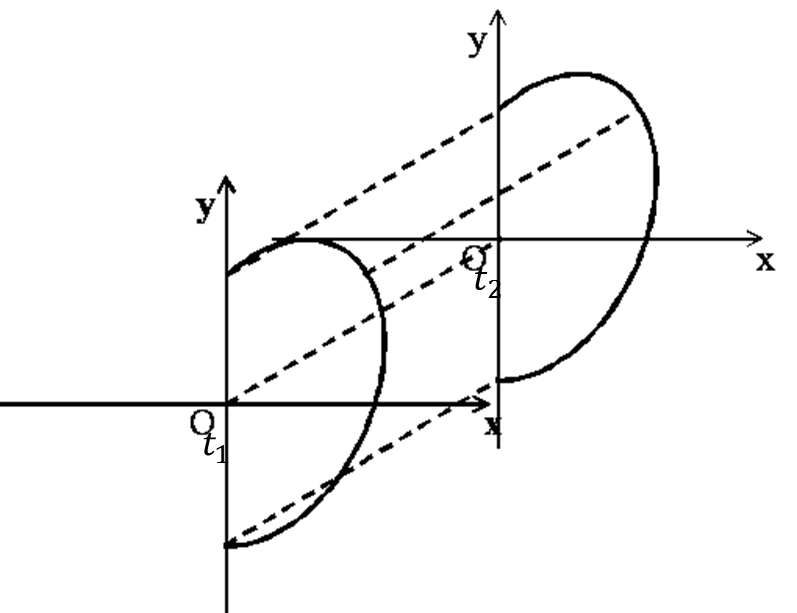
\includegraphics[height=4cm]{images/3.jpg}
            \caption{心形图的移动}
            \label{fig:心形图的移动}
            \end{figure}
            \noindent 图(\ref{fig:心形图的移动})表示图形从$t_1$时刻移动到$t_2$时刻,图中坐标点$O_{t_1}$移动到$O_{t_2}$ 。我们可以根据点平移规律“左加右减上加下减”来计算 $t_2$ 时刻到图中各点的坐标。
        \subsubsection{心形图的代码}
            \par
            心形图的绘图主程序为love.m,其调用了plot$\_$rose函数,plot$\_$rose用于绘制玫瑰花图,这个程序是在网络上找到的。此外,scaling函数用于对函数图像进行缩放。由于love程序过长,这里我们仅给出scaling函数
            \begin{lstlisting}[language = Matlab]
            function B = scaling(A, l)
            % A为原函数图上各点坐标
            % l为放缩长度
            % B为放缩后各点坐标
            B = zeros(size(A));
            n = length(A);
            L = zeros(n, 1);
            for i = 1:n
                if A(i,1)>0
                    L(i) = l;
                else
                    L(i) = -l;
                end
            end
            theta = atan(A(:,2)./A(:,1));
            B(:,1) = A(:,1)+L.*cos(theta);
            B(:,2) = A(:,2)+L.*sin(theta);
            \end{lstlisting}

        \subsubsection{心形图结果}
            \par
            下面,我们仅给出心形图的静态结果,如图(\ref{心形图运行结果})所示。心形图的动态结果可以自行运行程序 love.m查看。
                \begin{figure}[htbp]
                    \centering
                    \begin{subfigure}[b]{0.4\textwidth}
                        
\includegraphics[width=\textwidth]{images/44.png}
                        \caption{}
                        \label{爱心萌芽}
                    \end{subfigure}
                    \begin{subfigure}[b]{0.4\textwidth}
                        
\includegraphics[width=\textwidth]{images/45.png}
                        \caption{}
                        \label{因你而精彩}
                    \end{subfigure}
                    \begin{subfigure}[b]{0.4\textwidth}
                        
\includegraphics[width=\textwidth]{images/46.png}
                        \caption{}
                        \label{我的心满满的都是你}
                    \end{subfigure}
                    \begin{subfigure}[b]{0.4\textwidth}
                        
\includegraphics[width=\textwidth]{images/47.png}
                        \caption{}
                        \label{onlyforyou}
                    \end{subfigure}
                    \caption{心形图运行结果}
                    \label{心形图运行结果}
                \end{figure}

    \subsection{地形图}
        \subsubsection{地形图的目标}
            \par
            下面这个模型用到的工具箱(toolbox)包括:MATLAB自带的地图工具箱mapping toolbox和MMAP\footnote{https://www.eoas.ubc.ca/~rich/map.html}(A mapping package for MATLAB)。地形图模型的目标是:
            \begin{enumerate}
              \item 绘制地球仪,并highlight中国部分;
              \item 确定地球形状大小以及任意经纬度$(\varphi,\theta)$下的$(x,y,z)$坐标;
              \item 在某经纬度下插中国国旗
                \begin{enumerate}
                  \item 旗杆:给定杆长$l$后,计算地球表面$(\varphi,\theta)$点的法线方程并计算旗杆顶点的坐标。
                  \item 旗面:确定杆长以及杆两个端点的坐标后,确定旗面的$OZ$平面,并且允许旗面旋转一定角度。
                  \item 绘制五角星。
                \end{enumerate}
            \end{enumerate}
        \subsubsection{地形图建模(写程序前的研究过程)}
            \par
            \checkmark \textbf {我们可以利用geoshow绘制地球仪,这里不详细介绍。}
            \par
            \checkmark \textbf {根据地球大小形状建立空间直角坐标系并确定$(\varphi,\theta)$点的坐标$(x,y,z)$}
            \par
            地球的纵切面近似一个椭圆(MATLAB绘制的地球有些许差异,其实地球纵切面是一个类似鸡蛋的形状,这里我们简单处理)如下图(\ref{fig:地球纵切面简化图})所示
            \begin{figure}[H]
            \centering
            
\includegraphics[height=4cm]{images/4.png}
            \caption{地球纵切面简化图}
            \label{fig:地球纵切面简化图}
            \end{figure}
            \noindent 其中:$a$为赤道半径,$b$为极半径,$O$为地心。
            二维椭圆的定义为
            \begin{equation*}
            \centering
            \frac {x^2}{a^2}+\frac{y^2}{b^2}= 1
            \end{equation*}
            椭圆离心率的计算公式为:
            \begin{equation*}
            \centering
            e= \sqrt{\frac {a^2+b^2}{a^2}}
             \end{equation*}
            根据离心率的计算公式,给定$a,b$或$a,e$,我们可以唯一确定一个椭圆。
            \par
            \begin{definition}[《解析几何》椭球面]
            \par
            在直角坐标系下,$\frac {x^2}{a^2}+\frac{y^2}{b^2}+\frac{z^2}{c^2}= 1$所表示的曲面称为椭球面,该式亦称为椭球面的标准方程。如果用坐标系平面$x=0/y=0/z=0$来截椭球,所截得的曲面皆为椭圆。椭球面的参数方程为:
            \begin{equation*}
            \left\{\begin{lgathered}
            x=a \cos\theta \cos\varphi\\
            y=a \cos \theta \sin\varphi\\
            z=c \sin\theta
            \end{lgathered} \right.
            \end{equation*}
            其中:$\theta \in[-\frac \pi2]$,$\varphi\in[0,2\pi]$ 。其示意图如图(\ref{fig:椭球面示意图})所示
            \begin{figure}[H]
            \centering
            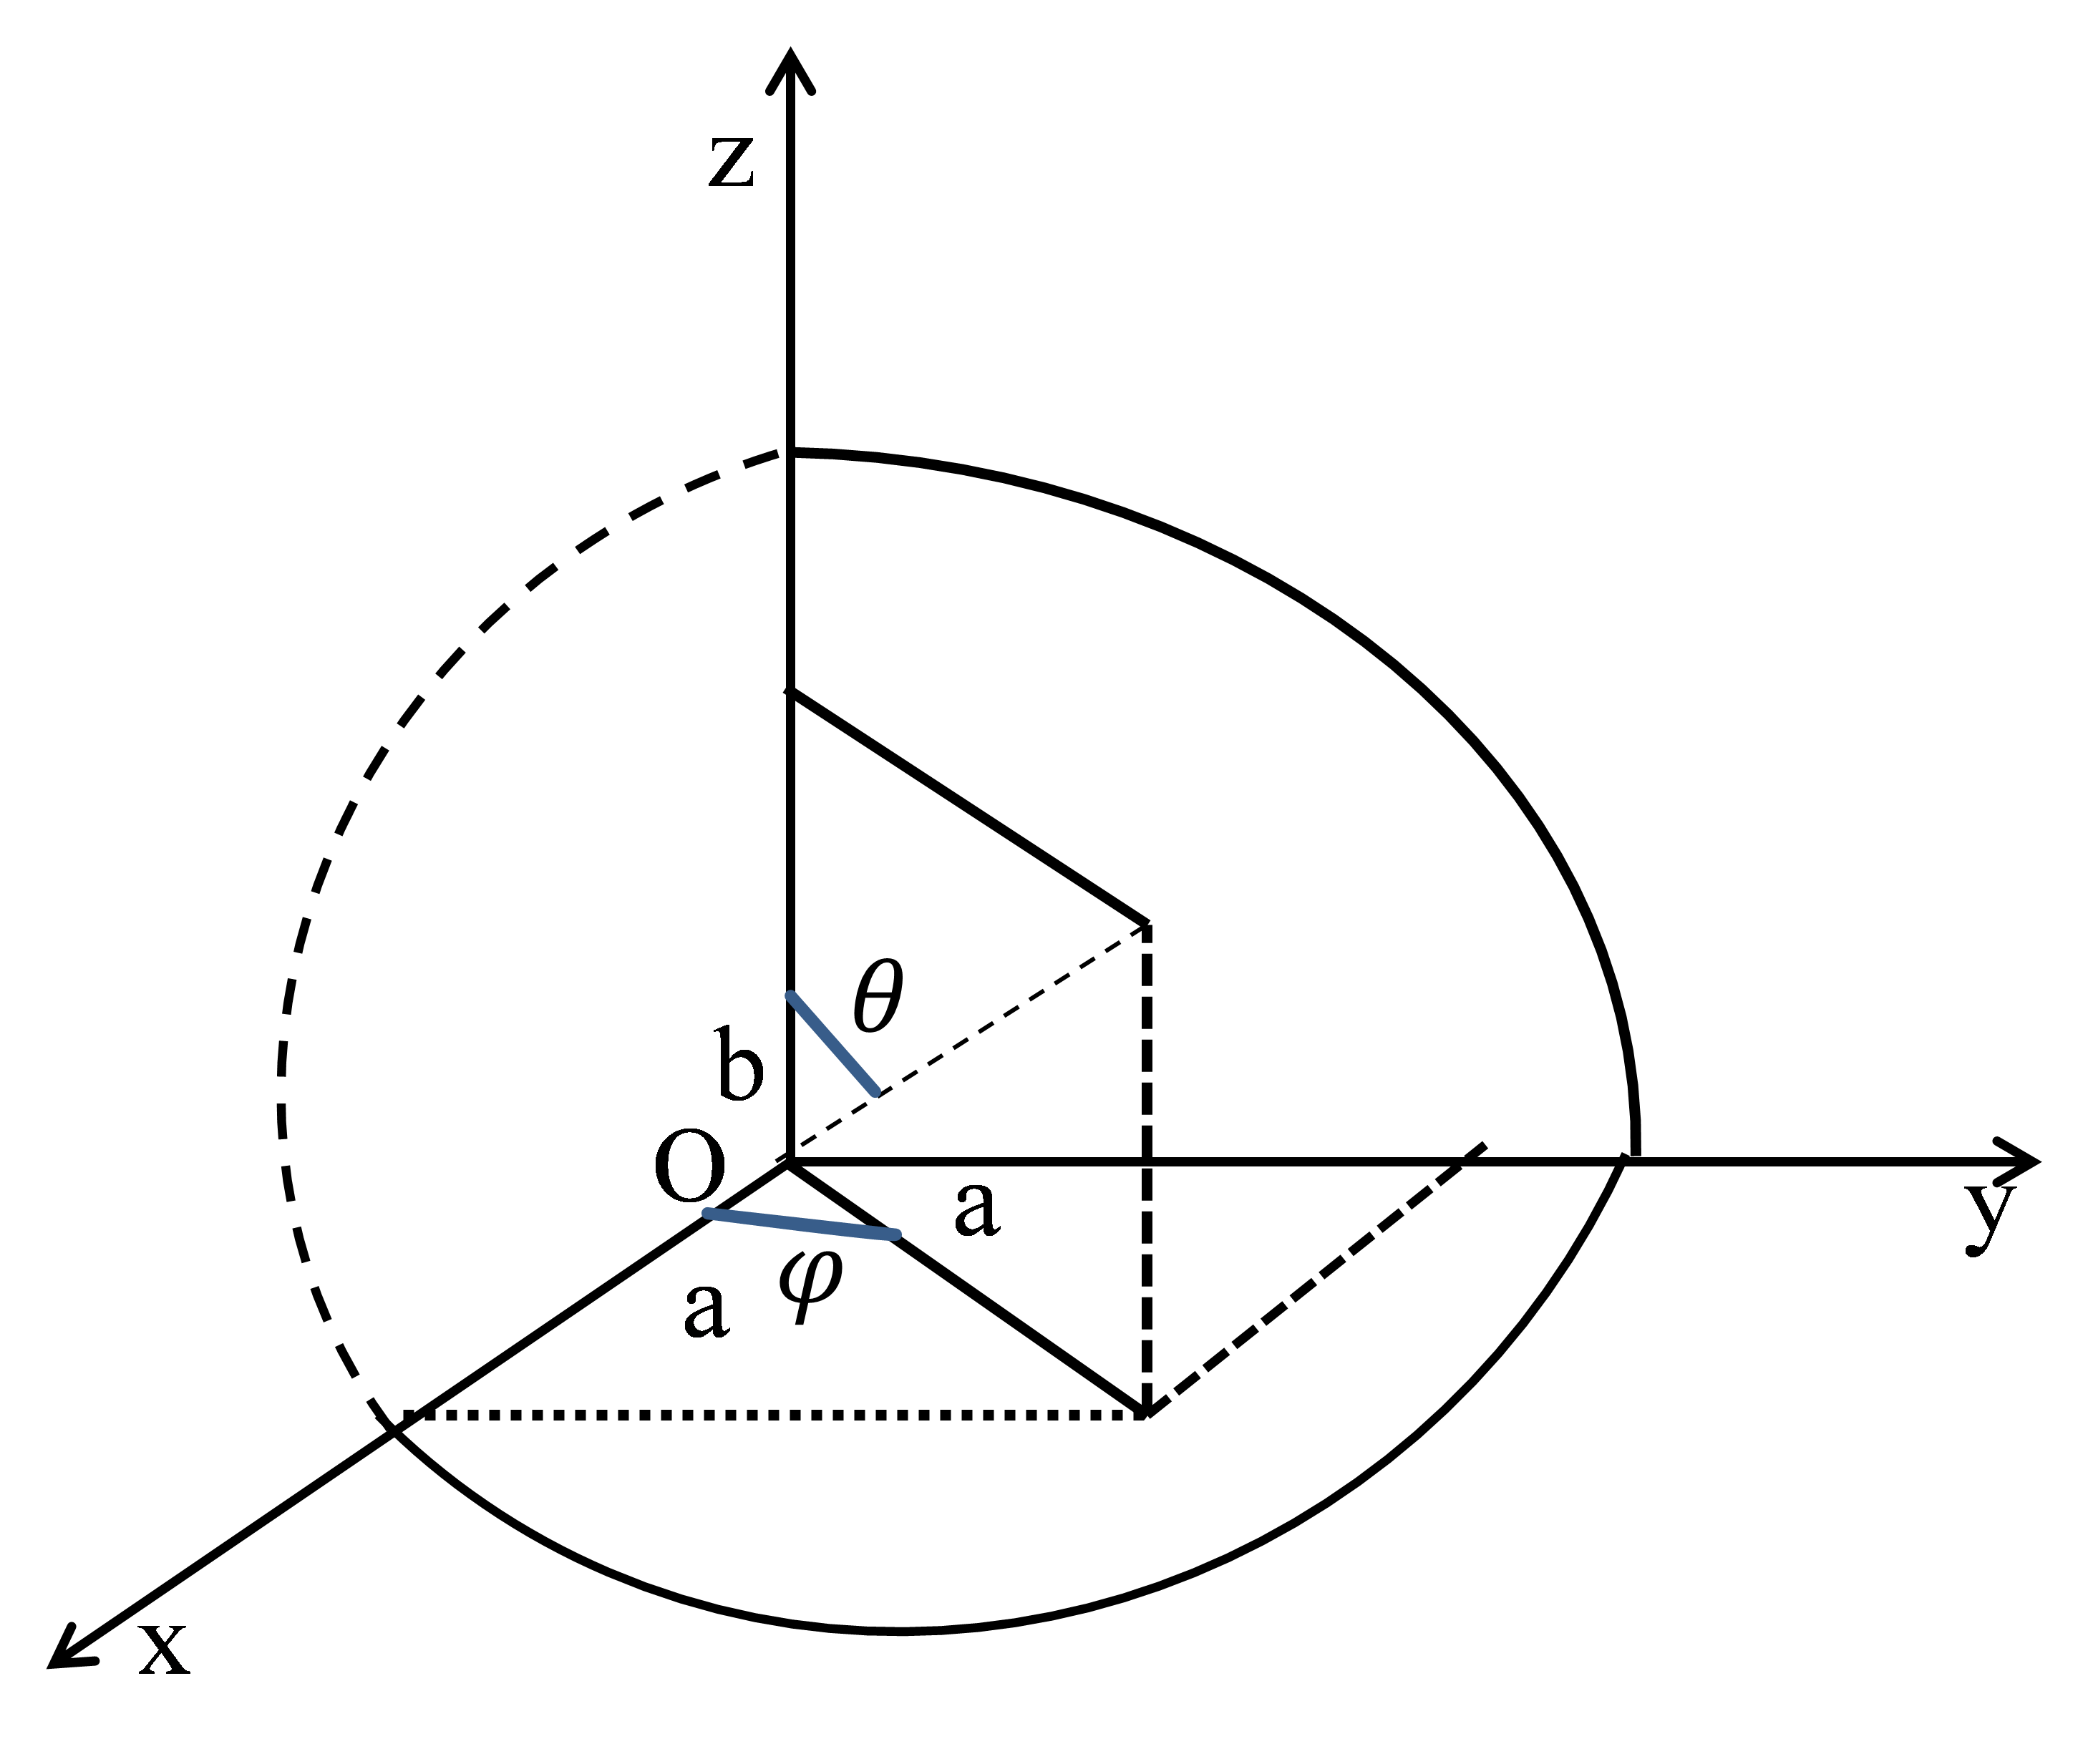
\includegraphics[height=4cm]{images/5.jpg}
            \caption{椭球面示意图}
            \label{fig:椭球面示意图}
            \end{figure}
            \end{definition}
            \par
            上面介绍的椭球面中的$(\varphi,\theta)$恰好对应经纬度。于是,对于给定的经纬度$(\varphi,\theta)$ ,有直角坐标:
            \begin{equation*}
             \left\{\begin{lgathered}
             x=a \cos\theta\cos\varphi\\
             y=a \cos \theta \sin\varphi\\
             z=c \sin\theta
             \end{lgathered} \right.
            \end{equation*}
            其中:$a = b=6378.1km,c=6356.8km,e=0.0579$ 。
            \par
            \checkmark \textbf {求 $(\varphi,\theta)$ / $(x,y,z)$点的法线方程,并计算旗杆顶点坐标}
            \par
            \textbf{引入:曲面的切平面与法线方程}
            \par
            设3维曲面为$S$,曲面$S$通常有下面3种表达方式
            \begin{align}
             & z =f(x,y)\\
             & F(x,y,z) =0\\
             & \left\{
             \begin{lgathered}
             x=x(u,v)\\
             y=y(u,v)\\
             z=z(u,v)
             \end{lgathered} \right.
            \end{align}
            这里我们选择第2种表示方式表示曲面,则S在$M_0=(x_0,y_0,z_0)$ 的切平面为
            \begin{equation*}
             \frac{\partial F}{\partial x}\Big|_{M_0} (x-x_0)+\frac{\partial F}{\partial y}\Big|_{M_0} (y-y_0)+\frac{\partial F}{\partial z}\Big|_{M_0} (z-z_0)=0
            \end{equation*}
            法线方程为
            \begin{equation*}
            \frac{x-x_0}{ \frac{\partial F}{\partial x}\big|_{M_0} }=\frac{y-y_0}{\frac{\partial F}{\partial y}\big|_{M_0} }=\frac{z-z_0}{\frac{\partial F}{\partial z}\big|_{M_0} }
            \end{equation*}
            于是,当我们给定杆长$l$以及杆与面$S$交点$M_0=(x_0,y_0,z_0)$后,可以求出旗杆顶点,其示意图如下图(\ref{旗杆顶点求解示意图})所示
            \begin{figure}[H]
            \centering
            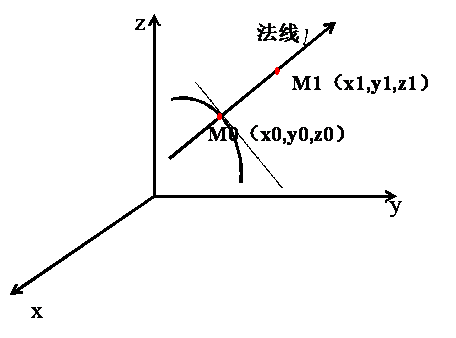
\includegraphics[height=4cm]{images/6.jpg}
            \caption{旗杆顶点求解示意图}
            \label{旗杆顶点求解示意图}
            \end{figure}
            可以通过下式求解杆顶点$M_1=(x_1,y_1,z_1)$的坐标
            \begin{equation*}
            \left\{\begin{lgathered}
            \frac{x_1-x_0}{ \frac{\partial F}{\partial x}\big|_{M_0} }=\frac{y_1-y_0}{\frac{\partial F}{\partial y}\big|_{M_0} }=\frac{z_1-z_0}{\frac{\partial F}{\partial z}\big|_{M_0} }\\
            (x_1-x_0)^2+(y_1-y_0)^2+(z_1-z_0)^2={\textit{l}}^2
            \end{lgathered} \right.
            \end{equation*}
            上述方程有两个可行解,为此我们添加约束条件($M_1$点在椭圆处):
            \begin{equation*}
            \centering
            s.t.\quad \frac{x_1^2}{ a^2}+\frac{y_1^2}{b^2}+\frac{z_1^2}{c^2}>1
             \end{equation*}
            其中,$a=b=6378.1km,c=6356.8km$。
            \par
            \checkmark \textbf {在旗杆上标记小红旗}
            \par
            上面,通过求偏导数以及解方程组,我们求得了旗杆端点的坐标$M_0=(x_0,y_0,z_0)$ 和$M_1=(x_1,y_1,z_1)$ 。接下来,我们的任务是绘制小红旗,未旋转前的红旗如图(\ref{fig:红旗未旋转前的示意图})所示
           \begin{figure}[H]
                \centering
                \begin{subfigure}[b]{0.25\textwidth}
                    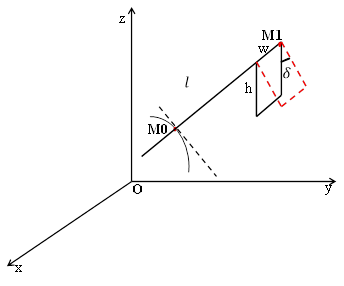
\includegraphics[width=\textwidth]{images/7.jpg}
                    \caption{}
                     \label{fig:红旗未旋转前的示意图小}
                \end{subfigure}
                \qquad
                \begin{subfigure}[b]{0.25\textwidth}
                    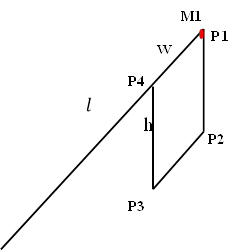
\includegraphics[width=\textwidth]{images/8.jpg}
                    \caption{}
                    \label{fig:红旗未旋转前的示意图大}
                \end{subfigure}
                \caption{红旗未旋转前的示意图}
                \label{fig:红旗未旋转前的示意图}
            \end{figure}
            设旗面未旋转前,$\overrightarrow{OZ}$在旗面上,旋转角度为 $\delta$,如图(\ref{fig:红旗未旋转前的示意图小})所示。图(\ref{fig:红旗未旋转前的示意图大})为红旗的放大图,其$P_1=M_1$,$w$为旗面的宽,$h$为旗面的长。我们先来求点$P_2$。$ P_{2}$在旗杆的垂线上,解下面方程组可求得$ P_{2}$的坐标\footnote{注:也可以用比例直接求解。}
            \begin{equation*}
            \left\{\begin{lgathered}
             \frac{\left |\overrightarrow{M_1P_2}\right |}{\left |\overrightarrow{M_1M_0}\right |}=\frac{\textit{w}}{\textit{l}}\\
             \frac{P_{2}x-x_{0}}{a}=\frac{P_{2}y-y_{0}}{b}=\frac{P_{2}z-z_{0}}{c}
             \end{lgathered} \right.
             \end{equation*}
            其中:$P_2x,P_2y,P_2z$为$P_2$点的坐标。上述方程组有两个解,我们在这里给出约束条件:
            \begin{equation*}
            \centering
            s.t.\left\{\begin{lgathered}
            x_1^2+y_1^2+z_1^2>P_{2}x^{2}+P_{2}y^{2}+P_{2}z^{2}\\
            M_{1}\text{在}P_{2}\text{外}
             \end{lgathered} \right.
             \end{equation*}
            \par
            下面来求点$ P_{3}$ ,点$ P_{3}$有3个特性:
            \begin{equation*}
            \centering
            \left\{\begin{lgathered}
            \overrightarrow{P_{2}P_{3}}\perp\overrightarrow{P_{2}P_{1}}\\
            \left|\overrightarrow{P_{2}P_{3}}\right|=h\\
            P_{3}\text{在旗面上}
             \end{lgathered} \right.
             \end{equation*}
            上述求解的关键点是$P_{3}$在旗面上,而旗面未知,所以我们先来求解旗面。未旋转之前,
            $\overrightarrow{OZ}$在旗面上,于是$z$轴上任意一点皆在旗面上。
            由此,我们得到了旗面的3个坐标点$M_1=(x_1,y_1,z_1)$,$P_2=(P_2x,P_2y,P_2z)$,$Z=(0,0,1)$  。
            \par
            \textbf{引入:平面的三点式方程}
            \par
            由空间中三个不共线的点构成的平面方程为:
            \begin{equation*}
            \centering
            \begin{vmatrix}
            x-x_{1}&y-y_{1}&z-z_{1}\\
            x_{2}-x_{1}&y_{2}-y_{1}&z_{2}-z_{1}\\
            x_{3}-x_{1}&y_{3}-y_{1}&z_{3}-z_{1}
             \end{vmatrix} =0
             \end{equation*}
            或表示成
            \begin{equation*}
            \centering
            \begin{vmatrix}
            x&y&z&1\\
            x_{1}&y_{1}&z_{1}&1\\
            x_{2}&y_{2}&z_{2}&1\\
            x_{3}&y_{3}&z_{3}&1
             \end{vmatrix} =0
             \end{equation*}
             \par
             将$M_1=(x_1,y_1,z_1)$ $P_2=(P_2x,P_2y,P_2z)$ $Z=(0,0,1)$ 代入可以求得平面方程。设旗面为$Ax+By+Cz=D$
            于是,求解$P_{3}$的方程组为
            \begin{equation*}
            \centering
            \left\{\begin{lgathered}
            \overrightarrow{P_{2}P_{3}}\cdot\overrightarrow{P_{2}P_{1}}=0\\
            \left|\overrightarrow{P_{2}P_{3}}\right|=h\\
            A\cdot P_{3}x+B\cdot P_{3}y+C\cdot P_{3}z=D
             \end{lgathered} \right.
             \end{equation*}
            上述方程组有两个解,同样在这里我们也给出约束条件:
            \begin{equation*}
            \centering
            s.t.\quad P_{3}z<P_{2}z
             \end{equation*}
             \par
             对于点$P_{4}$的求解,可以仿照点$P_{3}$的方法,相应的约束条件为$P_{4}z<P_{1}z$。
            其中:$P_{4}z$表示点$P_{4}$的$z$坐标。以上过程求解了未旋转的旗面坐标,下面,我们对旗面进行旋转,其示意图如图(\ref{fig:旗面的旋转})所示
            \begin{figure}[H]
            \centering
            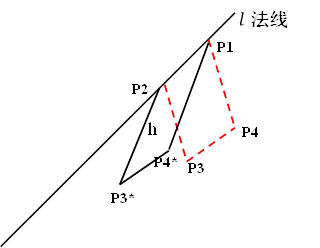
\includegraphics[height=3cm]{images/9.jpg}
            \caption{旗面的旋转}
            \label{fig:旗面的旋转}
            \end{figure}
            \noindent 其中:$\delta$ 为旋转角度,$P_{3}^{*}$、$P_{4}^{*}$为旋转后的旗面顶点。我们先来求 $P_{3}^{*}$:
            \begin{equation*}
            \centering
            \left\{\begin{lgathered}
            \overrightarrow{P_1P_3^*}\cdot \overrightarrow{P_2P_1}=0\\
            \left|\overrightarrow{P_1P_3^*}\right|=\omega
             \end{lgathered} \right.
             \end{equation*}
            上述方程有两个解,可以给出约束条件,也可以任意舍弃其中一个解。
            \par
            \checkmark \textbf{绘制五角星}
            \par
            至此,红旗的四个顶点 $P_{1}、P_{2}、P_{3}$和$P_{4}$已经确定。下面的工作是在旗面上绘制五角星,其示意图如下图(\ref{五角星示意图})所示
            \begin{figure}[H]
              \centering
              \begin{varwidth}[t]{\textwidth}
                \vspace{0pt}
                
\includegraphics[height=3cm]{images/10.jpg}
              \end{varwidth}
              \qquad \qquad
              \begin{varwidth}[t]{\textwidth}
                \vspace{0pt}
                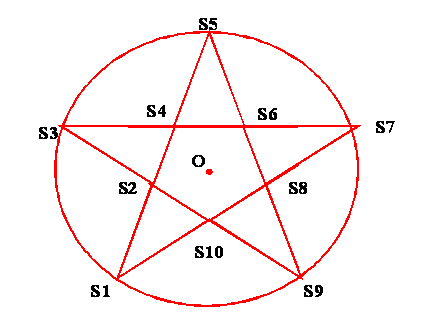
\includegraphics[height=3cm]{images/11.jpg}
              \end{varwidth}
              \caption{五角星示意图}
              \label{五角星示意图}
            \end{figure}
            \noindent 其中:$O$ 为五角星的外接圆心,$r$ 为外接圆的半径,$S_{1}$ 到$S_{10}$ 为五角星的顶点。下面我们来确定各五角星在红旗上的位置。\\
            \textbf{step1:根据《国旗制作法说明》确定五角星的位置}
            \begin{enumerate}
              \item 旗面为红色,形状为长方形且长与宽的比例为3:2;
              \item 大五角星的外接圆直径为旗高的十分之三;小星的外接圆直径为旗高十分之一。
              \item 五角星的位置与画法:
                \begin{enumerate}
                   \item 将旗面对分成四个相等的长方形,将靠杆上方长方形上下划分十等分,左右划分十五等分;
                    \item 大五角星中心在该长方形上五下五,左五右十处;
                    \item 小五角星的中心: 第1个在上二下八,左十右五处;第2个在上四下六,左十二右三处;第3个在上七下三,左十二右三处;第4个在上九下一,左十右五处;
                    \item 四个小五角星各自必有一外顶点(奇数顶点)位于大五角星与自身小五角星中心的连线上;
                \end{enumerate}
            \end{enumerate}
            \textbf{step2:将旗面对折,形成4个相等矩形,其示意图如图(\ref{fig:旗面对折示意图})所示}
            \begin{figure}[H]
            \centering
            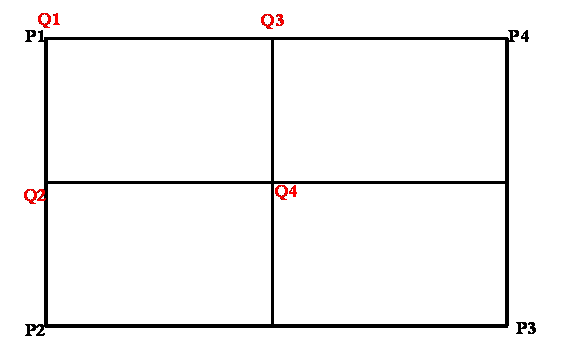
\includegraphics[height=4cm]{images/12.jpg}
            \caption{ 旗面对折示意图 }
            \label{fig:旗面对折示意图}
            \end{figure}
            其中:
            \begin{equation*}
            \centering
            \left\{\begin{lgathered}
            Q_{2}=\frac{P_{1}+P_{2}}{2}=0\\
            Q_{4}=\frac{P_{1}+P_{4}}{2}=0\\
            \end{lgathered} \right.
            \end{equation*}
            这里我们并不需要求解$Q_{3}$ 。
            然后,将得到的四分之一旗面($Q_{1}$,$Q_{2}$ ,$Q_{3}$ ,$Q_{4}$)的$Q_{1}Q_{2}$边十等分,$Q_{1}Q_{4}$边15等分(可以使用linspace ($Q_{1x}$,$Q_{2x}$ ,10),\textit{linspace}($Q_{1y}$,$Q_{2y}$ ,10),\textit{linspace}($Q_{1z}$,$Q_{2z}$ ,10))。至此,10乘15的刻度及各点坐标可以得到,记为tick。\\
            \textbf{Step3:确定大圆圆心及直径$d_{\text{大}}$}
            \begin{equation*}
            \centering
            \left\{\begin{lgathered}
            d_{\text{大}}=\frac{3}{10}w\\
            r_{\text{大}}=\frac{1}{2}d_{\text{大}}\\
             \end{lgathered} \right.
             \end{equation*}
            其中:$w$为旗面的宽。下面,求解大圆圆心坐标$O_{\text{大}}(x,y,z)$,其示意图如图(\ref{fig:旗面大圆圆心坐标示意图})所示
            \begin{figure}[H]
            \centering
            
\includegraphics[height=4cm]{images/13.jpg}
            \caption{旗面大圆圆心坐标示意图}
            \label{fig:旗面大圆圆心坐标示意图}
            \end{figure}
            \noindent 其中:A为上五下五点,B为左五右十点,在tick里均有说明。$O_{\text{大}}$的求解方程组如下
            \begin{equation*}
            \centering
            \left\{\begin{lgathered}
            \overrightarrow{AO_{\text{大}}}\cdot\overrightarrow{AO_{\text{大}}}=0\\
            \overrightarrow{AO_{\text{大}}}\cdot\overrightarrow{Q_1Q_2}=0\\
            \left|\overrightarrow{AO_{\text{大}}}\right|=\frac{1}{2}\left|\overrightarrow{Q_1Q_2}\right|
            \end{lgathered} \right.
            \end{equation*}
            \par
            这个问题可以表述为:空间中,给定长方形三个顶点,如何求解第四个顶点。\\
            \textbf{step4:确定小圆圆心$Q_{1}$,$Q_{2}$ ,$Q_{3}$ ,$Q_{4}$及圆的直径$d_{\text{小}}$。}小圆圆心求法如同大圆
            \begin{equation*}
            \centering
            \left\{\begin{lgathered}
            d_{\text{小}}=\frac{1}{10}w\\
            r_{\text{小}}=\frac{1}{2}d_{\text{小}}=\frac{1}{20}w\\
             \end{lgathered} \right.
             \end{equation*}
            \textbf{Step5:画五角星以及五角星的转向}
            \par
            下面,我们来研究如何绘制空间五角星,其示意图如图(\ref{空间五角星示意图})所示
            \begin{figure}[H]
            \centering
            \begin{subfigure}[b]{0.4\textwidth}
                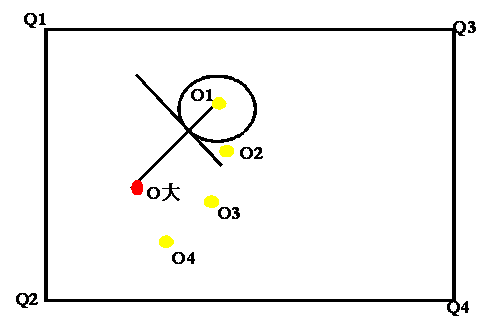
\includegraphics[width=\textwidth]{images/14.jpg}
                \caption{}
            \end{subfigure}
            \begin{subfigure}[b]{0.4\textwidth}
                
\includegraphics[width=\textwidth]{images/15.jpg}
                \caption{}
            \end{subfigure}
            \caption{空间五角星示意图}
            \label{空间五角星示意图}
            \end{figure}
            其中,$O$为圆心,$S_{1}$到$S_{10}$为五角星的顶点。我们可以利用结构体数组来存放五角星的信息,并且考虑到绘制五角星时要求五角星有一外顶点要在大小圆心的连线上,我们先假设可以求得该外顶点(例如$S_{1}$)。于是问题就转化为:在已有$S_{1}$的情况下如何确定其余顶点坐标。
            \par
            对于一个五角星,我们已知其圆心$O$,顶点$S_{1}$及半径$r$,有很多方法可以求解$S_{2}$,$S_{3}$。
            \par
            \ding{172}方法1:先看点$S_{3}$:$S_{3}$点在旗面上、与$O$点距离为$r$且$\angle{S_{1}OS_{3}}=72^\circ$,由此可以列出$S_{3}$的求解方程组为
            \begin{equation*}
            \centering
            \left\{\begin{lgathered}
            AS_3x+BS_3y+CS_3z=D\\
            (S_3x-O_x)^2+(S_3y-O_y)^2+(S_3z-O_z)^2=r\\
            \cos(\overrightarrow{OS_1},\overrightarrow{OS_3})=\frac{\overrightarrow{OS_1}\cdot\overrightarrow{OS_3}}{\left|\overrightarrow{OS_1}\right|\cdot\left|\overrightarrow{OS_3}\right|}=\cos(72^\circ)
             \end{lgathered} \right.
            \end{equation*}
            解此方程组,有两个可行解,除$S_{3}$外,另一个可行解为$S_{4}$,所以两者皆保留。
            \par
            再看$S_{2}$点。$S_{2}$点的求解方法和$S_{3}$点是一样的,不过我们不知道$\overrightarrow{OS_2}$的模以及$\angle{S_{1}OS_{2}}$的角度,为此我们先来求解二者,五角星示意图如图(\ref{fig:五角星示意图})所示
            \begin{figure}[H]
            \centering
            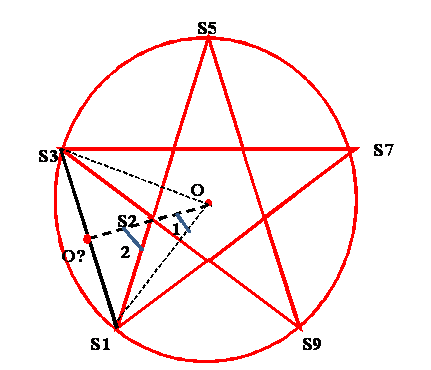
\includegraphics[height=4cm]{images/16.jpg}
            \caption{五角星示意图}
            \label{fig:五角星示意图}
            \end{figure}
            问题描述为:已知 $OS_3$, $OS_1$长为$r$,$\angle{S_{1}OS_{3}}=72^\circ$,求$OS_2$长及$\angle{S_{1}OS_{2}}$。求解该问题:
            \begin{equation*}
            \centering
            \left\{\begin{lgathered}
            \angle{S_1OS_3}=72^\circ\\
            \angle{S_1OS_2}=\frac{1}{2}\angle{S_1OS_3}=36^\circ\\
            \angle{S_1S_2S_3}=2(\angle{OS_1S_5}+\angle{S_1OS_2})=2(18^\circ+36^\circ)=108^\circ\\
            OS_2=OO'-O'S_2=r\cdot \cos\angle{1}-r\cdot \frac{\sin\angle{1}}{\tan\angle{2}}
            \end{lgathered} \right.
             \end{equation*}
            因此,我们可以计算出顶点$S_2$的坐标
            \begin{equation*}
            \centering
            \left\{\begin{lgathered}
            AS_2x+BS_2y+CS_2z=D\\
            (S_2x-O_x)^2+(S_2y-O_y)^2+(S_2z-O_z)^2=OS_2^2\\
            \cos(\overrightarrow{OS_1},\overrightarrow{OS_2})=\frac{\overrightarrow{OS_1}\cdot\overrightarrow{OS_2}}{\left|\overrightarrow{OS_1}\right|\cdot\left|\overrightarrow{OS_2}\right|}=\cos(36^\circ)
             \end{lgathered} \right.
            \end{equation*}
            解上述方程,同样会有两个解,一个是$S_2$一个是$S_1$ 。
            \par
            \ding{173}方法2:对于偶数顶点$S_2$,可以在求出奇数顶点后用直线相交的方法求解$S_2$($S_2$是线$S_1S_5$和线$S_3S_9$ 的交点),这里不做详细叙述。
            \par
            前面我们假设已知$S_1$,下面我们将其求解出来。大五角星的点$S_1$的确定如图(\ref{fig:大五角星角的确定})左所示。
            \begin{figure}[H]
              \centering
              \begin{varwidth}[t]{\textwidth}
                \vspace{0pt}
                
\includegraphics[height=3cm]{images/17.jpg}
              \end{varwidth}
              \qquad
              \begin{varwidth}[t]{\textwidth}
                \vspace{0pt}
                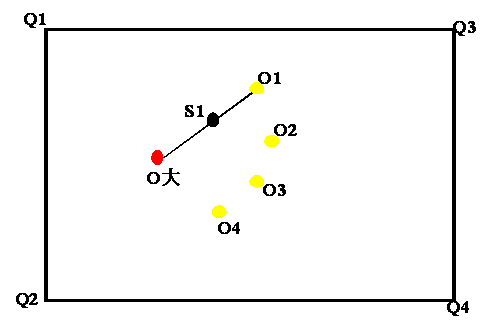
\includegraphics[height=3cm]{images/18.jpg}
              \end{varwidth}
            \caption{大五角星角的确定}
            \label{fig:大五角星角的确定}
            \end{figure}
            \noindent 由上图得,$\left|\overrightarrow{O_{\text{大}}S_1}\right|=r$, $\left|\overrightarrow{O_{\text{大}}B}\right|=\frac{1}{2}\left|\overrightarrow{Q_1Q_2}\right|$,且$S_1$在旗面上,于是有下面的方程:
            \begin{equation*}
            \centering
            \left\{\begin{lgathered}
            AS_1x+BS_1y+CS_1z=D\\
            \overrightarrow{AO_{\text{大}}}\cdot\overrightarrow{Q_1Q_2}=0\\
            \frac{\left|\overrightarrow{O_{\text{大}}S_1}\right|}{\left|\overrightarrow{O_{\text{大}}B}\right|}=\frac{r}{\frac{1}{2}\left|\overrightarrow{Q_1Q_2}\right|}=\frac{r}{\frac{1}{4}w}
             \end{lgathered} \right.
             \end{equation*}
            求上述方程,会有两个解,因此给出约束条件:
            \begin{equation*}
            \centering
            s.t.\quad \left|\overrightarrow{S_1O_1}\right|<\left|\overrightarrow{S_1O_2}\right|
             \end{equation*}
             \par
            小五角星的点$S_1$的确定如图(\ref{fig:大五角星角的确定})所示,从中可以看到$S_1$在$O_1 O_{\text{大}}$直线上,且距离$O_1$为$r_{\text{小}}$。
            \begin{lemma}[直线的两点式方程]
            空间中用两点式确定的直线方程为
            \begin{equation*}
            \centering
            \frac{x-x_{1}}{x_{2}-x_{1}}=\frac{y-y_{1}}{y_{2}-y_{1}}=\frac{z-z_{1}}{z_{2}-z_{1}}
             \end{equation*}
            \end{lemma}
            \par
            由上述引理,可以得到求解$S_1$的方程组为
            \begin{equation*}
            \centering
            \left\{\begin{lgathered}
            \frac{S_1x-O_{\text{大}}x}{O_1x-O_{\text{大}}x}=\frac{S_1y-O_{\text{大}}y}{O_1y-O_{\text{大}}y}=\frac{S_1z-O_{\text{大}}z}{O_1z-O_{\text{大}}z}\\
            (S_1x-O_1x)^2+(S_1y-O_1y)^2+(S_1z-O_1z)^2=r_{\text{小}}^2
             \end{lgathered} \right.
            \end{equation*}
            解方程组会有两个解,对其进行约束,
            \begin{equation*}
            \centering
            s.t.\quad \left|\overrightarrow{O_{\text{大}}S_1}\right|<\left|\overrightarrow{O_{\text{大}}O_1}\right|
            \end{equation*}
            \par
            到这里,模型的的主干部分已经结束,而对于图形而言,还有很多琐碎的细节等待我们去处理。
\section{MATLAB的基本绘图命令}
    \subsection{MATLAB图形GUI界面介绍}
        \par
        对于绘制后的图形,我们可以通过鼠标点击的方式来修饰图形。我们用一个例子进入图形的GUI界面,然后介绍图形中的对象及其属性。例子使用plot绘图命令绘制$sin(x)$的$x$在$[0,2\pi]$的图形,运行下面的程序
        \begin{lstlisting}[language = Matlab]
        plot(linspace(0,2*pi,360),sin(linspace(0,2*pi,360))
        \end{lstlisting}
        得到如图(\ref{sin函数图像1})所示的图形
        \begin{figure}[H]
        \centering
        \begin{subfigure}[b]{0.4\textwidth}
            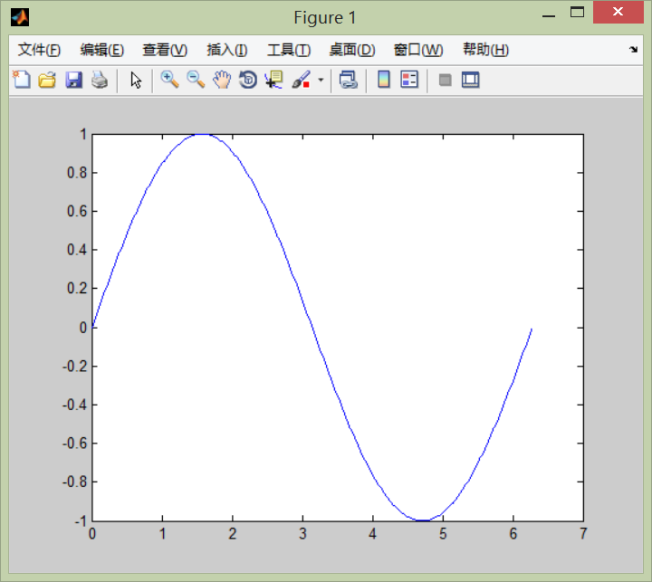
\includegraphics[width=\textwidth]{images/19.jpg}
            \caption{}
            \label{sin函数图像1}
        \end{subfigure}
        \begin{subfigure}[b]{0.4\textwidth}
            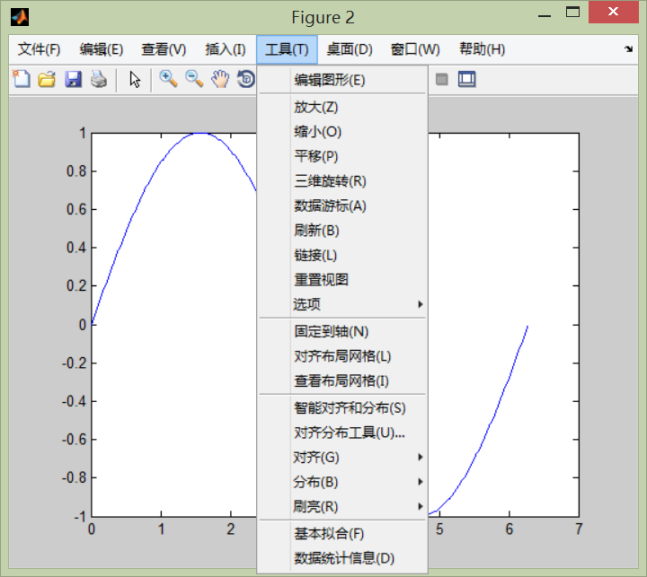
\includegraphics[width=\textwidth]{images/20.jpg}
            \caption{}
            \label{sin函数图像2}
        \end{subfigure}
        \caption{sin函数图像}
        \end{figure}
        \par
        这里我们给出的是图形窗口,如果需要保存图形,请自行查询方法。下面我们将详细分析这个图形窗口(关于绘图的相关命令,我们将其放在后面)。通过分析这个图形窗口,我们将学到:MATLAB图形中的对象有哪些,对象属性又有哪些。不要认为这是一个简单的窗口,首先,我们要观察窗口的菜单栏和工具栏(这两个名词真的很形象)
        菜单栏(第一栏)中有:文件、编辑、查看、插入、工具、调试桌面、窗口、帮助的菜单章节,就像餐厅里的菜单中有:主食、茶饮、酒等几个主要部分。
        点击进入菜单章节(例“工具”),你会看到详细的“菜肴”,如图(\ref{sin函数图像2})所示。这些“菜肴”的具体部分也可以在工具栏(第二栏)中找到,这里我们仅仅介绍两个工具(“菜肴”):基本拟合、数据统计分析。这两道“菜肴”真的为M图形工具增色不少。其“基本拟合工具”和EXCEL中的拟合功能相近;“数据统计分析”是描述统计分析。这两道“菜肴”的窗口命令如图(\ref{图形中的基本拟合和数据统计分析工具})所示(必须强调真的很好用,也特别容易上手)。
        \begin{figure}[H]
        \centering
        \begin{subfigure}[b]{0.2\textwidth}
            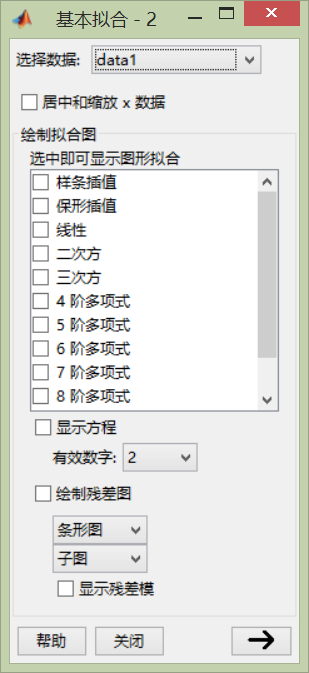
\includegraphics[width=\textwidth]{images/21.jpg}
            \caption{}
            \label{基本拟合}
        \end{subfigure}
        \begin{subfigure}[b]{0.4\textwidth}
            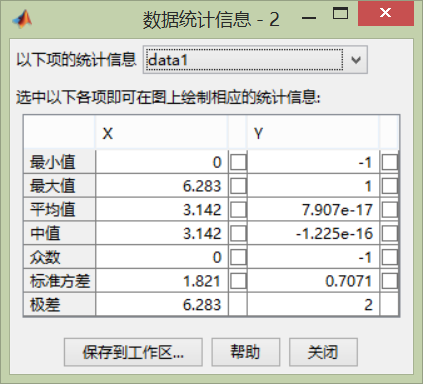
\includegraphics[width=\textwidth]{images/22.jpg}
            \caption{}
            \label{数据统计分析}
        \end{subfigure}
        \caption{图形中的基本拟合和数据统计分析工具}
        \label{图形中的基本拟合和数据统计分析工具}
        \end{figure}
        下面我们来看工具栏,需要指出的是,工具栏不仅只有窗口中显示的那几个工具。在菜单栏中点击“查看”,将下面的“菜肴”全部选上(只有前3个是工具栏,后面3个是重启),得到的窗口如图(\ref{图形窗口})所示,窗口的2,3,4栏是工具栏,你可以自行尝试这些工具的功能(你只需将鼠标放在相应的位置,就会有相应的说明)。对于图形选项板与绘图浏览器,在这里就不详细说明了,你可以点击下拉快捷按钮来查看该模块(选项板)下可以进行的操作,可以将其关闭或取消停靠。
        \begin{figure}[H]
        \centering
        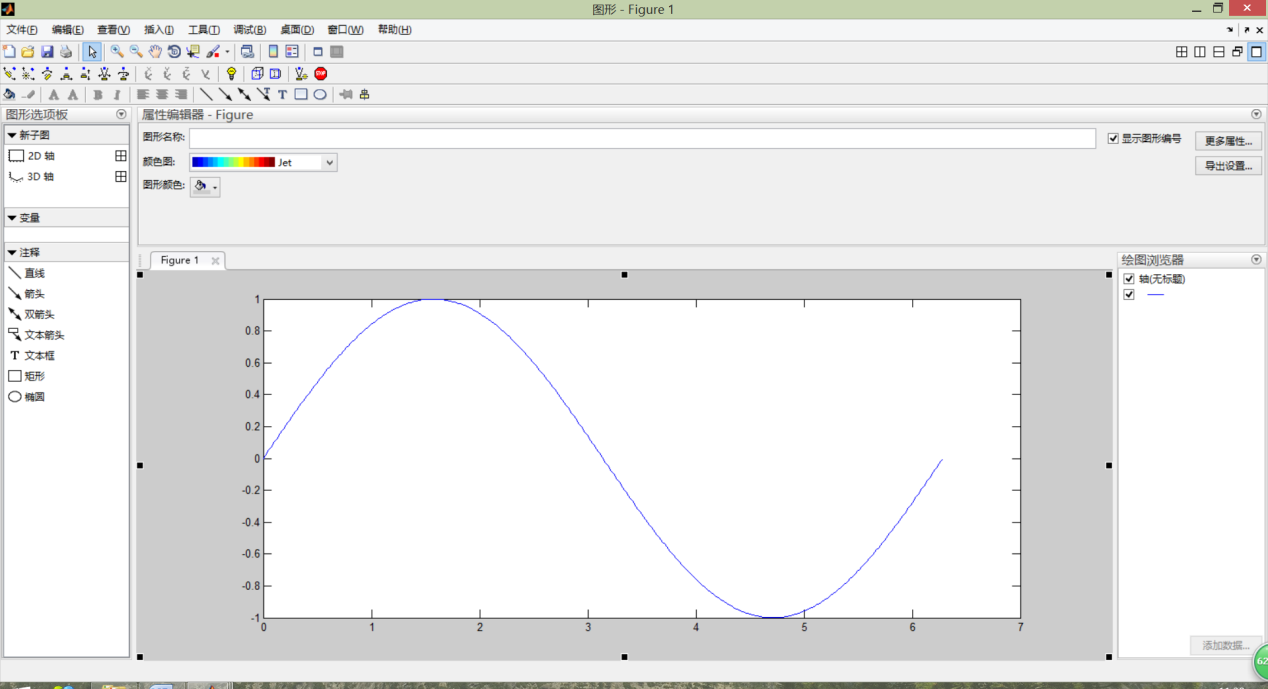
\includegraphics[height=8cm]{images/23.jpg}
        \caption{图形窗口}
        \label{图形窗口}
        \end{figure}
        下面,我们将详细介绍属性编辑器。先来看一下我们绘制的图形中都有哪些对象,然后查看每个对象对应的属性(属性编辑器)。图(\ref{图形中的对象})展示了我们的对象,其类似于绘画工具:画板、画布和画
        \begin{figure}[H]
        \centering
        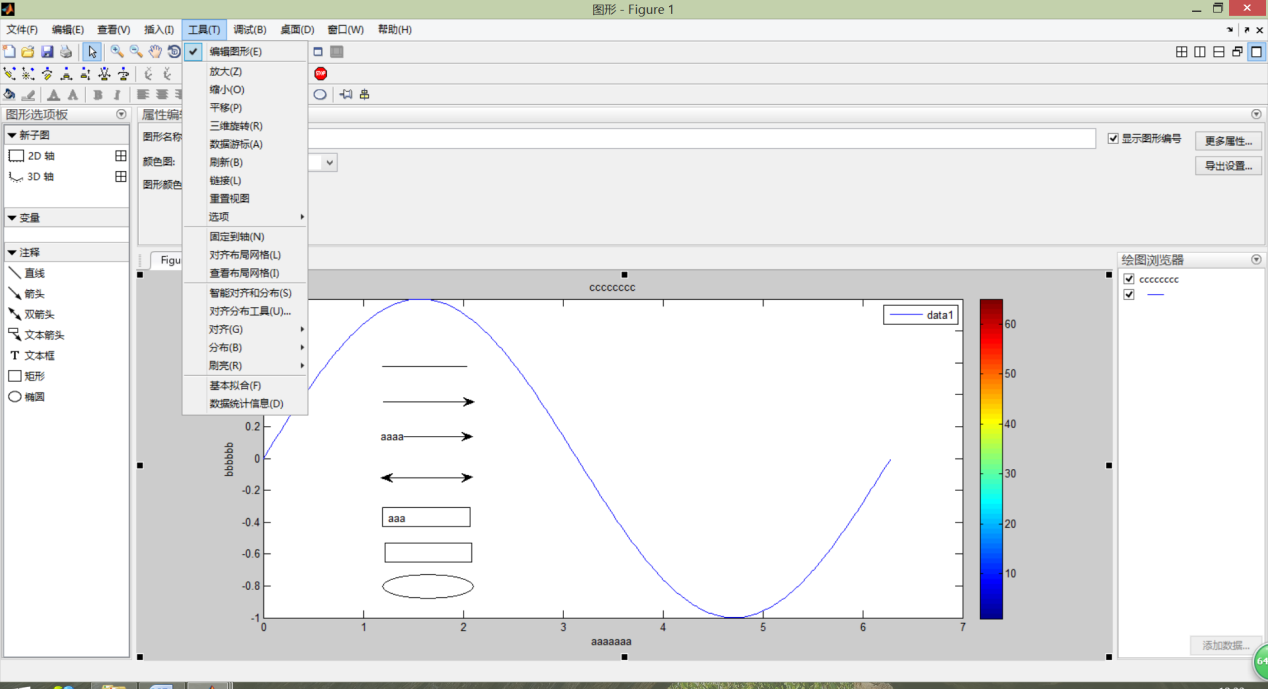
\includegraphics[height=8cm]{images/24.jpg}
        \caption{图形中的对象}
        \label{图形中的对象}
        \end{figure}
        \par
        可能存在的对象绝不仅有这些,我们可以在菜单栏下的“插入”中插入相应的对象:X标签、Y标签和标题(这3者是每张图必有的,其大部分为文本);图例、颜色栏colorbar;线、箭头$\dots$椭圆是用于注释的。我们将可插入的对象插入进来,如图(\ref{图形中的对象})所示。现在对象已经有了,接下来我们研究对象的属性(例:就像“线”对象,有线的粗细、长短、色等等)。
        \par
        对象有:figure、axes、line series、x lable/y lable/title(这三者是text文本对象)、textbox、scribe、scribe rect/ellipse、line/Arrow/double Arrow、legend。我们如何用命令获取对象属性?get set 用鼠标点击(选中)要研究的对象(例如figure),相应的属性编辑器会给出该对象的常用属性。我们选取右边的“更多属性”,进入“检查器:figure”,默认的属性排序是按照A→Z字母进行排序的。可以点击左上角的按键,进入属性的列表排序,如图(\ref{fig:figure的检查器}) 所示,我们给出了部分属性的中文名称以便于理解与查找。
        可以自行查看axes(轴)、lineseries(线序列)、xlable(text文本)、textbox(文本框)、scribe tect/ellipse(矩形椭圆)、scribe line/Arrow等(注释)的属性检查器
        \begin{figure}[H]
        \centering
        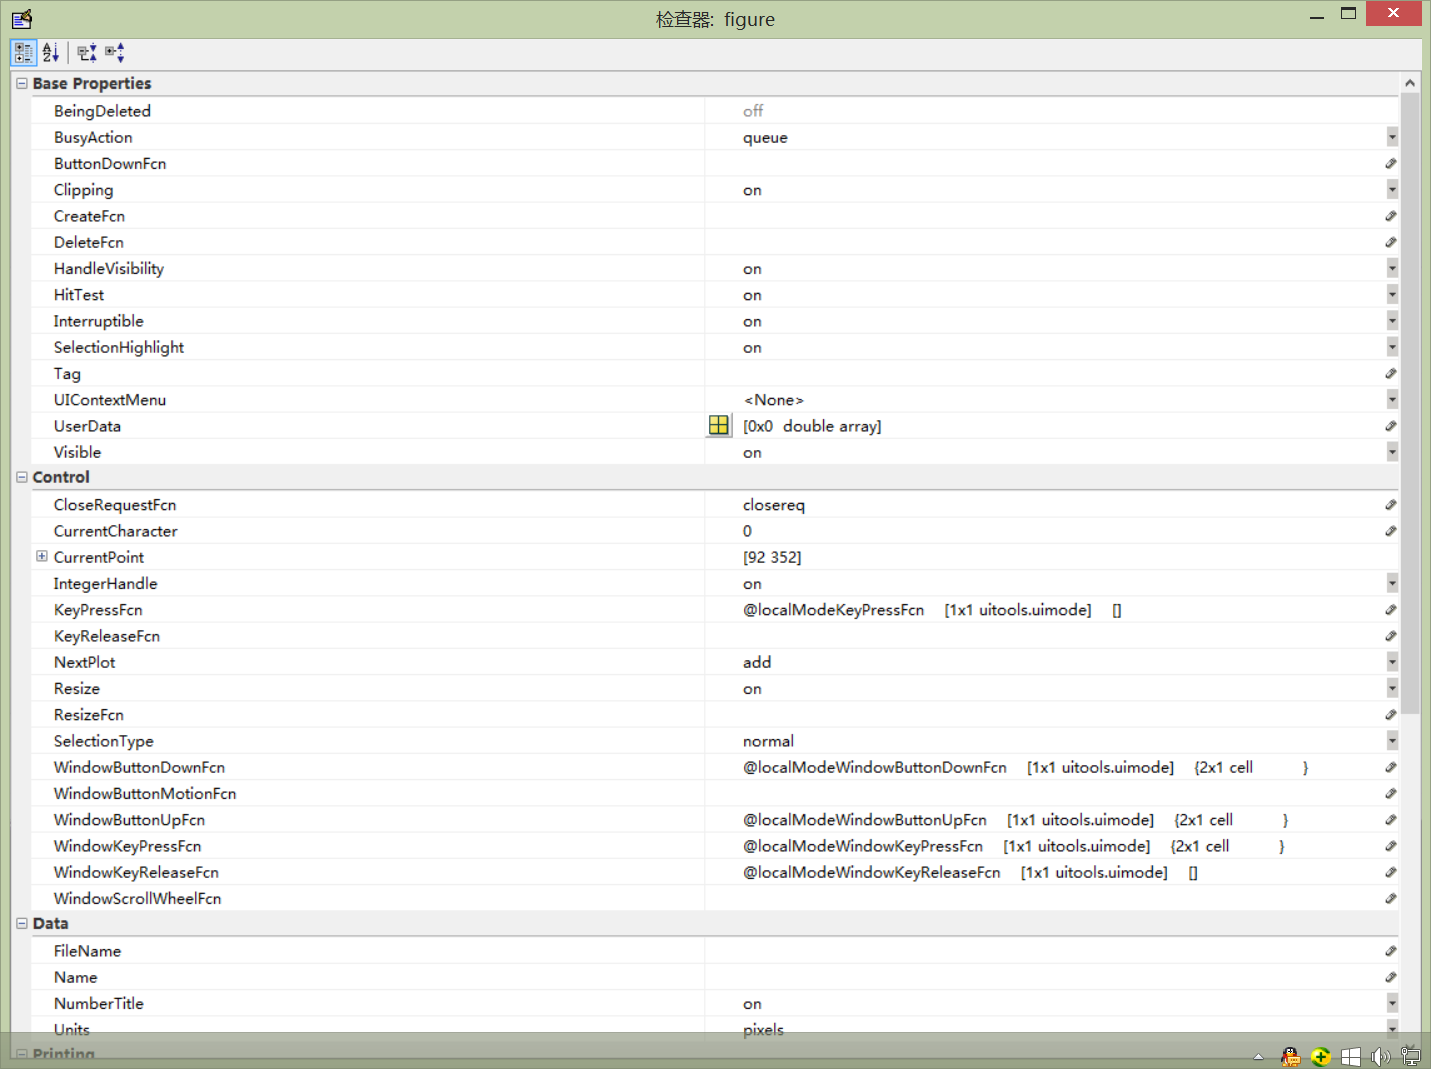
\includegraphics[width = 14cm]{images/25.jpg}
        \caption{figure的检查器}
        \label{fig:figure的检查器}
        \end{figure}
        \textbf{1.figure的属性如下}
        \begin{enumerate}
          \item Figure(图形)
            \begin{enumerate}
               \item base property\quad 基础性能
                \item control\quad 控制
                \item data\quad 数据
                  \begin{enumerate}
                   \item filename\qquad 文件名
                   \item name\qquad 图形名
                   \item Number Title\qquad on/off
                   \item Units单元:inches(英寸)centimeters(厘米)normalization(标准化)points(点)pixels(像素点)characters(特性)
                   \end{enumerate}
               \item printing\quad 打印
               \begin{enumerate}
                   \item  Invert handcopy  on/off
                   \item Paper orientation(纸方向)portrait(描写)landspace(风景)rotated(旋转)paper
                   \item position.X/Y/width/height
                   \item Paper position mode
                   \item Paper size.X/Y
                   \item Paper type
                   \item Paper units
                   \end{enumerate}
                \item style/Appearance\quad 风格/外观
                  \begin{enumerate}
                   \item  Color
                   \item RGB
                   \item DockControls  on/off
                   \item MenuBar(菜单)\qquad figure
                   \item Pointer(指针) \qquad arrow/crosshair(箭头/十字)
                   \end{enumerate}
            \end{enumerate}
        \end{enumerate}

        % \textbf{2.axes的属性如下}
        % \begin{enumerate}
        %   \item axes rules\qquad 标尺
        %   \begin{enumerate}
        %        \item xaxes location(位置)\qquad top/bottom
        %       \item xcolor(颜色)\qquad RGB
        %       \item xDir(方向)\qquad normal/reverse
        %       \item xgrid(网格)\qquad on/off
        %       \item xlim(限度)\qquad [x y]
        %       \item xlimMode\qquad normal/auto
        %       \item xMinorgrid(小标度网格)\qquad on/off
        %       \item xMinortick(小标度标记) \qquad on/off
        %       \item xscale
        %       \item xtick
        %       \item xticklable
        %       \item xticklablemode
        %     \end{enumerate}
        %   \item basic properties\qquad 基础性能
        %   \item camera\qquad 照相机
        %   \item color \qquad 颜色
        %         \begin{enumerate}
        %         \item Ambientlightcolor(环境颜色)
        %         \item Clim
        %         \item  Climmode
        %         \item Color(画布颜色)
        %         \item Colororder
        %           \end{enumerate}
        % \item control \qquad 控制
        % \begin{enumerate}
        %         \item currentpoint.X/Y
        %         \item DrawMode(画)\qquad normal/fast
        %         \item  NextPoint\qquad normal/fast
        %           \end{enumerate}
        % \item font\qquad 字体
        %          \begin{enumerate}
        %            \item  fontangle\qquad 角度\qquad normal/italinc(斜体)/
        %            \item fontname
        %            \item  fontunits
        %         \end{enumerate}
        %  \item position\qquad 位置
        %    \begin{enumerate}
        %         \item Active Position Property
        %         \item outer position(4)
        %         \item  position(4)
        %         \item  units
        %    \end{enumerate}
        %     \item style/appearance \qquad 基本外观
        %     \begin{enumerate}
        %          \item  Alim
        %          \item Alim mode
        %          \item Box\qquad on/off
        %          \item Data Aspect Ratio
        %          \item  Data Aspect Ratio Mode
        %          \item Grid linestyle
        %          \item Layer      bottom/top
        %          \item lineStyleMode
        %          \item lineWidth
        %          \item Minor Grid linestyle
        %          \item Plot Box Aspect Ratio
        %          \item Plot Box Aspect Ratio Mode
        %    \end{enumerate}
        %  \item tick \qquad 标记号
        %     \begin{enumerate}
        %         \item tick Dir(括号方向)
        %         \item tick Dir Mode
        %         \item tick length
        %         \item tight inset
        %     \end{enumerate}
        % \end{enumerate}
        % \begin{figure}[H]
        % \centering
        % 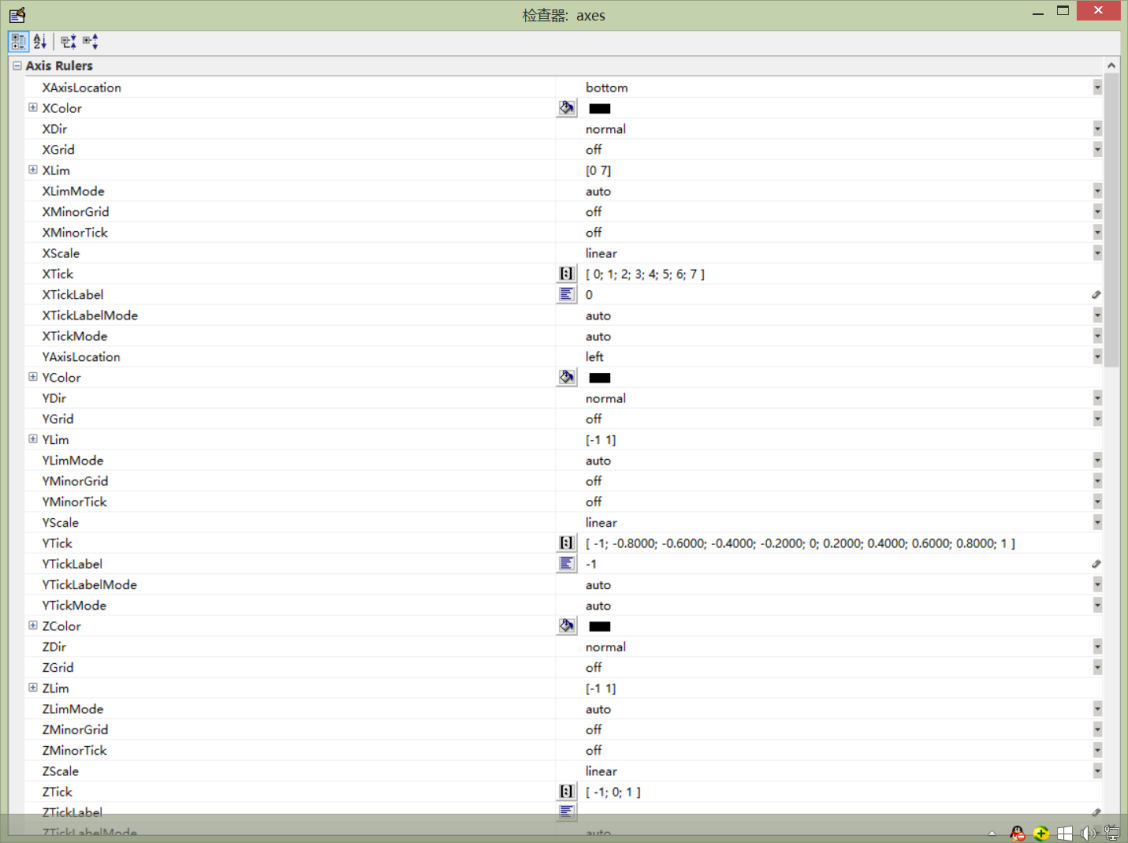
\includegraphics[height=4cm]{images/26.jpg}
        % \end{figure}
        % \begin{figure}[H]
        % \centering
        % 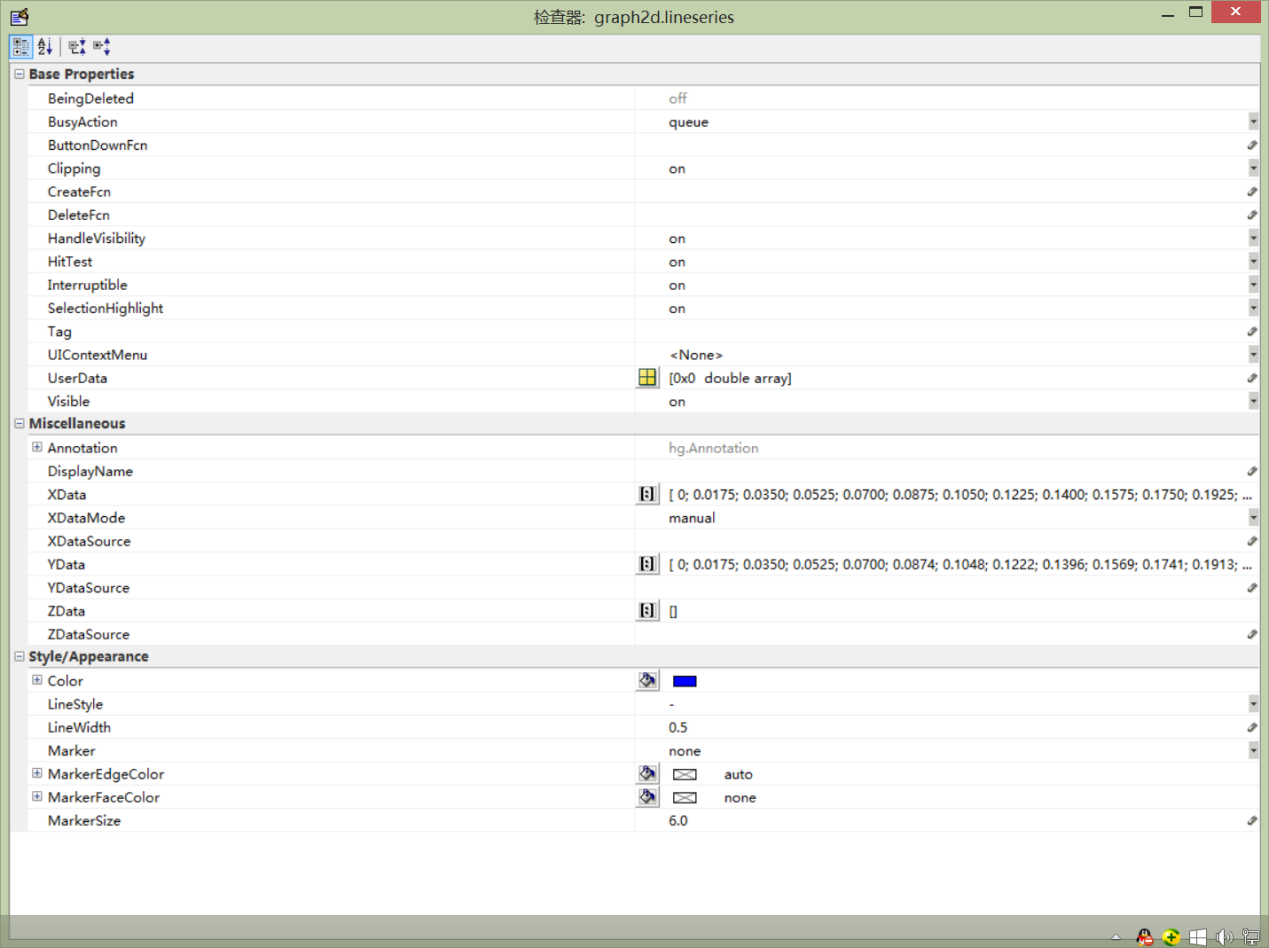
\includegraphics[height=4cm]{images/27.jpg}
        % \end{figure}
        % \textbf{3. Lineseries     Function line}
        % \begin{enumerate}
        %   \item Base properties
        %   \item miscellaneous\qquad 混杂的
        %     \begin{enumerate}
        %         \item Annotation\qquad 注释
        %         \item Display Name\qquad 数据名
        %         \item xDtata
        %         \item xDtataMode
        %         \item Function
        %         \item Granularity
        %         \item userArgs
        %     \end{enumerate}
        %        \item style/appearance  风格
        %         \begin{enumerate}
        %          \item Color
        %          \item Linestyle
        %          \item Linewidth
        %          \item Marker
        %          \item Marker Edgecolor
        %          \item Marker facecolor
        %          \item Allowed style
        %          \item Alpha
        %          \item Marker size
        %     \end{enumerate}
        % \end{enumerate}
        % \begin{figure}[H]
        % \centering
        % 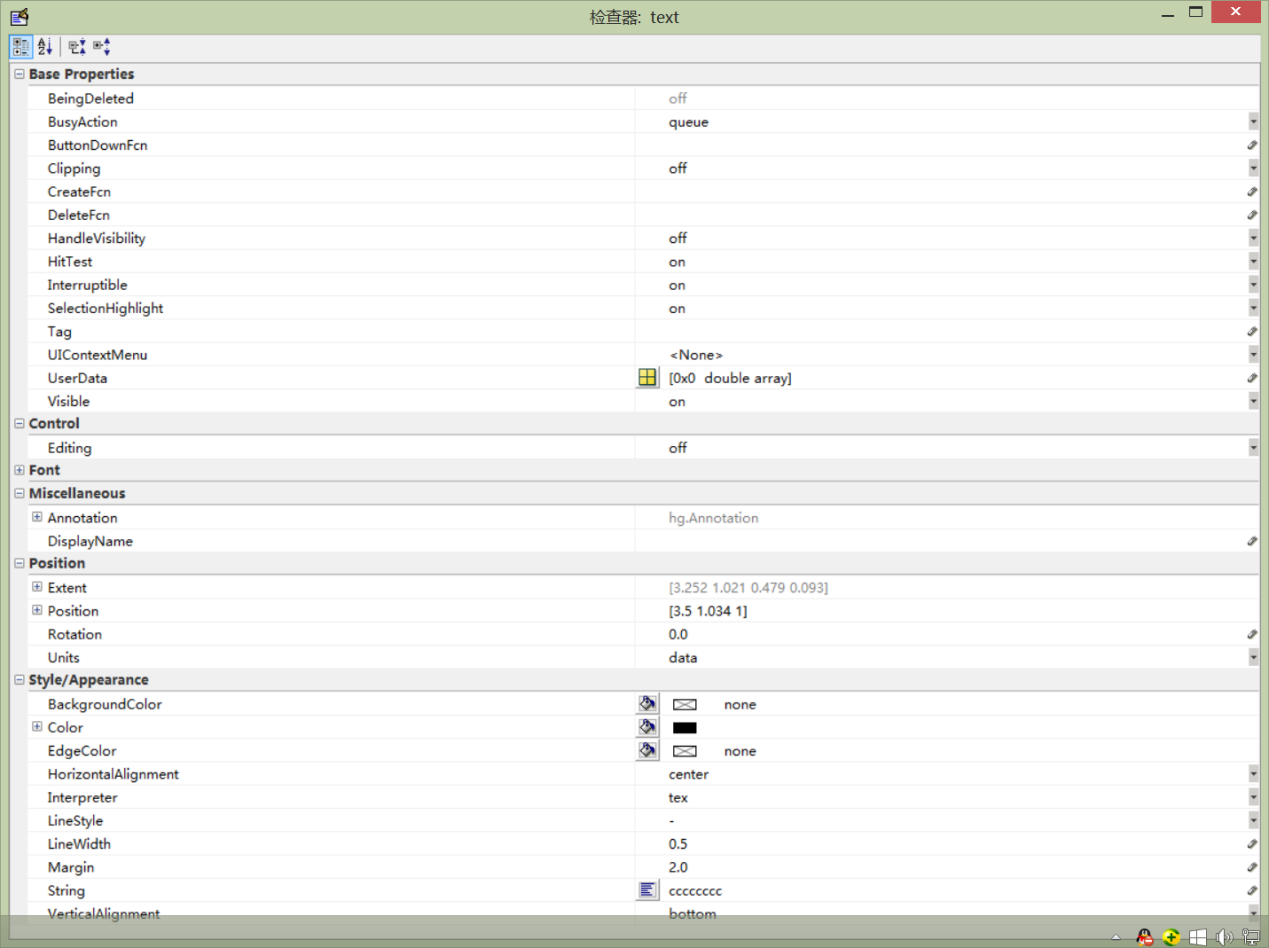
\includegraphics[height=4cm]{images/28.jpg}
        % \end{figure}
        % \begin{figure}[H]
        % \centering
        % 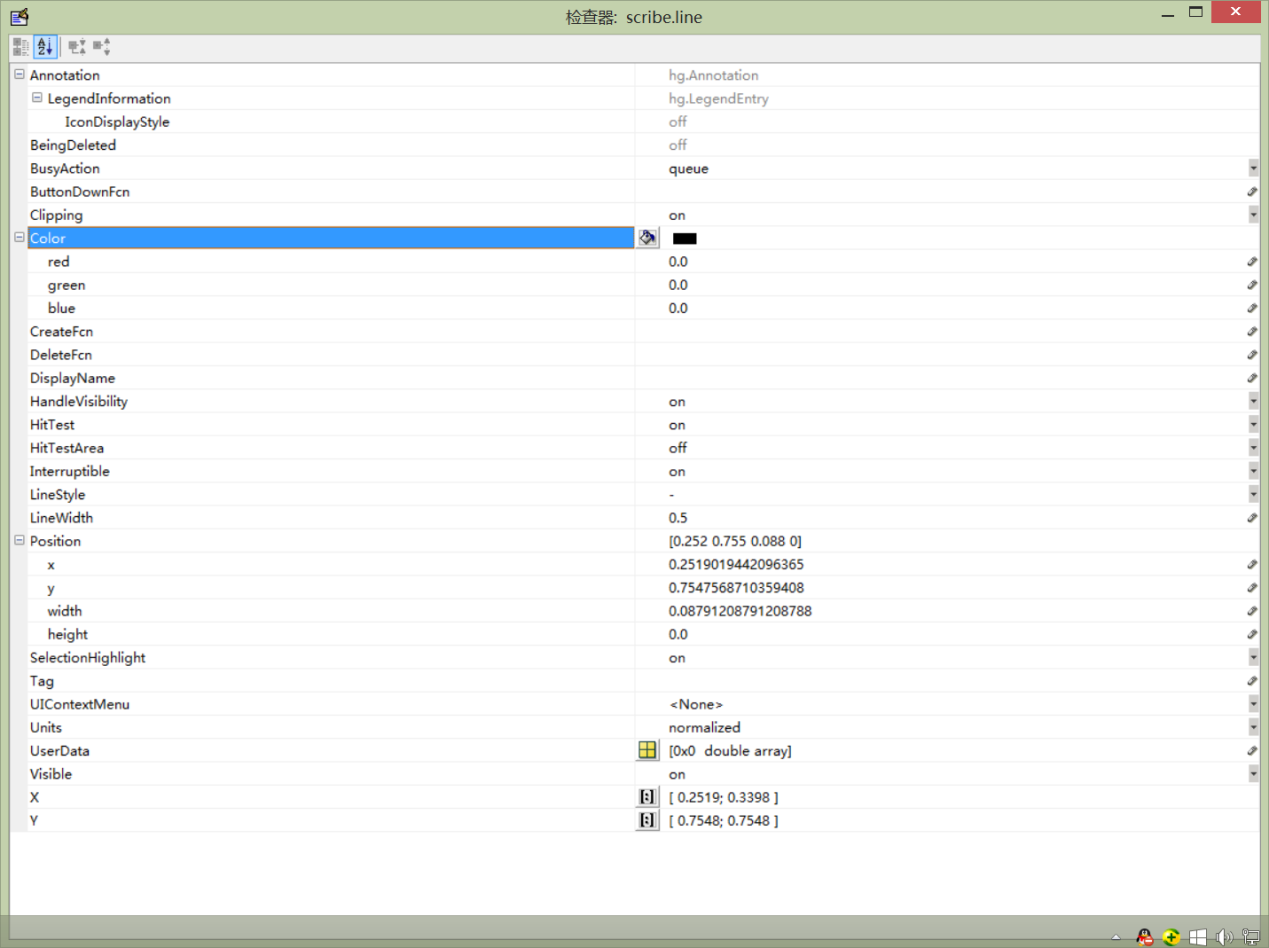
\includegraphics[height=4cm]{images/29.jpg}
        % \end{figure}
        % \begin{figure}[H]
        % \centering
        % 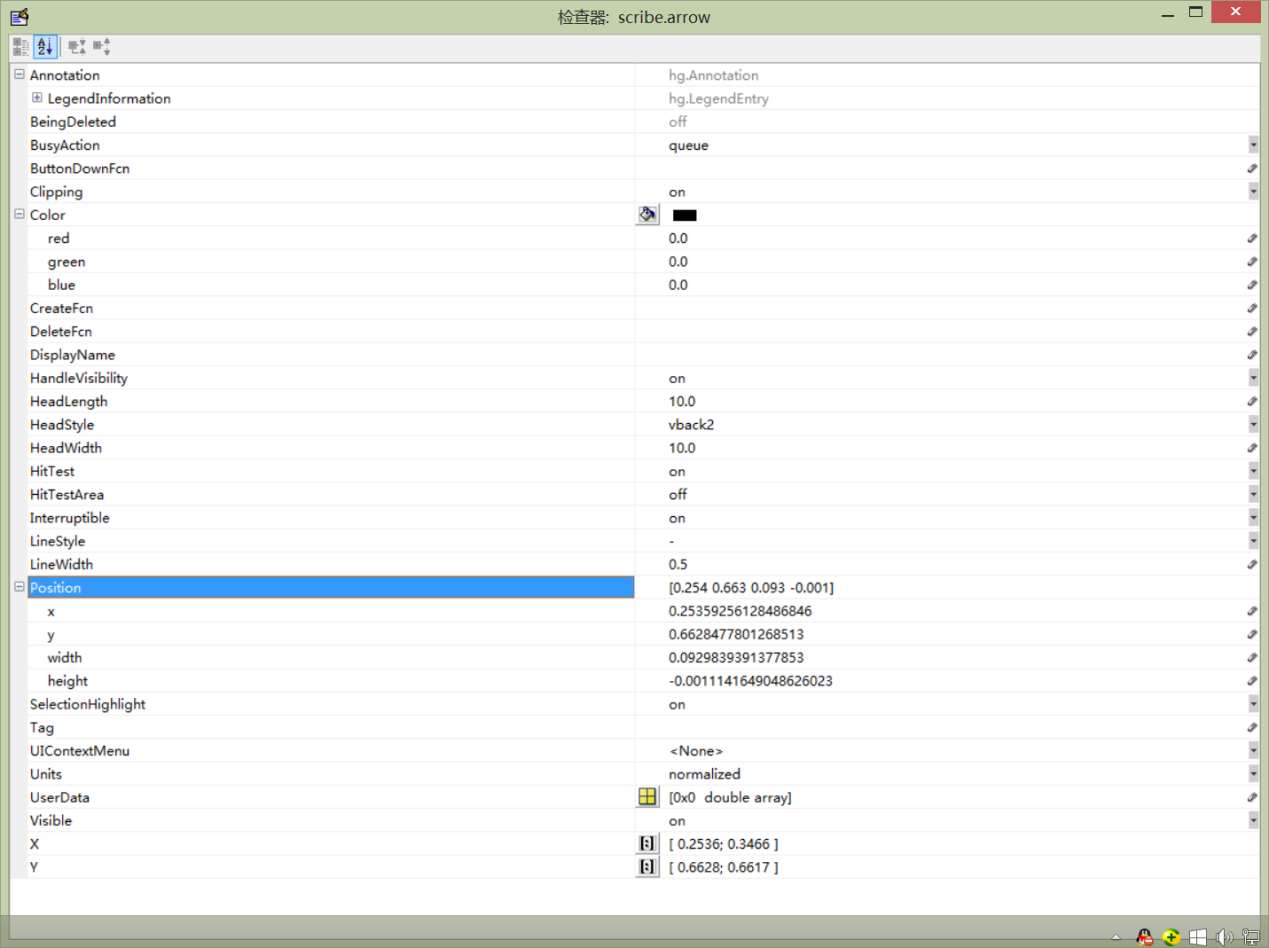
\includegraphics[height=4cm]{images/30.jpg}
        % \end{figure}
        % \textbf{4.Xlable ylable text}
        % \begin{enumerate}
        %   \item Base properties
        %   \item Control
        %   \item Font
        %     \begin{enumerate}
        %        \item fontangle\qquad 角度
        %         \item fontname
        %         \item fontsize
        %         \item fontunits
        %          \item fontweight
        %     \end{enumerate}
        %    \item miscellaneous\qquad 混杂的
        %    \item  position
        %     \begin{enumerate}
        %         \item extent(范围)x/y/width/height
        %         \item rotation(方向)
        %         \item units
        %         \end{enumerate}
        %    \item style/appearance
        %     \begin{enumerate}
        %         \item Color
        %         \item Edgecolor
        %         \item Backgroundcolor
        %         \item Horizontal Alignment(对齐方向—水平对齐)
        %         \item vertical Alignment(竖直对齐)
        %         \item Linestyle
        %         \item Linewidth
        %         \item Margin
        %         \item String
        %         \end{enumerate}
        % \end{enumerate}
        % \begin{figure}[H]
        % \centering
        % 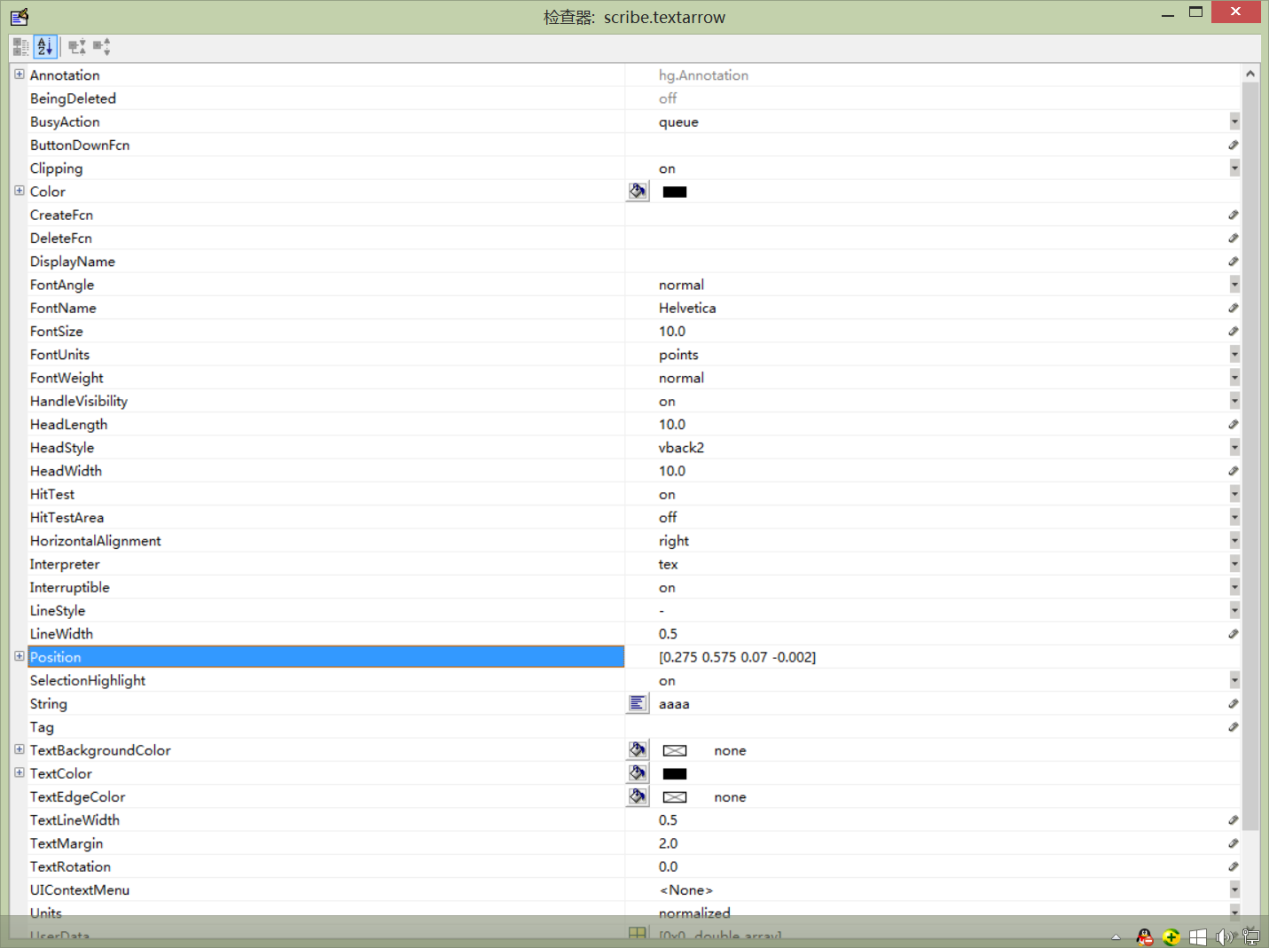
\includegraphics[height=4cm]{images/31.jpg}
        % \end{figure}
        % \textbf{5. Textbox}
        % \begin{enumerate}
        %        \item Color
        %         \item Edgecolor
        %         \item Backgroundcolor
        %         \item Fit box to text    on/off
        %         \item Handle visibility
        %         \item font
        %         \item Interpreter
        %         \item Linestyle
        %         \item Linewidth
        %         \item Margin
        %         \item Position
        %         \item Select hightlight   on/off
        %         \item String
        %         \item Horizontal Alignment(对齐方向—水平对齐)
        %         \item vertical Alignment(竖直对齐)
        % \end{enumerate}
        % \begin{figure}[H]
        % \centering
        % 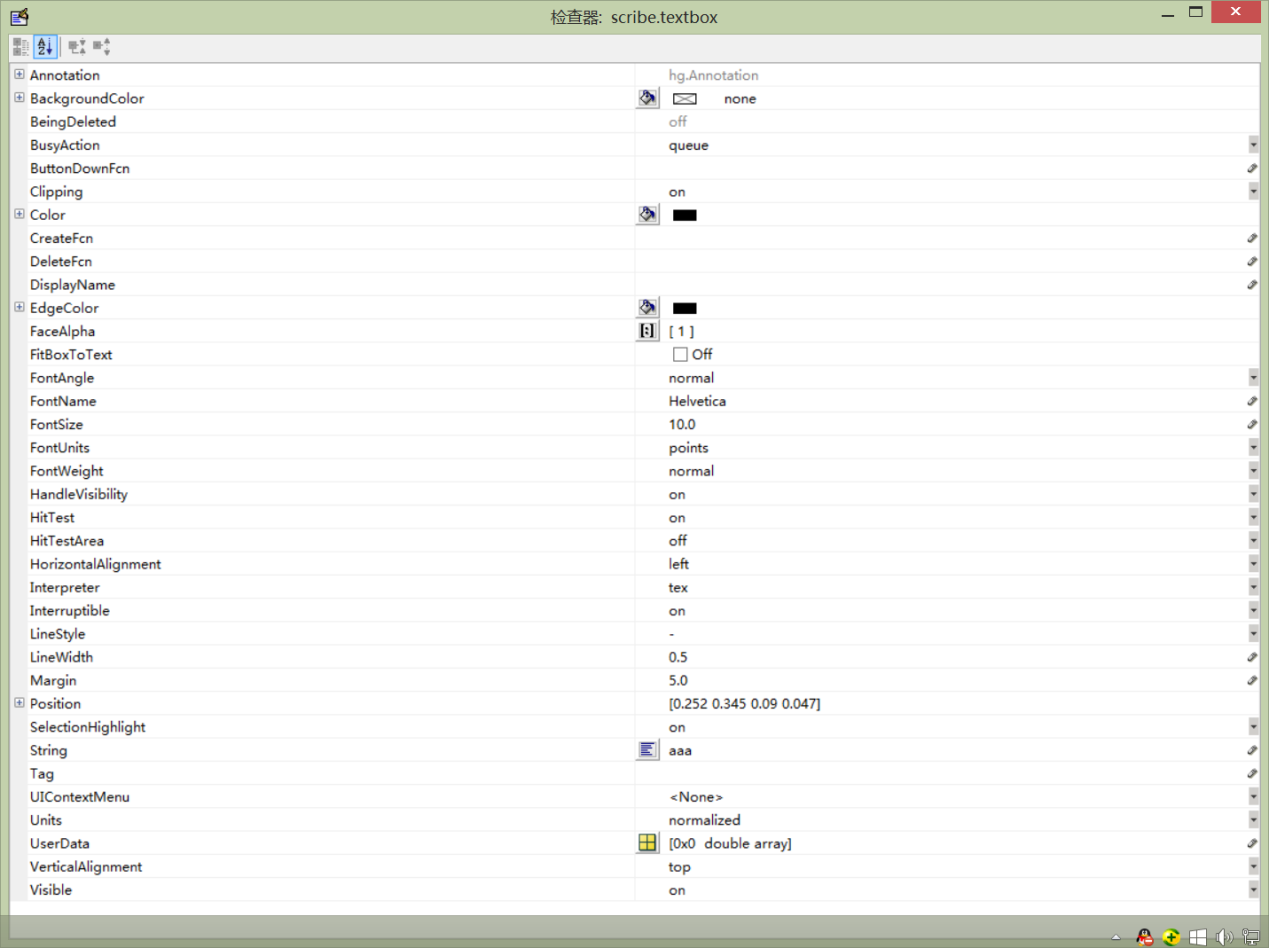
\includegraphics[height=4cm]{images/32.jpg}
        % \end{figure}
        % \textbf{6. scribe. scribe rect/ellipse}
        % \begin{enumerate}
        %        \item Color
        %         \item facecolor
        %         \item Linestyle
        %         \item Linewidth
        %         \item Position
        % \end{enumerate}
        % \textbf{7. line/arrow/double arrow/textarrow}
        % \begin{enumerate}
        %        \item Scribe
        %         \item Head lenghth
        %         \item Head style
        %         \item Head width
        %         \item Head length
        %         \item Head style
        % \end{enumerate}
        % \textbf{8. legend/scribe legend}
        % \begin{enumerate}
        %   \item Axes rules
        %   \item   Base properties
        %   \item Camera
        %   \item Color
        %   \item Control
        %   \item Font
        %   \item Miscellaneous
        %     \begin{enumerate}
        %        \item Edgecolor
        %         \item Textcolor
        %         \item Location
        %         \item string
        %         \item textcolor
        %         \item Interpreter
        %         \item Orientation: Horizontal Alignment(对齐方向—水平对齐)/vertical Alignment(竖直对齐)
        %     \end{enumerate}
        %   \item Position
        %   \item Style
        %     \begin{enumerate}
        %     \item Box  on/off
        %     \end{enumerate}
        % \item tick
        % \end{enumerate}
        % \begin{figure}[H]
        % \centering
        % 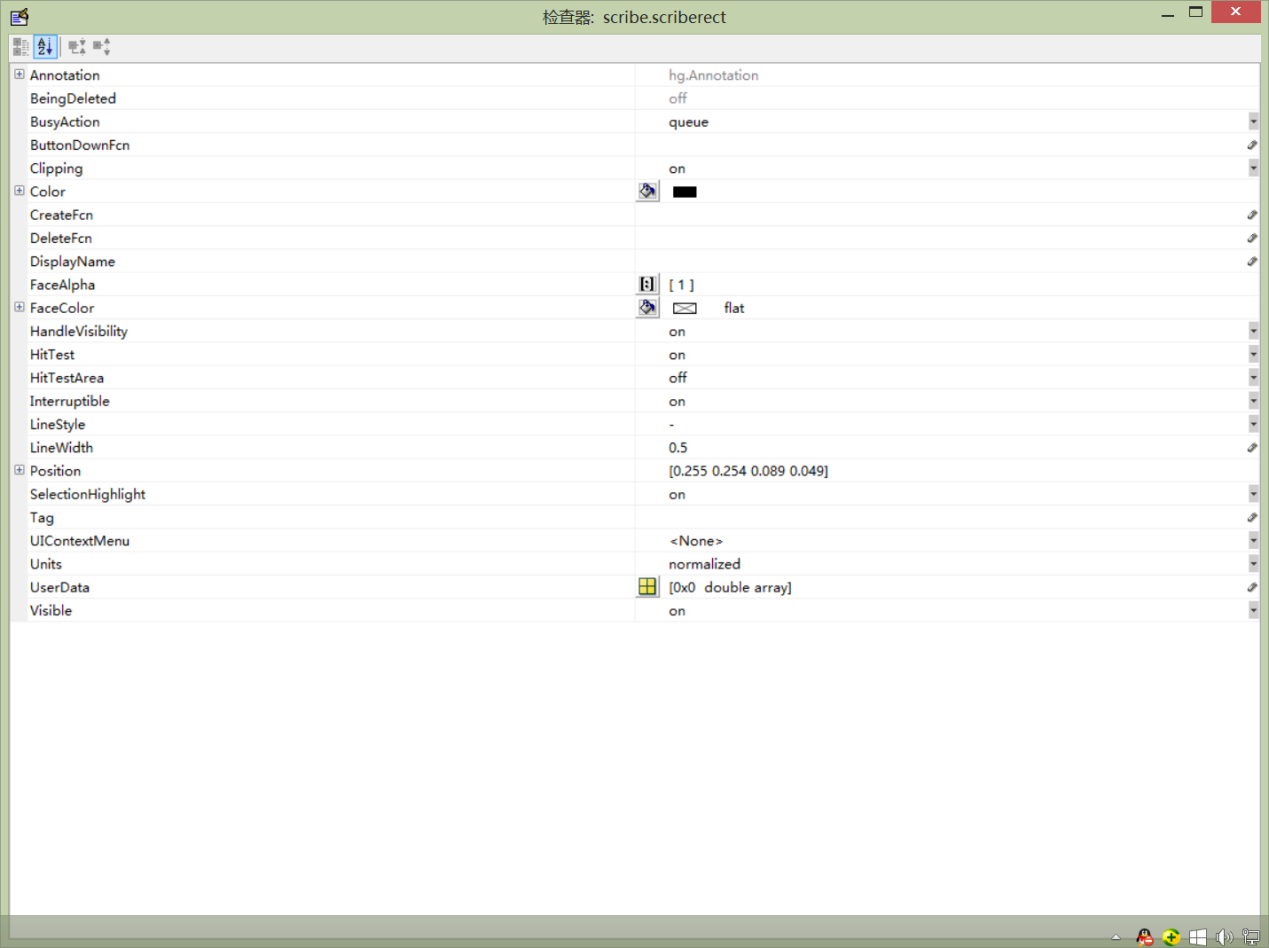
\includegraphics[height=4cm]{images/33.jpg}
        % \end{figure}
        \par
        最后我们来讨论如何获取和修改图形中对象的属性值,MATLAB通过handle类对象来对图形数据(属性值)进行访问\cite{xuxiao.2015}。
        \begin{lstlisting}[language=Matlab]
        h = figure              %将对象figure赋值给句柄类
        a = get(h, ’color’)     %得到对象/句柄h的‘color’属性的属性值
        b = set(h, ’color’, r)  %得到对象/句柄h的‘color’属性的属性值,颜色为红色
        \end{lstlisting}
        \par
        当然,如果一个图形没有设置figure对象时,仍然可以用get/set得到对象属性,因为其有默认的句柄:figure的默认为gcf;Axes的默认为gca;lineseries的默认为gcl。所以上面的操作也可以写为
        \begin{lstlisting}[language = Matlab]
        a = get(gcf, ’color’)
        \end{lstlisting}
        但要注意的是,当你打开多个图形窗口时,gcf为你正在操作的那个图形窗口(active)的figure。通过get/set的方法(handle类),你可以很容易的得到和设置某对象某属性的属性值。关于handle类get/set的方法,你可以参考文献\cite{xuxiao.2015}P50。
        % \par
        % \textcolor[rgb]{1.00,0.00,0.00}{引入:MATLAB是英文的吗?不是的,许多人再利用help .doc等帮助时发现其所给的帮助是英文的。这似乎使得入门的门槛较高。实际不是这样的,matlab是语言的,勤加使用你会发现,即使你的英语水平不高(像我六级在写本书就还没过),你也可以很快学会MATLAB。这就像我可以参考英文文献一样(我只看到了论文的思路与模型),其余的读不懂时再查英文也不迟,没必要咬文嚼字了。但不得不说的一点是,英文真的很重要,学好英文,对于我们的深入学习有很大的帮助,这是一个英语差生的一些感悟了。}
    \subsection{doc、demo and mathworks.com介绍}
        \par
        这一部分,我们将介绍如何快速高效的入门MATLAB。这里,向大家推荐几件神器doc、demo和mathworks.com。其中mathworks.com是doc和demo的网页版,并且你可以在mathworks.com上学习更多的知识。
        \par
        首先,我们来介绍第一神器doc。在command命令窗口输入doc命令即可打开该命令的帮助文档,这里的文档是相当详尽的。例如,我们输入doc plot会得到如图(\ref{doc help示意图}) 所示的帮助窗口,帮助窗口左边有帮助系统的目录,而右边提供了plot命令、Syntax(语法/用法)、description(描述)、output argunants (输出参数)、Moreabout(更多或拓展)、seealso(看了又看,同类/相关)。对于使用doc的matlab user而言,doc中的examples可能是最为重要。因为大部分人不喜欢读文字,所以,不如直接举个例子。而这对于想系统学习Matlab结构及matlab user而言,左边的contents是比较重要的,因为它可以给你一个M概况,而不是琐碎的细节。学MATLAB最好的老师就是Matlab自身了,它除了给你提供大量的帮助文档外,你还可以open function来观察matlab user是如何编写Matlab函数文件的,这样可以快速提高你的Matlab水平。
        \begin{figure}[H]
        \centering
        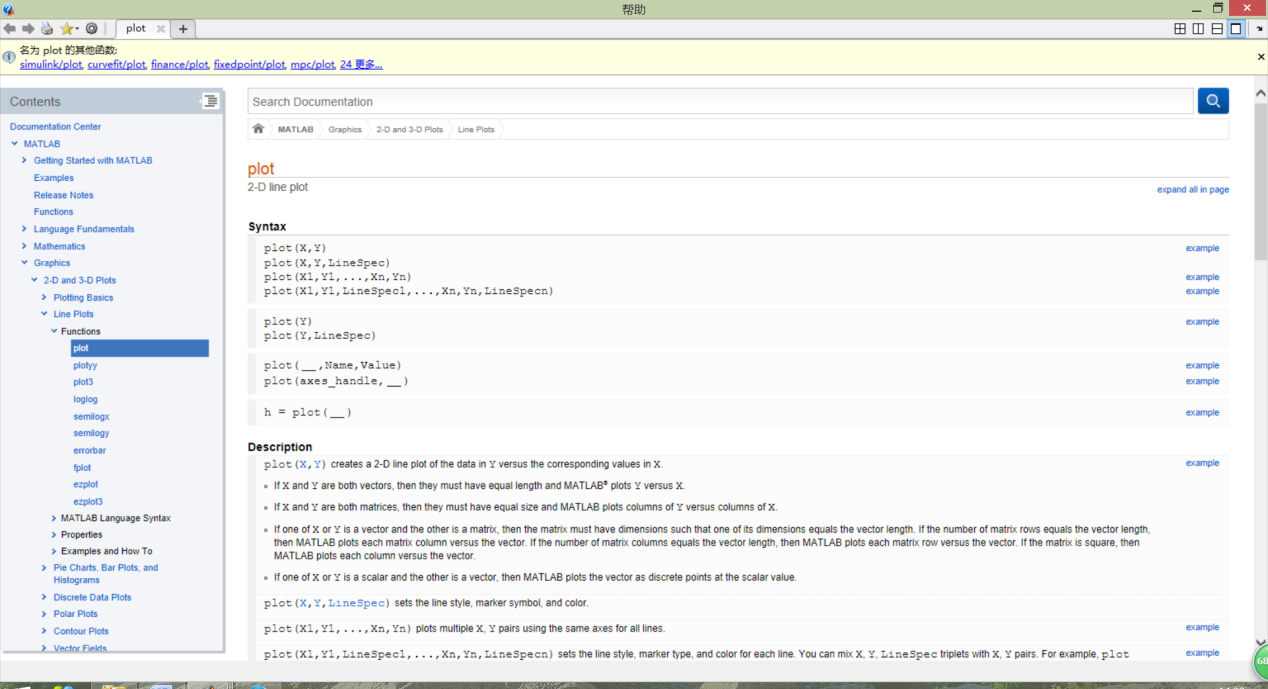
\includegraphics[height=8cm]{images/34.jpg}
        \caption{doc help示意图}
        \label{doc help示意图}
        \end{figure}
        \par
        其次,我们来看第二个神器demo。demo是帮助的拓展,你可以发现,在MATLAB安装目录的toolbox下,几乎每个工具箱都有一个*demos文件夹。这里面存放着该工具箱的演示用品(用于演示如何使用工具箱),包括:Matlab脚本、Matlab函数、Matlab.dat数据以及其它所需。当然,这些文件你也可以在mathworks.com的产品—工具箱—代码示例中看到。
        \par
        我们来看一下statistic和机器学习toolbox的演示文档
        \begin{lstlisting}[language = Matlab]
        doc demo
        demo toolbox statistic
        \end{lstlisting}
        statistic toolbox的演示文档如图(\ref{fig:statistictoolbox的演示文档})所示。可以看到的是demo给出了该toolbox的用法(.doc给出某命令的用法),这使得你能够很快入门MATLAB的toolbox。演示文档上的MATLAB脚本文件不需要复制粘贴,它们已经位于该toolbox的demo文件夹中。
        \begin{figure}[H]
        \centering
        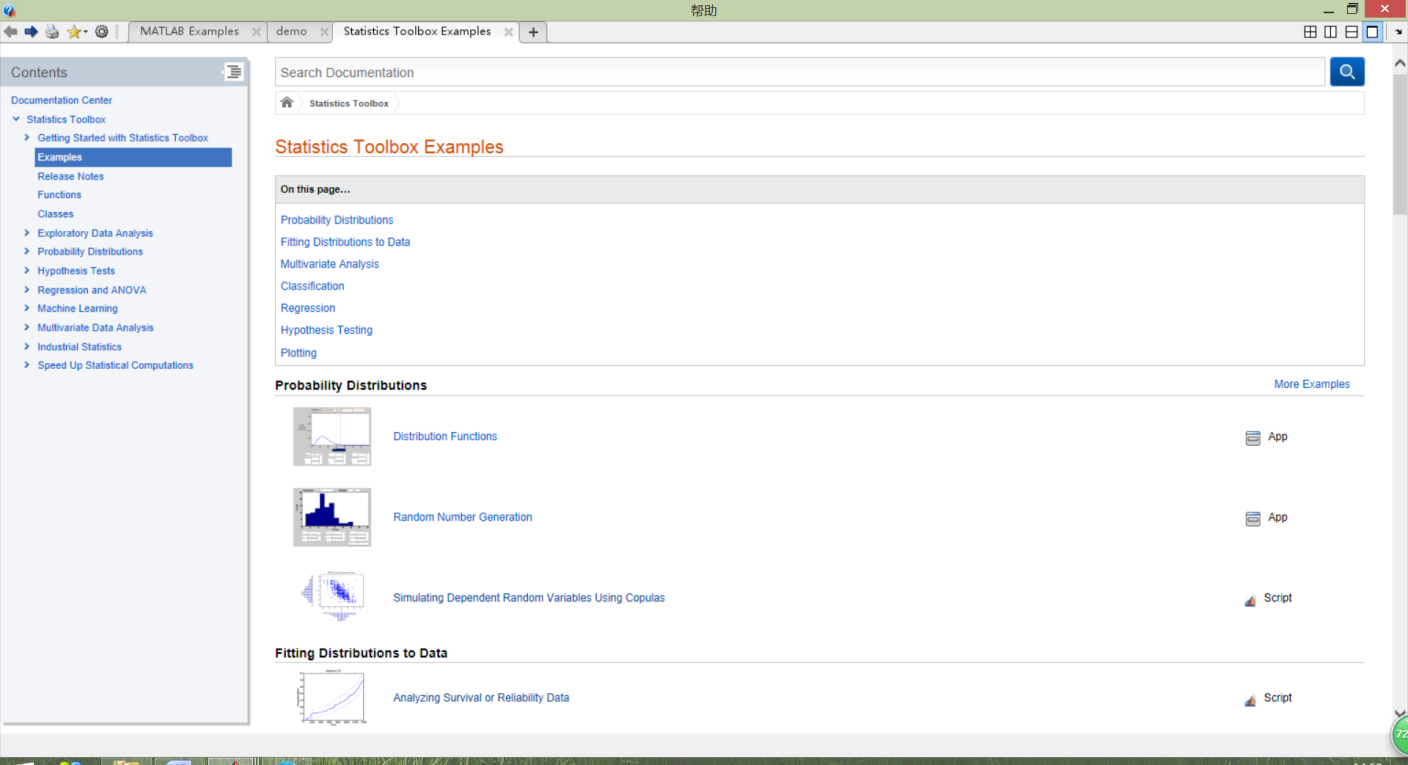
\includegraphics[height=8cm]{images/35.jpg}
        \caption{statistictoolbox的演示文档}
        \label{fig:statistictoolbox的演示文档}
        \end{figure}
        \par
        最后,我们来介绍第三个神器:mathworks.com。mathworks.com是需要经常浏览的一个网站,在学习MATLAB的过程中,我们会发现这个官网是多么的重要与详尽。有时候,我们想看某些学科的MATLAB操作(如上面demo中的统计与机器学习的内容)。但是打开MATLAB进入demo学习是非常不容易的,因为:\ding{172}MATLAB打开很耗时,也耗内存;\ding{173}demo只提供你安装版本MATLAB toolbox的演示文档,你并不知道高版本MATLAB toolbox引入了哪些新技术。所以,更多学习是在mathworks.com中进行的。mathworks.com官方网址是:\url{http://cn.mathworks.com/}。此时点击进去,会发现MATLAB的新技能Hadoop、深度学习Deeplearn,如图(\ref{mathworks官网})。此外,在浏览MATLAB网页时,有几个比较不错的去处:
        \par
        $\heartsuit\text{Love MATLAB \& MATLAB Sky}$
        \par
        $\heartsuit\text{知乎MATLAB专栏}$
        \par
        $\heartsuit\text{关注Mathworks的官方微博}$
        % \par
        % \textcolor[rgb]{1.00,0.00,0.00}{留白以补充:1.mathworks.com的支持—微博下有大神们的M作品,全都非常漂亮!
        % 2.A new tool—实时编辑器\footnote{http://cn.mathworks.com/products/new products/latest features.html?s tid=hp spot R2016a 0316-- MATLAB产品的更新}};
        \begin{figure}[H]
        \centering
        
\includegraphics[height=8cm]{images/36.jpg}
        \caption{mathworks官网}
        \label{mathworks官网}
        \end{figure}
    \subsection{MATLAB常用绘图命令}
        \par
        \cite{zhangdefeng}一书很详实的介绍了大部分绘图命令,可以作为参考。虽然前面介绍了图形的GUI操作,但作为一门语言,我们更倾向于用命令程序的方式来绘制修饰图形。我们整理了大部分图形命令,并列举了常用的绘图命令以及它们的具体方法。详细的Matlab绘图命令可以在mathworks.com查询。MATLAB更是提供了pdf格式文件来展示,网址\footnote{http://cn.mathworks.com/help/pdf doc/matlab/index.html}下的pdf 格式说明文档\footnote{http://cn.mathworks.com/help/pdf doc/matlab/graphg.pdf}。另外有类似demo、doc的网址,如网址\footnote{http://cn.mathworks.com/help/matlab/index.html}下的内容\footnote{http://cn.mathworks.com/help/matlab/graphics.html}相当于doc命令帮助窗口。在此处,你可以浏览整个绘图命令,也可以查找具体命令的具体用法类似(doc)。当然,这里提供的是最新版本MATLAB的命令情况。
        \par
        下面,我们列举一些常用的绘图命以及一些常用的图形修饰命令,更全面的绘图命令你可以在网址\footnote{http://cn.mathworks.com/help/matlab/functionlist.html graphics}下的图形函数list中查看。
        \par
        绘制2D图像常用的函数:
        \begin{lstlisting}[language = Matlab]
        plot(x1,y1,x2,y2,linesapce,’name’,’value’)% 点线图
        plotyy(x1,y1,x2,y2,’plot’,’hist’)% 用plot绘左轴,hist绘右轴的等轴曲线图
        line(x,y,’name’,’value’)% 点线图
        ezplot(func)% func可以是incline函数[xmin,xmax,ymin,ymax]
        fplot% 函数图
        \end{lstlisting}
        \par
        1、2、4、5命令的syntax中有linespec参数,其表示线的颜色、标号、线型
        例如,我们用’ro-’表示该线是’r’红色;’o’线上点的标号用’o’;’-’连接各点线的类型是实线,表(\ref{tab:linespace常用图形修饰函数})给出了linespace可供选择的3种属性的属性值,并介绍了一些常用的图形修饰函数(命令)。
        \begin{table}[H]
        \caption{linespace常用图形修饰函数}
        \label{tab:linespace常用图形修饰函数}
        \centering
        \begin{tabular}{c l c l}
            \toprule
            命令 & 说明 & 命令 & 说明 \\
            \midrule
            title & 在当前坐标轴上添加标题 & hold on & 添加新绘图时保留当前绘图\\
            xlabel & 为x轴添加标签      &subplot & 在平铺位置创建坐标轴\\
            ylabel & 为y轴添加标签     &text  & 向数据点添加文本说明\\
            legend & 将图例添加到图表&texlabel   & 将文本格式化为 TeX 字符串\\
            colorbar & 显示颜色标度的颜色栏&cla & 清除坐标轴\\
            xlim & 设置或查询x轴范围&daspect & 控制沿每个轴的数据单位长度\\
            get & 查询图形对象属性&pbaspect  & 控制每个轴的相对长度\\
            set & 设置图形对象属性&clear fig & 清除图形窗口\\
            box on  & 显示坐标轴轮廓&hidden on & 透视\\
            grid on & 显示或隐藏坐标轴网格线&gtext & 在图形窗口点击位置,在该位置上显示str\\
            \bottomrule
        \end{tabular}
        \end{table}
\section{MATLAB的一些杂例 }
    \par
    这一章节更多的介绍了一些新版本中的绘图命令以及一些统计绘图的例子。
    MATLAB的绘图工具箱在2014b版时发生了一些较大的变化,这些变化你可以在网址\footnote{http://cn.mathworks.com/help/matlab/release notes.html}上找到。\\
    \textbf{1.可旋转的tick lables}
    \par
    在给坐标轴的刻度添加lables时,如果lable文本过长,会给工作增加许多麻烦,因为在2014b版本之前,MATLAB允许的tick lables只有两个方向:垂直与水平。它不支持labels任意角度的旋转。在2014b之后,MATLAB允许tick lable任意角度旋转(当然,2014b之前,已经有人开发了tick lables旋转这个命令)。
    \begin{lstlisting}[language=Matlab]
    ax = gca;
    ax.xtickLableRotation = -35;      %顺时针旋转35度
    \end{lstlisting}
    \textbf{2. 2014b引入新函数:histogram(创建两个重叠直方图并修改其属性)}
    \begin{lstlisting}[language=Matlab]
    data1 = randn(5000,1);
    data1 = randn(5000,1) + 2;
    h1 = histogram(data1);      %doc histogram
    hold on
    h2 = histogram(data2);      %2015b引入 histogram2
    hold off
    legend show
    h1.Binmethod = ‘sturgcs’;
    h2.Normalization = ‘countdensity’;
    \end{lstlisting}
    \textbf{3. 2013a引入新函数yyaxis}
    \begin{lstlisting}[language=Matlab]
    Doc yyaxis
        yyaxis left
        yyaxis right
        yyaxis(ax……)
    x = linespace(0, 10);
    y = sin(3*x);
    yyaxis left
    plot(x,y)
    z = sin(3x).*exp(0.5x);
    yyaxis right
    plot(x, z)
    ylim ([-150, 150])
    title, xlable, ylable
    yyaxis left
    ylable()
    ax = gca;
    yyaxis left
    ax.Ydir = ‘reverse’;
    ax.YAxis(1).Direction = ‘reverse’;
    ax.Ycolor = RGB
    \end{lstlisting}
    \textbf{4. Bubbleplot可以绘制多维数据}\\
    \textbf{5. 气泡图BubbleGum.m}\\
    \textbf{6. stackedbar3绘制三维堆积柱状图}
    \par
    利用MATLAB自带命令bar3只可以绘制三维bar,虽然可以进行堆积操作stacked(bar中有堆积操作),但是此堆积只有一个维度的堆积。
    \begin{lstlisting}[language=Matlab]
    load count.dat
    Y = count(1:10, :)
    bar3 (y, ’stacked’)
    \end{lstlisting}
    值得庆幸的是,有一个stackedbar3函数可以解决3维堆积情况,该函数的用法如下
    \begin{lstlisting}[language = Matlab]
    h = stackedbar3(array);
    ax.projection = ’ projection’;
    ax.Grid = 10n’;
    \end{lstlisting}
    \textbf{7. fillbetween填充两个图之间的部分}\\
    \textbf{8. fplot,fsurf,fmesh,fcountour,fplot3于R2016a升级}\\
    注:对于axes而言,axis = axes is\\
    \ding{172}fplot(R2016a)语法(syntax)如下
    \begin{lstlisting}[language = Matlab]
    fplot(f)
    fplot(f,xinterval)
    fplot(xt,yt,tinterval)
    fplot(_,linespec)
    fplot(_,name,value)
    \end{lstlisting}
    其应用示例如下:
    \begin{lstlisting}[language=Matlab]
      fp = fplot(@(x),sinx,[-2pi,2pi],'-.*c','linewidth',2)
      fp.linestyle = ‘-’;
      grid on
      ax = gca;
      ax.xTick = -2*pi:pi/2:2*pi
      ax.xTickLable = {'-2 /pi','-3\pi/2','-/pi','O','\pi/2','1\pi','-3\pi/2','-2 /pi'}
    \end{lstlisting}
    \ding{173}fplot3语法如下
    \begin{lstlisting}[language = Matlab]
    fplot3(xt,yt,zt,tinterval)
    fplot3(_,linespec)      %线的形状、颜色、标号
    fplo3t(_,name,value)
    \end{lstlisting}
    \par
    用其绘制如下函数图象
    \begin{equation*}
    \centering
    \left\{\begin{lgathered}
    x=e^{\frac {|t|}{10}}\sin(5t)\\
    y=e^{\frac {|t|}{10}}\cos(5t)\\
    z=t
    \end{lgathered} \right.
    \end{equation*}
    绘制程序如下
    \begin{lstlisting}[language=Matlab]
    xt = @(t)exp(-t/10).*sin(5*t);
    yt = @(t)exp(-t/10).*cos(5*t);
    2t = @(t)t;
    fp3 = fplot3(xt,yt,zt,[-10,10],’linewidth’,1);
    fp3
    fp3.color = ’r’;
    \end{lstlisting}
    \ding{174}fsurf的语法如下
    \begin{lstlisting}[language = Matlab]
    fsurf(f, xyinterval)
    fsurf(funx, funy, funz, uninterval)
    fsurf(_, linespec)
    fs = fsurf(_, name, value)
    \end{lstlisting}
    \ding{175}fmesh与fsurf几乎相同。\\
    \ding{176}fcountour例子可以用fsurf的例子\footnote{补充pie3的用法}。\\
    \textbf{9. MATLAB图形对象及更新(R2014b)}
    \par
    MATLAB2014b之后,我们可以使用下面的方法来查看绘图对象
    \begin{lstlisting}[language=Matlab]
    p = plot(x,y);
    p                     %返回line对象
    who p
    p.color = ’r’;        %P对象可以使用点符号(‘.’,即dot index)进行取值与赋值
    \end{lstlisting}
    而在R2014b之前,我们如此设置
    \begin{lstlisting}[language=Matlab]
      set(p, ’color’, ’r’);
      get(p)              %返回p对象所有属性
      set(p, ’linestyle’) %查看p对象linestyle属性的可选属性值
    \end{lstlisting}
    \textbf{10. MATLAB R2014b之后的图形变的更加平滑}
    \par
    旧版本的MATLAB图不是很光滑,总感觉断断续续的。老版本绘图如图(\ref{绘图光滑示意图1})所示,新版本绘图如图(\ref{绘图光滑示意图2})所示
    \begin{figure}[H]
    \centering
    \begin{subfigure}[b]{0.4\textwidth}
        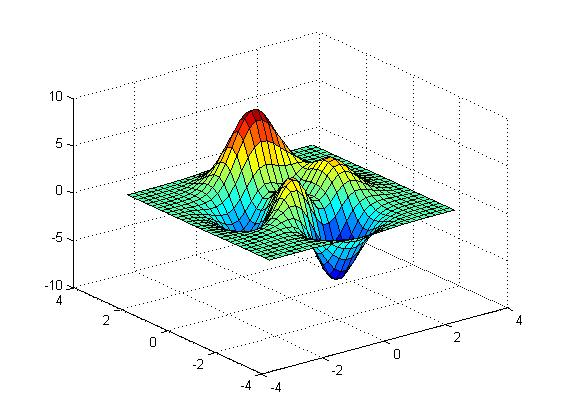
\includegraphics[width=\textwidth]{images/43.jpg}
        \caption{}
        \label{绘图光滑示意图1}
    \end{subfigure}
    \begin{subfigure}[b]{0.4\textwidth}
        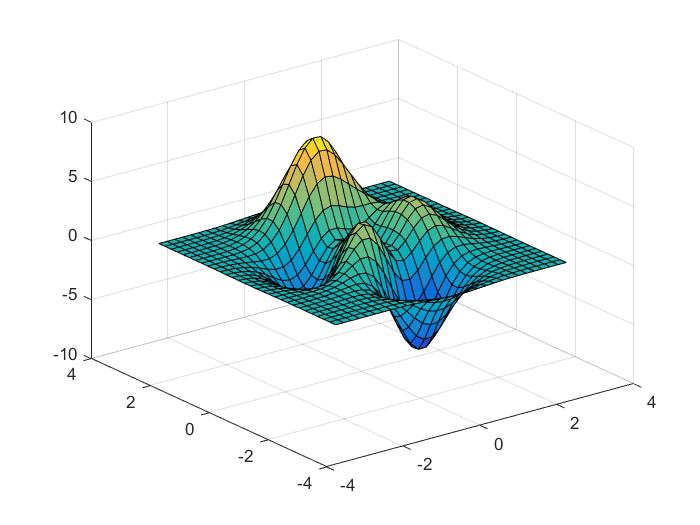
\includegraphics[width=\textwidth]{images/42.jpg}
        \caption{}
        \label{绘图光滑示意图2}
    \end{subfigure}
    \caption{绘图光滑示意图}
    \end{figure}
    \par
    R2014b图形的title、xlable默认字体大小比之前要更大;R2014b之后colorbar and legend no longer Axes,而是colorBar对象;R2014b之后的bar、contour、stem也已经改变为hggroup对象
    \begin{lstlisting}[language=Matlab]
      findobj(’type’, Axes)    %不再返回colorbar & legend
    \end{lstlisting}
\chapter{MATALB数据结构}
\section{MATLAB操作命令}
    \par
    下面的许多表格中,有部分命令是没有说明的(空白),需要读者自行查找填写。
    \subsection{有关命令窗口的操作}
        \begin{table}[H]
        \newcolumntype{Y}{>{\centering\arraybackslash}X}% 定义自适应列的居中格式 Y, 用 X 为左对齐(自适应列)
        \begin{tabularx}{\textwidth}{cXcX}% 需要引入 tabularx 宏包;表格总宽度一定要设置
            \toprule
            命令 & 语法说明 & 命令 &语法说明\\
            \midrule
            clc & 清除命令行 & save name & 保存工作空间变量到name.mat\\
            clear & 从工作空间清除所有变量 &save name x y & 保存工作空间变量x y到name.mat\\
            clear all  & {} & load & 从文件中读入变量 \\
            clear * & 清除*变量 & load name x y & {}\\
            cla & 清空当前坐标轴内容 & quit(或exit) & 退出MATLAB环境 \\
            clg & {}& startup & MATLAB自启动文件 \\
            clf & 清除图形窗口内容 & ! dos & {} \\
            close & 关闭打开的文件 & ctrl+c&终止正在运行的程序 \\
            close figure & {}& * + tab键 & {} \\
            more off & 不允许分页 & shift + tab键 & {} \\
            more on & 允许分页 & Beep & 发出声音\\
            more(n) & 指定每页输出行数 & Waitforbuttonpress & {}\\
            diary on&创建日志,默认文件名称为diary.txt & matlabroot&返回根目录\\
            diary off&结束日志&matlabrc & 启动主程序 \\
            diary *&创建名称为*.txt的日志 & yesinput & {}\\
            echo&显示文件中的MATLAB命令 & cedit & 设置命令行编辑与回调的参数\\
            diary *.m & 中断正在执行的命令 &help & 查询命令的帮助信息\\
            helpdesk & 打开超文本形式用户指南(浏览器模式)& lookfor & 对help信息中的关键词查找\\
            Doc & {} & Demo & {} \\
            \bottomrule
        \end{tabularx}
        \end{table}
        \noindent 注:1、ctrl+c可以在程序运行的任何时间暂停,并保存当前计算进度。但是它只能保存暂停处的函数所使用的局部变量,调用这个函数的函数剧本变量无法得知。
        \par
        2、more + 回车键前进一行、more + 空格键显示下一页、more + q终止当前显示。
    \subsection{常用快捷键 }
        \begin{table}[H]
        \centering
          \begin{tabular}{ccl}% 需要引入 tabularx 宏包;表格总宽度一定要设置
            \toprule
            功能键&快捷键& 功能说明\\
            \midrule
            $\uparrow$ & Ctrl+p &调出前一个输入的命令\\
            $\downarrow$ & Ctrl+n&调出后一个输入的命令\\
            $\leftarrow$ & Ctrl+b&光标左移一个字符\\
            $\rightarrow$ & Ctrl+f& 光标右移一个字符\\
            Home &Ctrl+a & 光标移至首行\\
            End& Ctrl+e&光标移至行尾\\
            Esc & Ctrl+u&清除当前行\\
            Del & Ctrl+d&清除光标所在位置后面的字符\\
            Backspace & Ctrl+h & 清除光标所在位置前面的字符\\
            Enter & {} & 前进一行\\
            {} & {} & 显示下一页\\
            {}&Ctrl+k&删除到行尾\\
            {}&Ctrl+c&中断正在执行的命令\\
            \bottomrule
        \end{tabular}
        \end{table}
    \subsection{文件操作语句}
        \begin{table}[H]
            \newcolumntype{Y}{>{\centering\arraybackslash}X}% 定义自适应列的居中格式 Y, 用 X 为左对齐(自适应列)
          \begin{tabularx}{\textwidth}{lllX}% 需要引入 tabularx 宏包;表格总宽度一定要设置
            \toprule
            命令 & 函数说明 & 命令 & 函数说明 \\
            \midrule
            getenv  &  获得环境参数 & fprintf & 将格式化数据写入文件,为 $x$ 轴添加标签 \\
            unix  &  执行操作系统命令并返回结果&  fgetl & 读取文件行并放弃换行符\\
            fopen  &  打开文件 fclose关闭文件  &fgets & 读取文件行并保持换行符\\
            tempname  &  建立临时的文件名  &ferror & 查询文件输入/出的错误信息\\
            tempdir  &  返回一个已存在的临时目录名 &feof&  检查文件结束标志\\
            fread  &  从文件中读取二进制数据&  fseek  &设置文件位置指针\\
            fwrite  &  向一个文件写二进制数据 &ftell   & 得到文件位置指针的位置\\
            fscanf  &  从文件读取格式化数据 & prewind   & 反绕一个打开的文件\\
            \bottomrule
            \end{tabularx}
          \end{table}
        \noindent 注:fprintf 可以决定数据的根本格式(即非显示格式)。
    \subsection{数据变量/文件}
          \begin{table}[H]
            \centering
          \begin{tabular}{llll}% 需要引入 tabularx 宏包;表格总宽度一定要设置
            \toprule
            命令 & 函数说明&命令 & 函数说明\\
            \midrule
            who  &  简要列出工作空间变量&size  &查询矩阵的维数\\
            whos  &  详细列出工作空间变量名&type *.m  &在工作空间查看*.m文件内容\\
            what   & 列出当前目录下的m文件和mat文件&delete  &从磁盘删除指定文件\\
            which &查找函数与文件所在的路径&disp  &{}\\
            dir &列出当前目录的内容&cell disp&{}  \\
            pack  &整理工作空间的内存&{} &\\
            \bottomrule
            \end{tabular}
          \end{table}
    \subsection{有关工作路径设置的命令}
        \begin{table}[H]
        \centering
          \begin{tabular}{llll}
            \toprule
            命令 & 函数说明&命令 & 函数说明\\
            \midrule
        cd或ls  &改变当前的工作目录&userpath  &修改工作路径\\
        cd () &修改目录(work文件夹)&savepath  &保存工作路径\\
        cd ..  &显示上一层目录&pathtool  &搜索路径管理器\\
        md(或mkdir)  &创建文件夹&addpath &增加文件搜索路径\\
        pwd &显示当前目录&genpath &将目录下的所有子目录都增加到路径中\\
        path  &查看matlab的搜索路径&rmpath  &去除文件搜索路径\\
        \bottomrule
        \end{tabular}
        \end{table}
        \noindent 注:1、cd是设置matlab的默认路径(目录)即matlab启动程序,在toolbox或load 下修改文件matlab rc.m,在其最后加上cd路径。
        \par
         2、addpath * -begin 添加路径*到搜索路径顶端。
    \subsection{数据显示格式}
        \begin{table}[H]
        \centering
        \begin{tabular}{ll}% 需要引入 tabularx 宏包;表格总宽度一定要设置
            \toprule
            命令 & 意义\\
            \midrule
        format short(默认)  &实数,用5位数字的科学计数法显示\\
        format short e  &5位科学计数法显示\\
        format short g  &从format short和format short e 中自动选择最佳计数方式\\
        format long &15位数字表示\\
        format long e &15位科学计数法表示\\
        format long g &从format long和format long e 中自动选择最佳计数方式\\
        format rat  &近似有理数表示(小数分数表示)\\
        format hex  &十六进制表示\\
        format $+$  &正数、负数、零分别用+、-、 空格\\
        format bank&  表示元、角、分\\
        format compact  &在显示结果之间没有空行的压缩格式\\
        format loose  &在显示结果之间有空格和空行的稀疏格式\\
        \bottomrule
        \end{tabular}
        \end{table}
        \noindent
        注:1、这里的数据显示格式并非保存格式,将其复制到EXCEL时仍为原格式。
        \par
         2、数据显示格式并非数据实质格式。

\section{MATLAB数据类型/对象}
    \subsection{矩阵matrix}
        \subsubsection{矩阵创建函数}
            \par
            \begin{table}[H]
              \newcolumntype{Y}{>{\centering\arraybackslash}X}% 定义自适应列的居中格式 Y, 用 X 为左对齐(自适应列)
            \begin{tabularx}{\textwidth}{lXlX}% 需要引入 tabularx 宏包;表格总宽度一定要设置
            \toprule
            函数 & 意义&函数 & 意义\\
            \midrule
            zeros &生成全零阵&eye  &生成单位矩阵 \\
             ones&生成 全1矩阵 &magic  &{}\\
            vander  &生成范德蒙矩阵&blkdiag& 产生以输入元素为对角线的矩阵\\
            compan& 生成友矩阵&cumprod &类似于sum\\
            hankel  &生成Hankel方阵&hilb  &生成Hilbert 矩阵\\
            invhilb&  逆Hilbert矩阵& pascal  &生成Pascal 矩阵\\
            hadamard  &{}&cat &创建多维数组\\
            randn &生成0~1间均匀分布的随机矩阵 &randperm& 产生1~n之间整数的随机排列\\
            linspace  &线性等分向量生成 &logspace & 生成对数等分向量\\
            strcmp  &字符串比较函数&findstr  &字符串查找\\
            strrep  &字符串替换函数 &sparse  &稀疏矩阵的创建\\
            full  &将稀疏矩阵转化为满矩阵& spconvert&  外部数据转化为稀疏矩阵\\
            find  &稀疏矩阵非零元素的索引& speye &创建单位稀疏矩阵\\
            spones  &创建非零元素是1的稀疏矩阵 &spdiags &创建对角或带状稀疏矩阵\\
            \bottomrule
            \end{tabularx}
            \end{table}
            \noindent
            注:1、$horcat \Leftrightarrow [A, B] \Leftrightarrow cat(1, A, B)$;
            \par
            2、$vercat \Leftrightarrow [A; B] \Leftrightarrow cat(2, A, B)$
        \subsubsection{常见的矩阵运算}
            \begin{longtable}{|c|l|c|l|}
            \hline
            \endfirsthead
            \multicolumn{4}{l}{(续表)}
            \endhead
            \hline
            \multicolumn{4}{c}{\itshape 接下页表格……}\\
            \endfoot
            \hline
            \endlastfoot
                \toprule
                 运算符 &  符号说明&运算符 &  符号说明\\
                \midrule
            A+B  &矩阵相加& rot90 &逆时针旋转90 度\\
            A*B &矩阵相乘 &flrplr &上下翻转\\
            A/B& 相除,左除还可以表示成inv(a)*b &flrpud  &左右翻转\\
            $A^k  $&矩阵的乘方运算 &flrpdim  &指定维数翻转\\
            det(A)  &向量的行列式 &shiftdim &元素移位\\
            rank(A) &向量的秩&  transpose &沿主对角线翻转矩阵\\
            trace(A)  &向量的迹 &circshift  &矩阵循环平移\\
            inv(A)  &矩阵的逆&  conv& 卷积\\
            pinv(A) &伪逆矩阵 &ceconv &反卷积\\
            expm(A) &方阵指数函数,这是一个内部函数  &kroon  &张量积\\
            sqrtm(A)  &矩阵的方根  &diag  &矩阵对角元素的抽取\\
            logm(A) &矩阵的对数,是lxpm(A)的反函数  &A.*B &{}\\
            eig &矩阵特征值与特征向量 &A./B &{}\\
            company &伴随矩阵&  $A.^k $&{}\\
            prod  &矩阵元素求积&  A’& transpose\\
            tril  &下三角阵抽取&  A.’ &ctranspose\\
            triu  &上三角阵抽取&  chol& 对称正定阵的Cholesky分解\\
            cross(A,B)  &向量的叉乘& lu& 矩阵的LU分解\\
            dot(A,B)  &向量的点积  &qr&  矩形矩阵的正交分解\\
            cond  &矩阵条件数  &schur  &方阵的舒尔分解\\
            reshape(A,2,6)& 矩阵重塑,将A变为2行6列 &svd  &{}\\
            repmat(A,m,n)&  矩阵的复制 &cholinc (chol)&{}\\
            polyvarm(P,A)&  矩阵的多项式& lu& luinc\\
            unm(A, $@$fun)& 计算矩阵A的函数  &union(A,B)&  两个集合的并集\\
            norm  &矩阵范数(维数较大时用normest)& unique(A) &不重复元素构成的向量\\
            poly  &{}&  blkdiag &{}\\
            meshgrid    &{}&  length&{}\\
            ndims   &{}&  numel &{}\\
                \bottomrule
            \end{longtable}
            \noindent 注:1.norm(A, 1)为1-范数,$||x||_1=|x_1|+|x_2|+\cdots+|x_n|$;
            \par
            2.norm(A, 2)为2-范数,$||x||2=(|x_1|^2+|x_2|^2+\cdots+|x_n|^2)^{1/2}$;
            \par
            3.norm(A, inf)为$\infty$-无穷范数,$||x||_\infty=\max(|x_1|,|x_2|,\cdots,|x_n|)$。

        \subsubsection{引入 - is判断函数}
            \begin{table}[H]
            \centering
              \begin{tabular}{llll}% 需要引入 tabularx 宏包;表格总宽度一定要设置
                \toprule
                 命令 &  说明&命令 &  说明\\
                \midrule
            issparse  &若是稀疏矩阵则为真  & isletter  &若是英文字母则为真 \\
            ismember& 检查是否属于指定集&isspace&  若是空格则为真\\
            isequal   &若两数组相同则为真&isempty  &若是空阵则为真\\
            isfield &若是构架域则为真&isglobal  &若是全局变量则为真\\
            ishandle&   若是图形句柄则为真&isfinite  & 全部元素都有限\\
            isieee &  计算机执行IEEE规则&isobject  &若是对象则为真\\
            ischar  &若是字符串则为真&  isprime   &若是质数则为真\\
            isnan &若是非数则为真& isreal  &若是实数则为真\\
            isinf &若是无穷数据则为真& isstudent &Matlab学生版规则\\
            isnumeric &若是数值数组则为真  &isscalar&  是否为标量\\
                \bottomrule
            \end{tabular}
            \end{table}
            \noindent 注:1、is a(x, ’数值类型’)
            \par
             2、is + tab键

        \subsubsection{常见统计函数}
            这里省略具体的例子,仅给出需要注意的几点。
            \begin{enumerate}
                    \item  round、floor、fix、roundn、ceil;
                    \item mod、rem;
                    \item 矩阵操作时,列优先;
                    \item 虚数表示为:z=a+bi=r*exp(i*theta);
                    \item exist(‘x’):查询工作空间中是否存在某个变量;
                    \item i=exist(‘x’):查询工作空间中是否存有’x’变量;
              \begin{enumerate}
                    \item i=0: 表示不存在以上变量和文件;
                    \item i=1: 表示存在一个变量名为’x’的变量;
                    \item i=2: 表示存在一个名为’x.m’的文件;
                    \item i=3: 表示存在一个变量名为’x.mex’的文件;
                    \item i=4: 表示存在一个变量名为’x.mdl’的文件;
                    \item i=5: 表示存在一个变量名为’x’的内部函数;
               \end{enumerate}
            \end{enumerate}

    \subsection{列表table}
        \par
        table类是MATLAB2013b新增的数据类型,类似于R语言中的dataframe数据类型。我们可以通过doc table在MATLAB上学习该数据类型,当然,如果你的MATLAB版本不允许的话(要求R2013b以上),可以通过下面网址\footnote{http://cn.mathworks.com/help/matlab/tables.html} 进行基本的学习。
        \par
        在研究后面的各种数据类型时,我们仅简单的介绍了数据类型的常用函数,以及某些小例子,对于数据类型的具体应用,将其放在了后面实战(建模)部分。
        \subsubsection{Table相关函数}
            \begin{table}[H]
            \centering
              \newcolumntype{Y}{>{\centering\arraybackslash}X}% 定义自适应列的居中格式 Y, 用 X 为左对齐(自适应列)
                \begin{tabularx}{\textwidth}{lXlX}% 需要引入 tabularx 宏包;表格总宽度一定要设置
                \toprule
                函数 & 意义&函数 & 意义\\
                \midrule
            Table   & 创建表数据类型&Readtable &从文件读取数据,创建表  \\
            Writetable  &将表写入文件&Istable &判断一个变量是否是table类型\\
            Height  &表的行数,返回table的高 & Width & 表变量的数量,返回table的宽\\
            Ndims   &返回table的维度&Numel  &返回table高和宽的乘积\\
            Horcat  &横向串接table&Vercat &纵向串接table\\
            Intersect &设置两个数组的交集&Ismember &数组的元素设置数组的成员\\
            Setdiff &设置两个数组的差&Setxor  &异或两个数组\\
            Unique  &独特的数组中的值&Union &设置两个数组联盟\\
            Join  &使用关键变量匹配行合并两个表&Innerjoin &内连接两个表\\
            Outerjoin &外连接两个表&Summary &描述表\\
            Sortrows  &排序数组的行,table按照制定的row排序&Stack &将多列堆成一列\\
            Unstack &一列展成多列 & Ismissing &找到没有赋值的项,返回logical index)\\
            StandardizeMissing  &给未赋值项赋默认值&Varfun &把函数作用在table中选定的变量上\\
            Rowfun  &应用函数表行& findgroups &发现组和返回组数字\\
            Splitapply  &数据分割成组织和应用功能&Table Properties  &访问和修改表元数据属性\\
                \bottomrule
            \end{tabularx}
            \end{table}
            \noindent 注:结构体struct可以是标量也可以是矢量。
        \subsubsection{示例}
            \par
            为了方便,我们直接采用MATLAB自带的数据进行展示,更为详细的例子,可以查找MATLAB网站,当然,你也可以在MATLAB 窗口中输入命令来打开一些examples,例如:
            \begin{lstlisting}[language = Matlab]
            openExample('matlab/CreateTablefromSubsetofLargerTableExample')
            openExample('matlab/CreateArrayfromtheContentsofTableExample')
            openExample('matlab/SplitTableDataVariablesAndApplyFunctionsExample')
            \end{lstlisting}
            \par
            限于篇幅,我们并没有将例子中的结果写出,读者可以运行相应的程序来查看结果,也可以运行我们的例子文件(文件是用MATLAB实时编辑器编写的,文件名为example${\_}$table.mlx)。如果你不希望打开MATLAB,你也可以通过example${\_}$table.pdf 或者example${\_}$table.html来查看命令和结果。
            \par
            我们用到的数据是一个病人情况的数据,里面共有100个样本(病人/patients),变量为病人的年龄(Age)、是否吸烟(Smoker)、身高(Height)、体重(Weight)、性别(Gender)、姓名(LsatName)、家庭住址(Location)、心脏收缩(Systolic)、心脏舒张(Diastolic)、Self Assessed Health Status。
            \par
            \noindent 1、加载MATLAB自带数据并将其保存为table数据类。
            \begin{lstlisting}[language=Matlab]
            clc, clear
            load patients
            whos
            BloodPressure = [Systolic Diastolic];
            Gender = categorical(Gender);
            whos('Gender' , 'Age', 'Smoker', 'BloodPressure')
            T = table(Gender, Age, Smoker, BloodPressure);
            T(1:5, :)
            \end{lstlisting}
            \noindent 2、table类的操作(索引、方法)
            \begin{lstlisting}[language=Matlab]
            T = table(Gender, Age, Smoker, BloodPressure);
	    % dot索引返回一个cell
            % ()索引返回一个table
            % {}索引返回一个cell
            %T(end+1,:) = {37,{'Female'},true,[130 84]}%错误是因为MATLAB不能分配数值数据到分类数组、性别。
            StructArray = table2struct(T)
            StructArray(1)
            T.Properties.RowNames = LastName;%properties--内容
            T(1:5, :)
            T({'Williams','Brown'},{'Age','BloodPressure'})%使用行和变量名称来访问数据
            T(3:2:5, 2:2:4)
            summary(T)
            T.Properties.Description = 'Simulated Patient Data';
            T.Properties.VariableDescriptions = ...
                {'Male or Female' ...
                '' ...
                'true or false' ...
                'Systolic/Diastolic'};
            T.Properties.VariableUnits{'Age'} = 'Yrs';
            summary(T)
            size(T)
            T.Height = Height;%点方法添加变量Height
            T.Weight = Weight;
            T.ID = randi(1e4, 100, 1);
            T.BMI = (T.Weight*0.453592)./(T.Height*0.0254).^2;
            T.Properties.VariableUnits{'BMI'} = 'kg/m^2';
            T.Properties.VariableDescriptions{'BMI'} = 'Body Mass Index';
            tf = (T.Smoker == false);
            h1 = histogram(T.BMI(tf), 'BinMethod', 'integers');
            hold on
            tf = (T.Smoker == true);
            h2 = histogram(T.BMI(tf), 'BinMethod', 'integers');
            xlabel('BMI (kg/m^2)');
            ylabel('Number of Patients');
            legend('Nonsmokers','Smokers');
            title('BMI Distributions for Smokers and Nonsmokers');
            hold off
            T.Systolic = Systolic;
            T.Diastolic = Diastolic;
            tf = (T.BMI <= 25);
            h1 = histogram(T.Diastolic(tf), 'BinMethod', 'integers');
            hold on
            tf = (T.BMI > 25);
            h2 = histogram(T.Diastolic(tf),'BinMethod','integers');
            xlabel('Diastolic Reading (mm Hg)');
            ylabel('Number of Patients');
            legend('BMI <= 25','BMI > 25');
            title('Diastolic Readings for Low and High BMI');
            hold off
            T = sortrows(T,'RowNames');
            T(1:5, :)
            varnames = T.Properties.VariableNames;
            others = ~strcmp('Gender', varnames);
            varnames = [varnames(others) 'Gender'];
            T = T(:, varnames);
            rows = T.Smoker==false & T.Age<30;
            vars = {'Gender', 'Height', 'Weight'};
            T1 = T(rows, vars)
            %T.AgeAvg = mean(T.Age, 2)
            varfun(@mean, T, 'InputVariables', 'Age', ...
                'GroupingVariables', 'Gender')
                \end{lstlisting}
            \noindent3、导出table
            \begin{lstlisting}[language=Matlab]
            writetable(T,  'allPatientsBMI.txt');
            \end{lstlisting}

    \subsection{映射表数据结构Map containers}
        \par
        containers.Map其中containers是Package的名称,Map是该Package中的一个类,Map是它的类名,类似于Python中的字典。用UML(Unified Modeling Language)的语法把该类表示出来,它的属性包括Count 、KeyType、ValueType。它的常用方法包括keys、values、isKey、remove。
        \par
        键的类型一定要是字符类型,按键值进行索引。其中键值的类型可以是MATLAB中的任意类型:数组、元胞、结构体、MATLAB对象、甚至JAVA对象等等。读者可以到下面网址\footnote{http://cn.mathworks.com/help/matlab/map-containers.html}去了解详细情况。
        \subsubsection{可用函数}
            \par
            Map containers数据结构可用的函数如下表
            \begin{table}[H]
            \centering
            \begin {tabular}{ll}
                \toprule
                 命令 &  说明\\
                \midrule
            a = containers.Map& 创建Map\\
            a(‘key’) = value  &键值\\
            a.keys& 查看键\\
            a.remove(‘keys’)& 移除键值对\\
            a.isKey &是否有一个键值(键的大小写是敏感)\\
            length  &{}\\
            size  &{}\\
             \bottomrule
            \end{tabular}
            \end{table}
            \noindent
            注:1、containers.Map提供对数据的快速查找。映射表查找的复杂度是常数O(C)的,而数组和元胞数组是线性O(N)的。如果使用数组或者元胞来存储数据,在该数据结构中搜索一个值时,只能做线性搜索,平均下来,搜索的时间和该数据结构中的元素的数目N成正比,即元胞和数组中的元素越多,找到一个值所花时间就越长,这叫做线性的复杂度 O(N)。而映射表采取的底层实现是哈希表(Hash Map),搜索时间是常数C,理论上来说搜索速度和集合中元素的个数没有关系。所以当容器中元素数量众多的时候,要想查找得快,可以使用containers.Map结构。
            \par
            2、isKey的功能是查询,类似之前提到的find和strcmp函数合起来使用的例子。
            \par
            3、map可以作为函数参数(import containers.Map)。
        \subsubsection{示例}
            此文档是Map数据类的一个简单示例。在这个例子中,我们主要介绍了Map数据的构建、索引(查询)及一些方法。限于篇幅,我们并没有将例子中的结果写出,读者可以运行相应的程序来查看结果,也可以运行我们的例子文件(文件是用MATLAB实时编辑器编写的,文件名为example${\_}$Map.mlx)。如果你不希望打开MATLAB,你也可以通过example${\_}$Map.pdf 或者example${\_}$Map.html来查看命令和结果。
            \par
            \noindent 1、构建简单的Map
            \begin{lstlisting}[language=Matlab]
            clc, clear
            ticketMap = containers.Map(...
                {'2R175', 'B7398', 'A479GY', 'NZ1452'}, ...
                {'James Enright', 'Carl Haynes', 'Sarah Latham', ...
                 'Bradley Reid'});
            keys(ticketMap)%还可以使用 ticketMap.keys 方式
            values(ticketMap)%还可以使用 ticketMap.value 方式
            passenger = ticketMap('2R175')
            sprintf('   Would passenger %s please come to the desk?\n', ...
             ticketMap('A479GY'))
            values(ticketMap, {'2R175', 'B7398'})
            % ticketMap('2R175':'B7398') %is error
            % ticketMap(:) %is error
            ticketMap('947F4') = 'Susan Spera';%添加键对
            ticketMap('417R93') = 'Patricia Hughes';
            remove(ticketMap, 'NZ1452');%删除键
            ticketMap('A479GY') = 'Anna Latham';%修改键值
            values(ticketMap)
            k = keys(ticketMap);
            v = values(ticketMap);
            str1 = '   ''%s'' has been assigned a new\n';
            str2 = '    ticket number: %s.\n';
            fprintf(str1, v{1})
            fprintf(str2, k{1})
            m1 = containers.Map({1, 5, 8}, {'A', 'B', 'C'});
            m2 = containers.Map({8, 9, 6}, {'X', 'Y', 'Z'});
            m = [m1; m2];
            \end{lstlisting}
            \par
            \noindent 2、Mapping to a Structure Array
            \begin{lstlisting}[language=Matlab]
            s1.ticketNum = '2S185'; s1.destination = 'Barbados';
            s1.reserved = '06-May-2008'; s1.origin = 'La Guardia';
            s2.ticketNum = '947F4'; s2.destination = 'St. John';
            s2.reserved = '14-Apr-2008'; s2.origin = 'Oakland';
            s3.ticketNum = 'A479GY'; s3.destination = 'St. Lucia';
            s3.reserved = '28-Mar-2008'; s3.origin = 'JFK';
            s4.ticketNum = 'B7398'; s4.destination = 'Granada';
            s4.reserved = '30-Apr-2008'; s4.origin = 'JFK';
            s5.ticketNum = 'NZ1452'; s5.destination = 'Aruba';
            s5.reserved = '01-May-2008'; s5.origin = 'Denver';
            seatingMap = containers.Map( ...
                {'23F', '15C', '15B', '09C', '12D'}, ...
            {s5, s1, s3, s4, s2});
            seatingMap('09C')
            ticket = seatingMap('15B').ticketNum;
            passenger = ticketMap(ticket)
            \end{lstlisting}
            \noindent 3、Mapping to a Cell Array
            \begin{lstlisting}[language=Matlab]
            accountMap = containers.Map( ...
                {'Susan Spera','Carl Haynes','Anna Latham'}, ...
                {{247.5, 56.1}, {0, 1342.9}, {24.6, 314.7}});
            name = 'Carl Haynes';
            acct = accountMap(name);
            fprintf('%s has used %.1f miles on his/her account,\n', ...
                name, acct{1})
            fprintf('  and has %.1f miles remaining.\n', acct{2})
            \end{lstlisting}
    \subsection{图数据结构graph}
        \par
        MATLAB R2015b中引入了新的对象graph来建立图模型,可以建立graph(无向图)和diagraph(有向图)两种类型图。这种图广泛的出现在运筹学当中,更有一类学科 - 图论。在一幅图当中,图应有两个基本组成元素(部件):节点(node)、边(edge),这二者是值得特别注意的。读者可以到下面的网址\footnote{http://cn.mathworks.com/help/matlab/graphandnetworkalgorithms.html}去了解详细情况。
        \subsubsection{图数据结构的相关函数}
            \begin{longtable}{|l|l|}
            \hline
            \endfirsthead
            \multicolumn{2}{l}{(续表)}
            \endhead
            \hline
            \multicolumn{2}{c}{\itshape 接下页表格……}\\
            \endfoot
            \hline
            \endlastfoot
            函数 & 意义 \\
            \hline
            \multicolumn{2}{|c|}{创建/ Construction}\\
            \hline
            graph & 创建无向图(undirected graph)\\
            digraph &建立有向图\\
            \hline
            \multicolumn{2}{|c|}{修改节点和边/ Modify Nodes and Edges}\\
            \hline
            Addnode & 添加新节点\\
            Rmnode & 删除节点\\
            Addedge & 添加新边缘 \\
            Rmedge & {}\\
            Numnodes & 图中的节点数量\\
            Numedges & 图的边数\\
            Findnode & 定位节点\\
            Findedge & {}\\
            Reordernodes & 重新排序图节点\\
            Subgraph & 提取子图(Extract subgraph)\\
            \hline
            \multicolumn{2}{|c|}{搜索和结构/ Search and Structure}\\
            \hline
            bfsearch & 图广度优先搜索\\
            dfsearch & 图深度优先搜索\\
            centrality & 测量节点的重要性(Measure node importance)\\
            maxflow & 最大流量(Maximum flow in graph)\\
            conncomp & 连通图组件(Connected graph components)\\
            minspantree & 图的最小生成树\\
            toposort & 有向无环图的拓扑秩序(Topological order of directed acyclic graph)\\
            isdag &确定是否无环图\\
            transclosure  &传递闭包\\
            transreduction & 减少传递\\
            \hline
            \multicolumn{2}{|c|}{最短路径/ Shortest Path}\\
            \hline
            shortestpath & 两个单节点之间的最短路径\\
            shortestpathtree & 最短路径树的节点\\
            distances &最短路径距离(Shortest path distances of all node pairs)\\
            \hline
            \multicolumn{2}{|c|}{矩阵表示/ Matrix Representation}\\
            \hline
            adjacency & 图的邻接矩阵\\
            incidence & 图的关联矩阵\\
            laplacian & 图的拉普拉斯算子矩阵\\
            \hline
            \multicolumn{2}{|c|}{节点信息/ Node Information}\\
            \hline
            degree &度图节点\\
            neighbors & 图节点的邻居\\
            nearest & 最近的邻居内半径\\
            indegree & 节点的入度\\
            outdegree & 学位的节点\\
            predecessors & 节点的前辈\\
            successors & 节点的继任者\\{} & {}\\
            \hline
            \multicolumn{2}{|c|}{可视化/ Visualization}\\
            \hline
            plot & 图绘制\\
            labeledge & 标签图像边缘\\
            labelnode & 标签图节点\\
            layout & 改变布局图\\
            highlight & 突出绘制图的节点和边\\
            \hline
            \multicolumn{2}{|c|}{使用对象/ Using Objects}\\
            \hline
            graph & 与无向图的边缘\\
            digraph & 图与定向边缘\\
            GraphPlot & 图绘制的直接的和间接的图表\\
            GraphPlot Properties & 控制图的外观和行为\\
            \hline
            \end{longtable}
        \subsubsection{示例}
            \par
            此文档是graph数据类的一个简单示例。例子中展示了无向图和有向图的构建以及基本的方法,还展示了garph数据的绘图GraphPlot。我们用的MATLAB版本为R2016a,所以我们仍然用实时编辑器来展示下面的例子,并将例子保存在相应的mlx文件中。读者可以运行相应的程序来查看结果,也可以运行我们的例子文件(文件是用MATLAB实时编辑器编写的,文件名为example${\_}$graph.mlx)。如果你不希望打开MATLAB,你也可以通过example${\_}$graph.pdf或者example${\_}$ graph.html来查看命令和结果。当然,如果你希望了解更多,可以在命令窗口运行下面的命令自行学习。
            \begin{lstlisting}[language = Matlab]
            openExample('matlab/ModifyNodesAndEdgesOfExistingGraphSectionsExample')
            openExample('matlab/AddGraphNodeNamesEdgeWeightsAndOtherAttributesExample')
            openExample('matlab/GraphPlotCustomizationExampleSectionsExample')
            openExample('matlab/CustomizeGraphPlotDataCursorExample')
            \end{lstlisting}
            \noindent 1、创建简单的无向图garph。
            \begin{lstlisting}[language=Matlab]
            clc, clear
            s = [1 1 2 2 3];
            t = [2 4 3 4 4];
            G = graph(s,t)
            G.Edges
            G = addnode(G, 5)%添加五个无连接的节点(节点5,6,7,8,9)。
            G = rmnode(G,[3 5 6])%删除节点,节点上的边也被删除。
            G = addedge(G,[1 2],[5 5])
            G = rmedge(G,1,3)%删除节点1和节点之间的边
            ei = findedge(G,1,5)%确定节点之间边的序号,Determine Edge Index
            G.Nodes.Name = {'a' 'b' 'c' 'd' 'e' 'f'}';%添加节点名称
            ni = findnode(G,'d');%确定节点序号index
            H = subgraph(G,[1 2])%提取子图,子图只包含2个节点
            H.Edges
            \end{lstlisting}
            \noindent 2、创建简单的有向图digraph
            \begin{lstlisting}[language=Matlab]
            DG = digraph(s,t)
            DG.Nodes.Name = {'First' 'Second' 'Third' 'Fourth'}';%节点名称
            DG.Nodes.Name([1 4])%节点索引
            DG.Edges.Weight = [10 20 30 40 50]';%添加个边的权重
            DG.Edges([1 3],:)%边索引
            DG.Edges.Power = {'on' 'on' 'on' 'off' 'off'}';
            DG.Nodes.Size = [10 20 10 30]';
            p0 = plot(DG,'EdgeLabel',DG.Edges.Power,'NodeLabel',DG.Nodes.Size)
            \end{lstlisting}
            \noindent 3、简单的绘图
            \begin{lstlisting}[language=Matlab]
            %创建graph
            n = 12;
            A = delsq(numgrid('L', n));
            G1 = graph(A,'OmitSelfLoops')
            %绘图GraphPlot
            p1 = plot(G1)
            %p1.NodeColor = 'red';
            p1.LineWidth
            %更改图节点布局
            layout(p1, 'force')
            view(3)
            %成比例的节点着色
            G1.Nodes.NodeColors = degree(G1);%点索引
            p1.NodeCData = G1.Nodes.NodeColors;
            colorbar
            %边缘线宽的重量
            G1.Edges.Weight = randi([10 250],130,1);
            G1.Edges.LWidths = 7*G1.Edges.Weight/max(G1.Edges.Weight);
            p1.LineWidth = G1.Edges.LWidths;
            %提取子图
            H = subgraph(G1,[1:31 36:41]);
            p1 = plot(H,'NodeCData',H.Nodes.NodeColors,'LineWidth',H.Edges.LWidths);
            colorbar
            %标签节点和边
            labeledge(p1,find(H.Edges.LWidths > 6),'Large')
            %突出最短路径
            path = shortestpath(H,11,37)
            highlight(p1,[11 37])
            highlight(p1,path,'EdgeColor','r')
            %删除节点标签和colorbar,使所有的黑色节点。
            p1.NodeLabel = {};
            colorbar off
            p1.NodeColor = 'black';
            %找到一个不同的最短路径,忽略边。用绿色突出显示这条道路。
            path2 = shortestpath(H,11,37,'Method','unweighted')
            highlight(p1,path2,'EdgeColor','g')
            \end{lstlisting}
        \subsubsection{Graph实例 - WS小世界模型}
             不同网络的特征(平均度、平均路径、中心距离)是不同的,这里,我们将介绍一种网络:W-S小世界网络(其他网络还有:无标度网络(BA)、随机网络和分层网络等),并分析该网络的特征。这个W-S小世界网络模型是MATLAB自带的示例,你可以到下面的网址\footnote{http://cn.mathworks.com/help/matlab/examples/buildwattsstrogatzsmallworldgraphmodel.html}进行详细了解,当然,你也可以在MATLAB命令窗口输入下面的命令进行了解,如果你的MATLAB版本允许的话。
             \begin{lstlisting}[language = Matlab]
             openExample('matlab\_featured/BuildWattsStrogatzSmallWorldGraphModelExample')
             openExample('matlab/VisualizeBreadthFirstAndDepthFirstSearchExample')
             \end{lstlisting}
             \par
            下面的例子展示了如何构建和分析Watts-Strogatz小世界图。Watts-Strogatz模型是具有小世界网络特性的随机图,详细内容可参考维基百科\footnote{https://en.wikipedia.org/wiki/WattsandStrogatzmodel}。\\
            \textbf{1、算法描述}
            \par
            创建一个Watts-Strogatz图有两个基本步骤:第一步,创建一个环晶格$N$节点的平均度$2K$。每个节点连接到它$K$个最近的邻居;第二步,图中每条边重新连接目标节点的概率$\beta$。重新接线的边缘不能复制或自身环。
            \par
            当 $\beta = 0$时,网络是一个没有边缘重新返回的环晶格模型。当$\beta = 1$时,所有的边缘重新形成,环晶格转化为一个随机图。WattsStrogatz.m文件实现了这个W-S算法。该函数根据上面的算法描述输入参数$N,K,\beta$。\\
            \textbf{2、W-S网络}
            \par
            使用WattsStrogatz函数构建一个500节点的环晶格。当$\beta=0$,这个函数返回一个环晶格,每个节点的度都是$2K$。
            \begin{lstlisting}[language=Matlab]
            h = WattsStrogatz(500, 25, 0);
            plot(h, 'NodeColor', 'k', 'Layout', 'circle');
            title('Watts-Strogatz Graph with $N = 500$ nodes, $K = 25$, and $\beta = 0$','Interpreter','latex')
            \end{lstlisting}
            \begin{figure}[H]
            \centering
            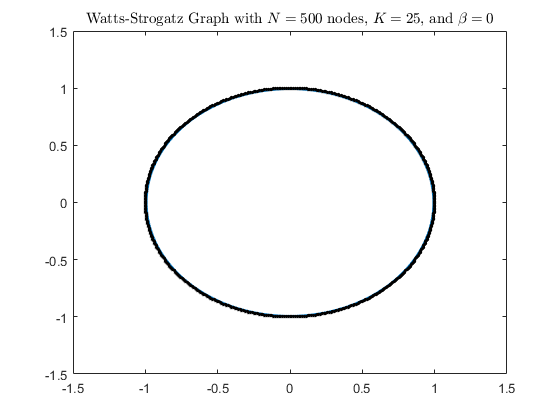
\includegraphics[height=6cm]{images/37.jpg}
            \end{figure}
            \par
            通过提高$\beta = 0.5$来增加图中的随机性
            \begin{lstlisting}[language=Matlab]
            h3 = WattsStrogatz(500, 25, 0.5);
            plot(h3, 'NodeColor', 'k', 'EdgeAlpha', 0.1);
            title('Watts-Strogatz Graph with $N = 500$ nodes, $K = 25$, and $\beta = 0.50$', ...
                'Interpreter','latex')
             \end{lstlisting}
            \begin{figure}[H]
            \centering
            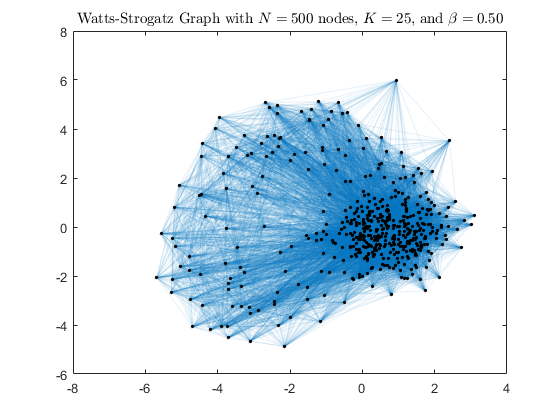
\includegraphics[height=6cm]{images/38.jpg}
            \end{figure}
            我们通过增加$\beta$,生成一个完全随机图,使其达到最大值1.0。
            \begin{lstlisting}[language=Matlab]
            h4 = WattsStrogatz(500,25,1);
            plot(h4,'NodeColor','k','EdgeAlpha',0.1);
            title('Watts-Strogatz Graph with $N = 500$ nodes, $K = 25$, and $\beta = 1$', ...
            'Interpreter','latex')
             \end{lstlisting}
            \begin{figure}[H]
            \centering
            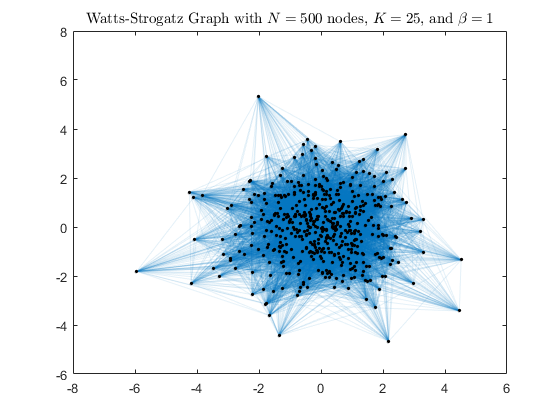
\includegraphics[height=6cm]{images/39.jpg}
            \end{figure}
            \textbf{3、网络特征 - 度分布}
            \par
            节点的度分布在不同的Watts-Strogatz图是不同。当$\beta$是0时,每个节点都有相同的度$2K$,所以度是一个狄拉克$\delta$函数分布$\delta(x-2K)$。然而,随着$\beta$增加,程度分布在发生变化。下面的图显示了度分布的变化。
            \begin{lstlisting}[language=Matlab]
            histogram(degree(h2),'BinMethod','integers','FaceAlpha',0.9);
            hold on
            histogram(degree(h3),'BinMethod','integers','FaceAlpha',0.9);
            histogram(degree(h4),'BinMethod','integers','FaceAlpha',0.8);
            hold off
            title('Node degree distributions for Watts-Strogatz Model Graphs')
            xlabel('Degree of node')
            ylabel('Number of nodes')
            legend('\beta = 1.0','\beta = 0.50','\beta = 0.15','Location','NorthWest')
             \end{lstlisting}
            \begin{figure}[H]
            \centering
            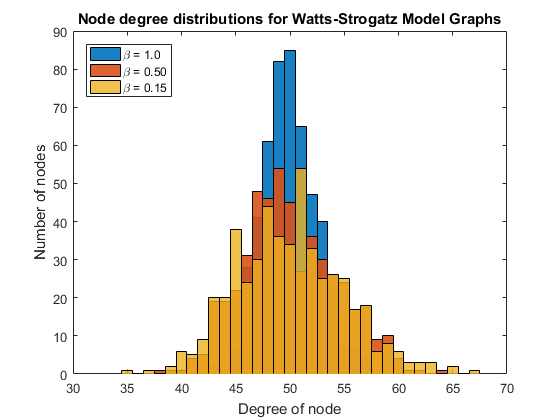
\includegraphics[height=6cm]{images/40.jpg}
            \end{figure}
            \textbf{4、网络特征 - 中心的形成}
            \par
            因为Watts-Strogatz图聚类系数高,所以节点倾向于形成小团体,或小组密切联系的节点。随着$\beta$增加,它的最大值也在增加,你会看到越来越大量的枢纽节点,或节点的相对程度高。中心是一个常见的其他节点之间的连接和派系之间的图。中心的存在就是允许派系的形成,同时保留一个简短的平均路径长度。
            计算的平均路径长度和数量为每个$\beta$值的中心节点。在示例中,节点与中心节点度大于或等于55。 这些所有的节点的度增加$10\%$或更多比原环晶格。
            \begin{lstlisting}[language=Matlab]
            n = 55;
            d = [mean(mean(distances(h))), nnz(degree(h)>=n); ...
                 mean(mean(distances(h2))), nnz(degree(h2)>=n); ...
                 mean(mean(distances(h3))), nnz(degree(h3)>=n);
                 mean(mean(distances(h4))), nnz(degree(h4)>=n)];
            T = table([0 0.15 0.50 1]', d(:,1), d(:,2),...
                'VariableNames',{'Beta','AvgPathLength','NumberOfHubs'})
                 \end{lstlisting}
            \par
            作为$\beta$平均路径长度的增加,图很快就落在了它的极限值。这是由于形成高度连接的枢纽节点,成为更多$\beta$增加。画出 的Watts-Strogatz模型图,使每个节点的大小和颜色的程度成正比。这是一个有效的方法来可视化中心的形成。
            \begin{lstlisting}[language=Matlab]
            colormaphsv
            deg=degree(h2);
            nSizes=2*sqrt(deg-min(deg)+0。2);
            nColors=deg;
            plot(h2,'MarkerSize',nSizes,'NodeCData',nColors,'EdgeAlpha',0。1)
            title('Watts-StrogatzGraphwith$N=500$nodes,$K=25$,and$\beta=0。15$',。。。
            'Interpreter','latex')
            colorbar
             \end{lstlisting}
            \begin{figure}[H]
            \centering
            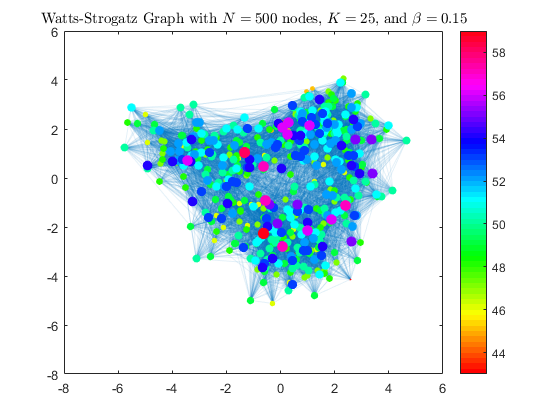
\includegraphics[height=6cm]{images/41.jpg}
            \end{figure}
            % \textcolor[rgb]{1.00,0.00,0.00}{实例3知乎爬虫}\\
            % \noindent Matlab图论算法及工具箱\\
            % \noindent 白纸上的例子这里我没有写上!!!!
    \subsection{金融时间序列结构fints}
        \par
        fints用于构建金融时间序列数据,可以用于单一时间序列分析,也可以用于多元时间序列分析。更多情况下,fints被用来进行股票数据分析,其基本结构如下表(\ref{tab:股票数据基本结构})所示
        \begin{table}[H]
        \centering
        \caption{股票数据基本结构}
        \label{tab:股票数据基本结构}
          \begin{tabular}{c|c|c}
            \hline
            Dates & Series1 & Series2\\
            \hline
            \vdots &\vdots & \vdots \\
            \vdots &\vdots & \vdots \\
        \end{tabular}
        \end{table}
        fints数据结构的构建方法(工厂函数法)为:
        \par
        tsobj = fints(dates, data, datanames, freq, desc)\\
        其中:dates表示日期,关于日期的形式(格式)及函数在后面介绍;data表示时间序列,可以是列向量也可以是矩阵;datanames表示时间序列名称,默认为series1$\dots$,可以用$\{'', ''\}$定义;freq表示频率指示器,允许的取值如下
        \begin{table}[H]
        \centering
        \label{tab:freq允许的取值有}
          \begin{tabular}{l|l}
            \hline
            Unkown & 0\\
            \hline
            Daily &1\\
            \hline
            Weekly & 2\\
            \hline
            monthly &3\\
            \hline
            Quarterly &4\\
            \hline
            Semiannually & 5\\
            \hline
            Annual & 6\\
            \hline
        \end{tabular}
        \end{table}
        \par
        desc表示时序的描述.character vector类.default=’’(默认为缺省)。对fints进行访问时,每行为一单元(个体),可以用dot index(.seriesname)形式访问某一序列,亦可两者结合使用A.series([3:6]),且操作(访问)后的子数据仍为fints数据格式。下面,我们将列举一些fints的常用函数,并给出一些简单的例子,如果读者想进一步学习该数据结构,可以访问下面的网址\footnote{http://cn.mathworks.com/help/finance/manage-financial-time-series.html\par
        http://cn.mathworks.com/help/finance/fints.html\par
        http://cn.mathworks.com/help/finance/data-transformation-and-frequency-conversion.html\par
        https://zhuanlan.zhihu.com/p/21454649?refer=matlab
        }。
        \subsubsection{fints数据结构的相关函数}
            \begin{longtable}{|l|l|}
            \hline
            \endfirsthead
            \multicolumn{2}{l}{(续表)}
            \endhead
            \hline
            \multicolumn{2}{c}{\itshape 接下页表格……}\\
            \endfoot
            \hline
            \endlastfoot
            \hline
            命令 & 说明 \\
            \hline
            fts2mat & {}\\\hline
            ascii2fts & {}\\\hline
            merge &取fts1, fts2两者时刻交集为索引\\\hline
            convertto(fts, ’daily’) &按daily采样,自动过滤节假日\\\hline
            todaily(fts)  & {}\\\hline
            resamplets(fts, step) &step为采样步长\\\hline
            boxcox  &Box-Cox变换\\\hline
            diff  & {}\\\hline
            fillts  & {}\\\hline
            filter & {} \\\hline
            leadts & {}\\\hline
            peravg  &计算一定周期内的均值\\\hline
            smoothts & {}\\\hline
            tsmovavg  &计算移动平均值,需要R2016a版本\\\hline
            chartfits & {}\\\hline
            ftstool & {}\\\hline
            ftsbound & {}\\\hline
            horzcat & {}\\\hline
            vertcat & {}\\\hline
            corrcoef & Correlation coefficients\\\hline
            cov & Covariance matrix\\\hline
            isempty & True for empty financial time series objects\\\hline
            nancov & Covariance ignoring NaNs\\\hline
            nanmax & Maximum ignoring NaNs\\\hline
            nanmean & Mean ignoring NaNs\\\hline
            nanmedian & Median ignoring NaNs\\\hline
            nanmin & Minimum ignoring NaNs\\\hline
            nanstd & Standard deviation ignoring NaNs\\\hline
            nansum & Sum ignoring NaNs\\\hline
            nanvar & Variance ignoring NaNs\\\hline
            var & Variance\\\hline
            chfield & 改变数据系列的名字\\\hline
            eq(fts) & 多个金融时报系列对象平等\\\hline
            extfield & 数据提取\\\hline
            fetch & 金融时间序列的数据对象\\\hline
            fieldnames & 获得字段的名称\\\hline
            freqnum & 特征向量频率指标转换为数字 频率指标\\\hline
            freqstr & 数字频率指标转化为特征向量 表示\\\hline
            ftsbound& 开始和结束日期\\\hline
            ftsinfo  & 金融时间序列对象信息\\\hline
            ftsuniq & 确定的独特性\\\hline
            getfield & 内容的特定字段\\\hline
            getnameidx  &在名单上找到的名字\\\hline
            iscompatible & 结构上的平等\\\hline
            isequal & 多个对象平等\\\hline
            isfield & 检查是否特征向量是字段名\\\hline
            issorted & 检查日期和时间是否单调递增\\\hline
            rmfield &  删除数据系列\\\hline
            setfield & 设置特定字段的内容\\\hline
            sortfts  & 类金融时间序列\\\hline
            \end{longtable}
            \noindent
            注:1、平滑方法有linear、exponential、accussion等方法;
            \par
            2、peravg的返回值也是一个结构体;
            \par
            3、在FINTS中,用 “::”来指定一段时间;
            \par
            4、索引index 的只能是行数。
        \subsubsection{ 示例}
            \par
            此文档是fts数据类的一个简单示例。fts数据类来自matlab金融工具箱,主要用来进行股票等金融数据分析。我们直接利用matlab自带的数据给出示例(fts的创建、索引和方法等),读者可以到下面的网址 了解详细的内容。当然,你也可以在命令窗口运行:
            \begin{lstlisting}[language= Matlab]
            openExample('finance/UsingTimeSeriestoPredictEquityReturnExample')
            \end{lstlisting}
            命令来查看这个示例。数据存放在 $predict\_ret\_data.mat$这个MAT数据文件,这个MAT文件包含6个变量(矢量):1. corresponding to the closing stock prices, sdates;2. Closing stock prices, sdata;3. Dividend dates, divdates;4. Dividend paid, divdata;5. Dates corresponding to the metric(度量标准) data, expdates;6. Metric data, expdata。\\
            1、加载数据
                \begin{lstlisting}[language=Matlab]
                clc, clear
                load predict_ret_data.mat
                whos
                \end{lstlisting}
            2、创建金融时间序列对象
                \begin{lstlisting}[language=Matlab]
                t0 = fints(sdates, sdata, {'Close'}, 'd', 'Inc');%股票收盘价\stock closing prices
                d0 = fints(divdates, divdata, {'Dividends'}, 'u', 'Inc');%股息支付\dividend payments
                x0 = fints(expdates, expdata, {'Metric'}, 'w', 'Index');%explanatory data
                srs2 = t0.Close(1:5)%点索引指示变量Close,(1:5)序号索引指示前5行
                srs2_vec = fts2mat(t0.Close(1:5))
                t0.Close('05-Jan-1999')%时间索引
                t0({'05/11/99', '05/21/99', '05/31/99'})
                t0.Close({'05/11/99', '05/21/99', '05/31/99'})
                t0('05/11/99::05/15/99')%::表示from to
                nfts = t0.Close('05/11/99::05/20/99');
                \end{lstlisting}
            3、fts数据类型的基本操作
                \begin{lstlisting}[language=Matlab]
                %% 创建收盘价调整series
            dadj1 = d0;
            dadj1.dates = dadj1.dates-1;
            dadj2 = d0;
            dadj2.Dividends = 0;
            dadj2 = fillts(dadj2,'linear','12/31/98');
            dadj2('12/31/98') = 0;
            dadj3 = [dadj1; dadj2];
            dadj3 = fillts(dadj3, 'linear', t0.dates);
            %% 现货价格。
            t0.Spot = t0.Close - fts2mat(dadj3(datestr(t0.dates)));
            %% 创建返回系列。
            tret = (t0.Spot - lagts(t0.Spot, 1)) ./ lagts(t0.Spot, 1);
            tret = chfield(tret, 'Spot', 'Return');
            %%  Regress return series against metric data.
            x1 = todaily(x0);
            x1.Const = 1;
            dcommon = intersect(tret.dates, x1.dates);
            regts0  = [tret(datestr(dcommon)), x1(datestr(dcommon))];
            finite_regts0 = find(all(isfinite( fts2mat(regts0)), 2));
            regts1        = regts0( finite_regts0 );
            DataMatrix = fts2mat(regts1);
            XCoeff     = DataMatrix(:, 2:3) \ DataMatrix(:, 1);
            RetPred = DataMatrix(:,2:3) * XCoeff;
            tret.PredReturn(datestr(regts1.dates)) = RetPred;
                \end{lstlisting}
            4、绘制、计算结果
                \begin{lstlisting}[language=Matlab]
                    subplot(2, 1, 1);
                    plot(t0);
                    title('Spot and Closing Prices of Stock');
                    subplot(2, 1, 2);
                    plot(tret);
                    title('Actual and Predicted Return of Stock');
                    %% 计算股息率。
                    datestr(d0.dates, 2)
                    t1 = fillts(t0,'nearest',d0.dates);
                    t1.freq = 'd';
                    tdr = d0./fts2mat(t1.Close(datestr(d0.dates)))   % Calculate the dividend rate
                \end{lstlisting}
        \subsubsection{引入 - Quantmod(R package)}
            \par
            在R当中可用于金融数据实证研究的R包数量很多,目前在CRAN中的这些R包大多数侧重比较学术化的金融数据的计量研究\footnote{http://cran.r-project.org/web/views/Finance.html},比如著名的Rmetrics系列。quantmod\footnote{http://www.quantmod.com}是R用于金融建模的扩展包,使用R做金融大数据处理几乎必用此扩展软件包,其主要功能有:从多个数据源获取历史数据、绘制金融数据图表、在金融数据图表中添加技术指标、计算不同时间尺度的收益率、金融时间序列分析、金融模型拟合与计算等等。quantmod可以从下面的来源加载数据:
            \begin{itemize}
              \item Yahoo! Finance (OHLC data)
              \item Federal Reserve Bank of St. Louis FRED® (11,000 economic series)
              \item Google Finance (OHLC data)
              \item Oanda, The Currency Site (FX and Metals)
              \item MySQL databases (Your local data)
              \item R binary(二进制的) formats (.RData and .rda)
              \item Comma Separated Value files (.csv)
              \item More to come including (RODBC,economagic,Rbloomberg,...)
            \end{itemize}
            \par
            下面,我们将简单介绍quantmod的一些函数并给出一个简单的示例,如果你想进一步了解quantmod,可以参考以下网址\footnote{http://www.quantmod.com/examples/intro/
            http://www.quantmod.com/examples/data/
            http://www.quantmod.com/examples/charting/
            }。\\
            示例:
                \begin{lstlisting}[language = R]
                  install.package(“quantmod”)
                  library(quantmod)   # Load the package
                  getSymbols("AAPL")  # Download daily prices of Apple stock from Yahoo
                  chartSeries(AAPL, theme="white")  # Plot the daily price and volume
                  chartSeries(AAPL) # Not shown giving the same plot with black background.
                  getSymbols("AAPL",from="2005-01-02", to="2010-12-31")
                  AAPL <- Delt(Cl(get("AAPL", env = new.environment)))
                  length(AAPL[which(AAPL > 0.02), ])       #查看AAPL涨跌幅超过2%的情况
                  plot(AAPL[which(AAPL > 0.02), ])         #画出AAPL涨跌幅超过2%的情况
                \end{lstlisting}
            \textbf{一、ETL类函数}
            \par
            getSymbols("AAPL", src = "yahoo", from = "2005-01-02", to = "2010-12-31")
            其中,src可以设置为“yahoo”、”google”、”FRED”、”Oanda”等。更为详细的ETL函数说明可以参考表(\ref{tab:ETL函数说明})
            \begin{table}[H]
            \centering
            \caption{ETL函数说明}
            \label{tab:ETL函数说明}
            \newcolumntype{Y}{>{\centering\arraybackslash}X}
                \begin{tabularx}{\textwidth}{lXlX}
                \toprule
            函数 & 作用&函数 & 作用\\\midrule
            getSymbols()   &从多种信息源里获得信息& getSymbols.csv()  &从csv文件中读入数据  \\
            getDividends () &获取上市公司的股息数据& getSymbols.FRED() &从FRED中获取数据\\
            getFinancials () &获取上市公司的财务报表& getSymbols.Google() &从Google中获取数据\\
            getFX ()   &返获取汇率数据& getSymbols.MySQL()   &从MySQL中获取数据\\
            getMetals ()   &获取重金属交易数据 & getSymbols.oanda()  &从onada中获取数据\\
            getSplits ()  &获取上市公司的拆股数据 & getSymbols.rda()  &从R的二进制文件中获取数据\\
            getOptionChain () &获取期权交易数据& getSymbols.SQLite()   &从SQLite 数据库中获取数据\\
            getQuote () &获取即时的网络报价& getSymbols.yahoo()   &从雅虎网中获取数据\\
                \bottomrule
            \end{tabularx}
            \end{table}
            补充:提取某种数据类型(例如:开盘价,最高价等),有下列函数
            \begin{lstlisting}[language = R]
                  Op() #Open price 开盘价
                  Hi() #High price 最高价
                  Lo() #Low price 最低价
                  Cl() #Close price 收盘价
                  Vo() #volume 交易量
                  Ad() #Adjusted price 调整价格
                  HLC()
                  OHLC() #开盘价、最高价、最低价和收盘价
            \end{lstlisting}
              % \begin{table}[H]
              %     \centering
              %   \begin{tabular}{l|l}
              %     \toprule
              %     函数 & 说明\\
              %     \midrule

              %     \bottomrule
              %   \end{tabular}
              % \end{table}
            \noindent \textbf{二、展示类函数}
                \begin{lstlisting}[language=R]
            barchart                                                  #条形图
            candlechart(AAPL, multi.col = ’true’, theme = "white")    #蜡烛图
            linechart()                                               #线图
            chartSeries(to.weekly(AAPL), dn.col = "green", up.col = "red")
            addADX()
            addATR()
            addBBands()
            addCCI()
            addCMF()
                \end{lstlisting}
            \textbf{三、分析类函数}\\
            1、is族函数,判断某数据是否是某类型的数据,例如:
                \begin{lstlisting}[language=Matlab]
            is.OHLC()
            is.OHLCV()
            is.BBO()
            is.TBBO()
            is.HLC()
                \end{lstlisting}
            2、has族函数,检查数据里面是否包含某类型的数据,例如:
                \begin{lstlisting}[language=R]
            has.OHLC()
            has.HLC()
            has.OHLCV()
            has.Op()
            has.Hi()
            has.Lo()
            has.Cl()
            has.Vo()
            has.Ad()
            has.Bid()
            has.Price()
            has.Qty()
            has.Trade()
                \end{lstlisting}
            \textbf{四、计算类函数}
              \begin{table}[H]
                  \centering
                \begin{tabular}{l|l}
                  \toprule
                  函数 & 说明\\
                  \midrule
            to.weekly() & 将OHLC数据转化为周数据\\
            to.monthly() & 将OHLC数据转化为月数据\\
            Delt() & 计算变化率\\
            Lag() & 求滞后k期\\
            Next() & 求k个后\\
            first() & 求前k个\\
            last() & 求后k个\\
            findPeaks() &  找出峰值\\
            findValleys() & 找出谷值\\
            seriesIncr() & 差分后大于限值的点\\
            seriesDecr() & 差分后小于限值的点\\
            endpoints() & 寻找节点\\
            periodicity() & 返回数据的日期范围\\
                  \bottomrule
                \end{tabular}
              \end{table}
    \subsection{cell和struct数据结构}
        \subsubsection{cell 元胞数组}
            \par
            元胞数组和结构体数组是两种比较常见的数据类型,在一般的书籍中都有详细介绍,这里我们仅简单介绍一下两个数组的构建方法以及可用的命令(函数)。对于元胞数组而言,可以将其视为储物柜,每个储物柜(cell的单元)可以存放不同类型的事物。但是,在进行单元提取时,我们应该注意是使用()还是$\{\}$来进行索引。
            cell构建方法:直接赋值和工厂函数
            \begin{lstlisting}[language = Matlab]
            cellname{i, j} = {value}
            cellname = cell(m, n)
            \end{lstlisting}
            \par
            其可用函数如下表
              \begin{table}[H]
                  \centering
                \begin{tabular}{llll}
                  \toprule
                  命令 & 说明&命令 & 说明\\
                  \midrule
            cellstr& 字符型数组&mat2cell & 将数值矩阵转变成为元胞数组\\
            iscell & 判断输入是否为元胞数组&num2cell & 将数值数组转变成为元胞数组\\
            cellfun &为元胞数组的每个元胞执行指定的函数&cell2struct & 将元胞数组转变成为结构\\
            celldisp & 显示所有元胞的内容&struct2cell & 将结构转变为元胞数组\\
            cellplot & 利用图形方式显示元胞数组&deal & 将输入参数赋值给输出\\
            cell2mat & 将元胞数组转变成为普通的矩阵&length & {}\\
                  \bottomrule
                \end{tabular}
              \end{table}
        \subsubsection{struct结构体数组}
            struct构建方法:直接赋值和工厂函数(这里注意两个概念:域名fieldname、域值fieldvalue)
            \begin{lstlisting}[language = Matlab]
            struct.name(i, j).fieldname(m, n) = field value;
            struct.name = struct(‘fieldname’, {fieldvalue}, …);
            \end{lstlisting}
            \par
            可用函数如下表所示
              \begin{table}[H]
                  \centering
                \begin{tabular}{llll}
                  \toprule
                  命令 & 说明&命令 & 说明\\
                  \midrule
            isstruct & 确定输入是否为结构体数组&arrayfun  &  将函数应用于每个数组元素\\
            fieldnames & 结构体的字段名称或对象的公共字段&structfun  & 对标量结构体的每个字段应用函数\\
            getfield & 结构体数组字段&table2struct & 将表转换为结构体数组\\
            isfield &确定输入是否为结构体数组字段&struct2table & 将结构体数组转换为表\\
            orderfields  & 结构体数组的顺序字段&cell2struct &将元胞数组转换为结构体数组\\
            rmfield  & 删除结构体中的字段&struct2cell &将结构体转换为元胞数组\\
            setfield  &  向结构体数组字段分配值&size & {}\\
            cat &提取结构体数组值并按顺序排列&length & {} \\
                  \bottomrule
                \end{tabular}
              \end{table}
            示例:
            \begin{lstlisting}[language=Matlab]
            [Y1, Y2, ...] = deal(structname(i, j).fieldname1, structname(i, j).fieldname2, ...)
            Y1 = structname(i, j).fieldname1
            Y2 = structname(i, j).fieldname2
            setfield(structname, ’fieldname’, fieldvalue)
            setfield(structname, {i,j}, ’fieldname’, {m, n}, fieldvalue)
            struct(i, j).fieldname(m, n).fieldname = fieldname
            \end{lstlisting}
    \subsection{分类数组Categorical Arrays}
        \par
        Categorical数组用于处理分类数据(就是市场调查中常见的数据类型)。对于分类数据,我们经常绘制一些变量的频数(频率)图、比例图(饼图)等等,而对于这种数据的分析,我们经常用到决策树分类、对应分析以及卡方检验等等。如果读者想进一步了解这种数据类型,可以参考下面的网址\footnote{http://cn.mathworks.com/help/matlab/categorical-arrays.html}。
        \subsubsection{函数说明}
            \begin{table}[H]
            \centering
            \newcolumntype{Y}{>{\centering\arraybackslash}X}
                \begin{tabularx}{\textwidth}{lXlX}
                \toprule
             命令& 说明& 命令& 说明\\\midrule
            categorical & 创建分类数组 & removecats & 删除类别分类数组\\
            iscategorical  & 确定输入是否分类数组&renamecats & 重命名类别分类数组中\\
            categories & 类别的分类数组&reordercats & 重新排序类别分类数组中\\
            iscategory & 测试类别分类数组&setcats & 设置类别分类数组\\
            isordinal & 确定输入顺序分类数组&summary & 打印的总结表或分类数组\\
            isprotected&确定类别的分类数组 受保护的&countcats & 按类别分类数组元素的计数\\
            addcats & 添加类别分类数组&isundefined & 发现未定义的元素分类数组\\
            mergecats & 合并类别分类数组&{}&{}\\
                \bottomrule
            \end{tabularx}
            \end{table}
        \subsubsection{示例}
            此文档是Categorical Arrays数据类的一个简单示例。Categorical数据类型是用来处理分类数据的,这种数据(变量)在市场调查中经常出现,变量的取值不是数值类型的,而是分类的(例如:男、女)。下面,我们来简单示例Categorical数据类型的创建、索引和方法,我们仍然采用MATLAB自带的数据parents,这个数据集(patients.mat文件)中包含的变量在table类中进行了介绍,这里不再继续介绍。\\
            1、创建categorical类型
                \begin{lstlisting}[language=Matlab]
            clc, clear
            load patients
            whos
            T = table(Age,Gender,Height,Weight,...
                SelfAssessedHealthStatus,Location,...
                'RowNames',LastName);%创建table变量
            T.Gender = categorical(T.Gender);%创建categorical变量
            T.Location = categorical(T.Location);
            class(T.Location)
            categories(T.Location)%查看变量的分类
            C = T.Gender.*T.Location;%categorical变量合并
            C(1:5)
            categories(C)
            T.SelfAssessedHealthStatus = categorical(T.SelfAssessedHealthStatus,...
                {'Poor','Fair','Good','Excellent'},'Ordinal',true);
            rows = T.Location=='County General Hospital' & T.Gender=='Female';
            vars = {'Age','Height','Weight'};
            T1 = T(rows, vars);
                \end{lstlisting}
            2、绘制结果
                \begin{lstlisting}[language=Matlab]
            figure
            histogram(T.Location(T.SelfAssessedHealthStatus <= 'Fair'))
            title('Location of Patients in Fair or Poor Health')
            figure
            pie(T.SelfAssessedHealthStatus);
            title('Self Assessed Health Status From 100 Patients')
            figure
            A = countcats(T.SelfAssessedHealthStatus);
            C = categories(T.SelfAssessedHealthStatus);
            pareto(A, C);
            title('Self Assessed Health Status From 100 Patients')
            X1 = Weight(T.Gender=='Female');
            Y1 = Height(T.Gender=='Female');
            X2 = Weight(T.Gender=='Male');
            Y2 = Height(T.Gender=='Male');
            figure
            h1 = scatter(X1,Y1,'o');
            hold on
            h2 = scatter(X2,Y2,'x');
            xlabel('Weight (lbs)')
            ylabel('Height (in)')
            title('Height vs. Weight')
                \end{lstlisting}
    \subsection{字符串str}
        \subsubsection{字符串操作函数}
            \begin{longtable}{|l|l|}
            \hline
            \endfirsthead
            \multicolumn{2}{l}{(续表)}
            \endhead
            \hline
            \multicolumn{2}{c}{\itshape 接下页表格……}\\
            \endfoot
            \hline
            \endlastfoot
            命令 & 说明 \\
            \hline
            \multicolumn{2}{|c|}{检测字符类}\\
            \hline
            isstr &检测是否为字符串\\
            ischar & 检测字符串是否为字符数组\\
            isletter & 检测字符串中的英文字母\\
            isspace &检测字符串中每个字符是否属于格式字符(空格,回车等)\\
            isstrprop &检测字符串中符合特定范畴的字符\\
            isequal &可用来比较两个字符数组是否相同\\
            \hline
            \multicolumn{2}{|c|}{元胞数组类}\\
            \hline
            cellstr& 用于元胞数组元素为不定长字符串\\
            char & 转换元胞数组到字符数组,转换ASCII码到字符\\
            iscellstr &判断是否为元胞数组\\
            sort & 数组元素排序\\
            intersect& 数组交集,升序排列输出\\
            ismember & 判断是否为集合中的元素\\
            setdiff &数组差集,升序排列输出\\
            setxor & 数组异或,即不属于数组交集的元素,升序排列输出\\
            union &数组并集,升序排列输出\\
            unique & 查找数组中独特的元素序列\\
            \hline
            \multicolumn{2}{|c|}{字符操作类}\\
            \hline
            strcat & 字符串连接\\
            strvcat &字符串垂直连接\\
            strcmp & 判断字符串是否相等\\
            strncmp &判断两个字符串的前n个字符是否相等\\
            strcmpi &判断字符串是否相等,忽略大小写\\
            strncmpi & 判断两个字符串的前n个字符是否相等,忽略大小写\\
            strrep(s,s1,s2) &替换字符串s中的s1为s2\\
            strfind(s,s1) &查找字符串s中串s1的位置\\
            findstr(s1,s2) & 查找短字符串在长字符串中的位置\\
            strtok(s,char) & 对字符串s中首个char前后分割\\
            strmatch(patten,str)&  检查patten是否和str最左侧部分一致\\
            regexp & 正则表达式\\
            regexpi &匹配正则表达式(不分大小写)\\
            regexprep &使用正则表达式替换文本\\
            regexptranslate &将文本转换为正则表达式\\
            lower &转换字符串中的字母为小写\\
            upper &转换字符串中的字母为小写\\
            strjoin &加入文本数组\\
            strsplit & 分割字符串指定的分隔符\\
            strjust &为字符串或字符数组\\
            strtrim &删除前导和尾随空白字符串数组 或字符数组\\
            \hline
            \multicolumn{2}{|c|}{数据转换类}\\
            \hline
            {}&这一部分前面好像有\\
            \hline
            \multicolumn{2}{|c|}{空格处理类}\\
            \hline
            blanks & 创建空格字符串\\
            deblank &去除字符串尾部空格\\
            strjust &字符串对齐 \\
            strtrim &去除字符串头尾空格,制表,回车符\\
            \hline
            \multicolumn{2}{|c|}{格式字符类}\\
            \hline
            eval&  eval可以用来执行用字符串表示的表达式\\
            sprintf& 按格式写数据到字符串\\
            fprintf& 按格式写数据到文件\\
            sscanf & 按格式从字符串中读取数\\
            texlabel & 把字符串转换成tex软件的格式\\
            bitand & {}\\
            bitor& {}\\
            bitxor&  {}\\
            bitget & 用来获取二进制的数位\\
            bitset & 设定某个二进制数位的值\\
            bin2hex &{}\\
            \hline
            \end{longtable}
        \subsubsection{函数示例及详细说明}
            \par
            待补充。。。
    \subsection{字符串数组str array}
        \par
        这个数据类型有别于字符数组char和cellstr。字符串str是str array、char和cellstr的基础,就像元素和集合的关系一样。为了对它们进行区别,你可以运行下面的命令进行研究,不过,要创建str array你需要R2016b或者更高版本。
                \begin{lstlisting}[language=Matlab]
            clc, clear
            str1 = 'i love matlab' %这是一个字符串
            str2 = ['I     '; 'love  '; 'matlab'] %这是字符数组,每一行必须具有相同的列数,不够以空格填补
            str3 = char('i', 'love', 'matlab') %这是字符数组,char函数会自动补充空格
            str4 = {'i','love','matlab'} %在cellstr中,每个单元可以是完全不同的内容,所以,不需要补充空格。
            str5 = string({'i','love','matlab'})%创建字符串向量
            whos
                \end{lstlisting}
        \subsubsection{可用函数}
            \begin{longtable}{|l|l|}
            \hline
            \endfirsthead
            \multicolumn{2}{l}{(续表)}
            \endhead
            \hline
            \multicolumn{2}{c}{\itshape 接下页表格……}\\
            \endfoot
            \hline
            \endlastfoot
            \hline
            命令 & 说明 \\
            \hline
            string & 创建字符串数组\\\hline
            strings  & 创建字符串数组(with no characters)\\\hline
            join & 把字符串,或合并两个表或时间表 行使用关键变量\\\hline
            newline  & 创建换行符\\\hline
            compose  & 将数据转换成格式化的字符串数组\\\hline
            sprintf  & 格式的数据转换成字符串\\\hline
            strcat & 横向连接字符串\\\hline
            isstring & 判断输入的字符串数组\\\hline
            strlength  & 字符串在字符串数组的长度\\\hline
            symvar & 确定符号变量表达式\\\hline
            contains & 确定模式的字符串\\\hline
            count  & 计数模式的字符串\\\hline
            endsWith & 确定字符串结尾的模式\\\hline
            startsWith & 确定字符串开始的模式\\\hline
            replace  & 查找和替换字符串中的子字符串数组\\\hline
            replaceBetween & 替换子字符串被马克的指标 他们开始和结束\\\hline
            split &  分割字符串在字符串数组,或把日历时间 数字和时间单位\\\hline
            splitlines & 在换行字符分割字符串\\\hline
            erase &  删除字符串中的子字符串\\\hline
            eraseBetween & 马克开始删除子字符串之间的指标 和结束的子字符串\\\hline
            extractAfter & 提取子字符串在指定的位置\\\hline
            extractBefore &  提取子字符串在指定位置\\\hline
            extractBetween & 马克开始提取子字符串之间的指标 和结束的子字符串\\\hline
            insertAfter &  后插入字符串指定的子串\\\hline
            insertBefore & 插入字符串之前指定的子串\\\hline
            pad  & 领先或落后于字符添加到字符串\\\hline
            strip &  删除前导和尾随字符的字符串\\\hline
            reverse &  相反的顺序的字符在字符串\\\hline
            strtrim& 删除前导和尾随空白字符串数组或字符数组\\\hline
            deblank &{}\\\hline
            lower &{}\\\hline
            upper&{} \\\hline
            strjust &{}\\\hline
            \end{longtable}
            示例
                \begin{lstlisting}[language=Matlab]
            openExample('matlab/RepresentTextWithCharacterAndStringArraysExample')
            openExample('matlab/AnalyzeTextDataExample')
            openExample('matlab/TestForEmptyStringsAndMissingValuesExample')
            openExample('matlab/SearchAndReplaceInStringAndCharacterArraysExample')
            openExample('matlab/CompareSortAndCharacterizeTextExample')
                \end{lstlisting}
            正则表达式参考\footnote{http://cn.mathworks.com/help/matlab/matlab\_prog/regular-expressions.html}
    \subsection{timeseries}
        \subsubsection{可用函数}
            \par
            timeseries结构可用的函数如下表所示\footnote{http://cn.mathworks.com/help/matlab/time-series-objects.html}
            \begin{longtable}{|l|l|}
            \hline
            \endfirsthead
            \multicolumn{2}{l}{(续表)}
            \endhead
            \hline
            \multicolumn{2}{c}{\itshape 接下页表格……}\\
            \endfoot
            \hline
            \endlastfoot
            \hline
            命令 & 说明 \\
            \hline
            append  &连接时间序列对象在时间维度\\
            get &  查询timeseries对象属性值\\
            getdatasamplesize  & 在timeseries数据样本对象的大小\\
            getqualitydesc & 数据质量描述\\
            getsamples & 时间序列样本使用下标索引的子集 数组\\
            plot & 情节时间序列\\
            set &  timeseries对象的设置属性\\
            tsdata.event & timeseries对象的构造事件对象\\
            timeseries & 创建timeseries对象\\
            \hline
            \multicolumn{2}{|c|}{添加或删除数据,操纵timeseries对象}\\
            \hline
            addsample &  添加数据样本timeseries对象\\
            delsample  & 将样品从timeseries对象\\
            detrend  & 减去均值或最佳线和nan从timeseries对象\\
            filter & 时间序列的频率的内容\\
            getabstime  &提取的时间字符串时间矢量单元阵列\\
            getdatasamples & 返回的时间序列样本子集用下标 索引数组\\
            getinterpmethod  & 插值方法timeseries对象\\
            getsampleusingtime  &样本中提取数据到新的timeseries对象\\
            idealfilter  & 理想(因果)滤波器应用于timeseries对象\\
            resample  &选择或插入timeseries数据 使用新的时间向量\\
            setabstime & timeseries的对象设置为日期 字符串\\
            setinterpmethod  & 设置默认为timeseries对象插值法\\
            setuniformtime & 修改统一时间timeseries对象的向量\\
            synchronize  & 同步和两个timeseries对象重新取样使用常见的时间向量\\
            \hline
            \multicolumn{2}{|c|}{添加或删除事件,创建新的timeseries对象 基于事件数据}\\
            \hline
            addevent & 添加事件timeseries对象\\
            delevent & 删除tsdata,事件对象从timeseries对象\\
            gettsafteratevent &新的timeseries对象和样本 在或在事件发生\\
            gettsafterevent &新的timeseries对象和样本 事件发生后\\
            gettsatevent & 新的timeseries对象和样本 发生的事件\\
            gettsbeforeatevent & 新的timeseries对象和样本 在事件发生之前或\\
            gettsbeforeevent & 新的timeseries对象和样本 之前发生的事件\\
            gettsbetweenevents & 新的timeseries对象和样本 发生事件之间\\
            \hline
            \multicolumn{2}{|c|}{时间序列集合}\\
            \hline
            get(tscollection)  & 查询tscollection对象属性 值\\
            isempty(tscollection)  & 确定tscollection对象 是空的\\
            length (tscollection)  & 向量的时间长度\\
            plot & 情节时间序列\\
            set(tscollection)  & tscollection对象的设置属性\\
            size(tscollection) & tscollection对象的大小\\
            tscollection & 创建tscollection对象\\
            addsampletocollection  & 添加示例tscollection对象\\
            addts  & timeseries对象添加到tscollection对象\\
            delsamplefromcollection &  将样品从tscollection对象\\
            getabstime(tscollection) & 提取的时间字符串时间矢量单元阵列\\
            getsampleusingtime(tscollection) & 样本中提取数据到新的tscollection对象\\
            gettimeseriesnames & 单元阵列timeseries对象的名称 在tscollection对象\\
            horzcat(tscollection) &  水平tscollection对象的连接\\
            removets & 删除从tscollection timeseries对象对象\\
            resample(tscollection) & 在tscollection使用选择或插入数据 新的时间向量\\
            setabstime(tscollection)  &设置tscollection对象 日期字符串\\
            settimeseriesnames & 改变tscollection timeseries对象的名称\\
            vertcat(tscollection)  & 垂直tscollection对象的连接\\
            \hline
            \end{longtable}
        \subsubsection{示例}
            \par
            此文档是time series数据类的一个简单示例。time seriesl数据类型用来处理时间序列。下面,我们来简单示例time seriesl数据类型的创建、索引和方法,我们仍然采用MATLAB自带的数据集count.mat,这是一个24-by-3 matrix(矩阵),有一个三岔路,每一列表示每小时从一路上经过的车辆数,共24小时。当然,如果你想详细了解这个示例,可以参考下面网址\footnote{http://cn.mathworks.com/help/matlab/data\_analysis/time\-series\-objects.html}。在下面的例子中,你将会学到ts时间序列对象和方法:创建时间序列对象;观察时间序列对象;修改时间序列的单位和插值方法;定义事件;创建时间序列集合对象;重采样时间序列集合对象;添加一个数据样本时间序列集合对象;删除和插值缺失的数据;移除一个时间序列的时间序列集合;显示时间矢量值日期字符串;策划时间序列集合成员。\\
            1、创建时间序列对象
                \begin{lstlisting}[language=Matlab]
            clc, clear
            load count.dat
            count1 = timeseries(count(:,1), 1:24,'name', 'intersection1');%创建ts
            count2 = timeseries(count(:,2), 1:24,'name', 'intersection2');
            count3 = timeseries(count(:,3), 1:24,'name', 'intersection3');
            get(count1)                    %查看属性/Query timeseries object property values
            count1.DataInfo
            count1.DataInfo.Units = 'cars';
            count1.DataInfo.Interpolation = tsdata.interpolation('zoh');
            count1.DataInfo
            count1.TimeInfo.Units = 'hours';
            count2.TimeInfo.Units = 'hours';
            count3.TimeInfo.Units = 'hours';
                \end{lstlisting}
            2、定义事件
                \begin{lstlisting}[language=Matlab]
            %Add two events to the data that mark the times of the AM commute and PM commute.
            e1 = tsdata.event('AMCommute',8);
            e1.Units = 'hours';            % Specify the units for time
            count1 = addevent(count1,e1);  % Add the event to count1
            count2 = addevent(count2,e1);
            count3 = addevent(count3,e1);
            %构造并添加第二个事件。 第二个事件发生在下午6点。
            e2 = tsdata.event('PMCommute',18);
            e2.Units = 'hours';            % Specify the  units for time
            count1 = addevent(count1,e2);  % Add the event to count1
            count2 = addevent(count2,e2);
            count3 = addevent(count3,e2);
            figure
            plot(count1)
            plot(count2)
            hold on
            plot(count3)
                \end{lstlisting}
            3、创建时间序列集合对象
                \begin{lstlisting}[language=Matlab]
            tsc = tscollection({count1 count2},'name', 'count_coll')
            tsc = addts(tsc, count3)
                \end{lstlisting}
            4、重采样时间序列集合对象
                \begin{lstlisting}[language=Matlab]
            tsc1 = resample(tsc,1:2:24)
            tsc1 = resample(tsc,1:0.5:24)
            hold off
            plot(tsc1.intersection1,'-xb','Displayname','Intersection 1')
            hold on
            plot(tsc1.intersection2,'-.xm','Displayname','Intersection 2')
            plot(tsc1.intersection3,':xr','Displayname','Intersection 3')
            legend('show','Location','NorthWest')
                \end{lstlisting}
            5、时间序列集合对象操作
                \begin{lstlisting}[language=Matlab]
            tsc1 = addsampletocollection(tsc1,'time',3.25,...
                   'intersection1',5);                        %添加一个数据样本到时间序列集合对象
            tsc1 = delsamplefromcollection(tsc1,'index',...
                   find(isnan(tsc1.intersection2.Data)));     %删除缺失的数据
            tsc1 = addsampletocollection(tsc1,'time',3.25,...
                   'intersection1',5);                        %插值缺失的数据
            tsc1 = resample(tsc1,tsc1.Time);
            tsc1 = removets(tsc1,'intersection3')             %移除一个时间序列
            tsc1.TimeInfo.Units = 'hours';
            tsc1.TimeInfo.StartDate = '25-DEC-2009 00:00:00';
            tsc1.intersection1.DataInfo.Units = 'car count';
            tsc1.intersection2.DataInfo.Units = 'car count';
            hold off
            plot(tsc1.intersection1);
            plot(tsc1.intersection1,'-xb','Displayname','Intersection 1')
            hold on
            plot(tsc1.intersection2,'-.xm','Displayname','Intersection 2')
            legend('show','Location','NorthWest')
            tsc1.TimeInfo.Units = 'hours';
            tsc1.TimeInfo.Format = 'HH:MM';
            hold off
            plot(tsc1.intersection1,'-xb','Displayname','Intersection 1')
            % Prevent overwriting plot, but remove axis labels and title.
            hold on
            plot(tsc1.intersection2,'-.xm','Displayname','Intersection 2')
            legend('show','Location','NorthWest')
            xlabel('Time (hours)')
            ylabel('car count')
            grid on
                \end{lstlisting}
    \subsection{time table}
        \subsubsection{可用函数}
            time table结构可用的函数如下\footnote{http://cn.mathworks.com/help/matlab/timetables.html}
            \begin{table}[H]
            \centering
            \newcolumntype{Y}{>{\centering\arraybackslash}X}
            \begin{tabularx}{\textwidth}{lXlX}
            \toprule
            命令& 说明&命令& 说明\\
            \midrule
            timetable & 从工作空间变量创建时间表&vartype  & 下标变量类型的表或时间表\\
            lag  & 节省时间数据的时间表&rmmissing  & 删除丢失的条目\\
            table2timetable  & 转换表的时间表&issorted  &判断数组进行排序\\
            array2timetable  & 将数组转换为时间表&sortrows & 行数组排序、表或时间表\\
            timetable2table  & 时间表转换为表&unique & 独特的数组中的值\\
            istimetable  & 确定输入时间表&withtol &  时间对时间表行加下标\\
            isregular  & 确定在时间表是否正常&timerange &  时间范围为时间表行加下标\\
            retime & 重新取样或聚合数据的时间表,并解决重复或不规则的次&{}&{}\\
            synchronize &  同步时间表常见时间向量,并重新取样或聚合数据从输入时间表&{}&{}\\
            \bottomrule
            \end{tabularx}
            \end{table}

            \subsubsection{示例}
            此文档是timetable数据类的一个简单示例。timetable是在R2016b中新加的数据类型,是ts和table的合并。下面,我们将简单介绍这种数据类型的构建、索引及方法,如果读者想要详细学习这种数据类型,你可以访问网址\footnote{http://cn.mathworks.com/help/matlab/timetables.html},当然,如果你已经拥有MATALB2016b版本或者更高版本,你可以在命令窗口输入下面命令进行学习
            \begin{lstlisting}[language = Matlab]
            openExample('matlab/CleanTimetableWithMissingDuplicateOrIrregularTimesExample')
            openExample('matlab/ResampleAndAggregateDataInTimetableExample')
            openExample('matlab/CombineTimetablesAndSynchronizeTheirDataExample')
            openExample('matlab/SubscriptIntoTimesOfTimetableExample')
            \end{lstlisting}
            \par
            我们的示例仍然采用MATLAB自带的数据,我们采用indoors.csv和outdoors.mat两个数据集进行示例。\\
            1、创建timetable
                \begin{lstlisting}[language=Matlab]
            indoors = readtable(fullfile(matlabroot,'examples','matlab','indoors.csv'));
            indoors = table2timetable(indoors);%数据类型转换
            load(fullfile(matlabroot,'examples','matlab','outdoors'));
            TF = isregular(outdoors)
            dt = unique(diff(outdoors.Time))
            TT = retime(outdoors,'daily','mean');%'hourly','nearest'/'spline'
            tv = datetime(2015,11,15):hours(6):datetime(2015,11,18);
            tv.Format = 'dd-MMM-yyyy HH:mm:ss';
            TT = retime(outdoors,tv,'mean');
            TT(1:5,:)
                \end{lstlisting}
            2、索引
                \begin{lstlisting}[language=Matlab]
            tt = synchronize(indoors,outdoors);%合并
            %索引:http://cn.mathworks.com/help/matlab/matlab_prog/access-data-in-a-table.html
            summary(tt)
            tt.Time(1:5)%行列索引
            TR = timerange('2015-11-16','2015-12-31');
            TT2 = tt(TR,:);%时间索引
            TT2(end-4:end,:)
            tt({'2015-11-16 12:18:00','2015-12-31 21:15:00'},:)%时间索引
            rowTimes = {'2002-02-01','2003-02-07'};
            S = withtol(rowTimes,days(1));
            tt(S,:)
            S = vartype('numeric');
            TT2 = tt(:,S);
            A = TT2.Variables;
            A(1:5,:)
            A = tt(:,vartype('numeric')).Variables;
            A(1:5,:)
                \end{lstlisting}
            3、合并及绘图
                \begin{lstlisting}[language=Matlab]
            ttLinear = synchronize(indoors,outdoors,'union','linear');
            ttHourly = retime(ttLinear,tv,'mean');
            ttHourly = rmmissing(ttHourly);
            ttMeanVars = ttHourly.Variables./mean(ttHourly.Variables);
            plot(ttHourly.Time,ttMeanVars);
            legend(ttHourly.Properties.VariableNames,'Interpreter','none');
            xlabel('Time');
            ylabel('Normalized Weather Measurements');
            title('Mean Daily Weather Trends');
                \end{lstlisting}
    \subsection{向量化操作函数}
        \subsubsection{matlab向量化操作函数}
            \par
            wikipedia中的向量化操作的定义是:Vectorization is the more limited process of converting a computer program from a scalar implementation, which processes a single pair of operands at a time, to a vector implementation which processes one operation on multiple pairs of operands at once。向量化计算是一种特殊的并行计算的方式,相比于一般程序在同一时间只执行一个操作的方式,它可以在同一时间执行多次操作,通常是对不同的数据执行同样的一个或一批指令,或者说把指令应用于一个数组/向量\footnote{http://blog.itpub.net/7768182/viewspace-1121259/}。
            \par
            从MATLAB7.0开始,陆续增加了一些向量化函数,使用这些函数可以减少很多循环的使用,在保证代码运行效率的前提下,使代码更加简洁。需要说明的是,很多情况下,使用这些函数的运行效率并不比恰当使用循环快多少,使用它们主要是为了提高开发效率,使代码更加简洁。对于MATLAB向量化操作函数,我们将介绍以下九个函数:1.arrayfun;2.bsxfun;3.cellfun;4.structfun;5.spfun;6.splitapply;7.varfun;8.rowfun;9.accumarray。
            \begin{lstlisting}[language=Matlab]
            %% arrayfun
            %对array中的每个分量进行操作
            s(1).f1 = rand(3, 6);
            s(2).f1 = magic(12);
            s(3).f1 = ones(5, 10);
            counts = arrayfun(@(x) numel(x.f1), s) %计算个数
            [nrows, ncols] = arrayfun(@(x) size(x.f1), s) %把s中的每个分量作为x输入到@(x) size(x.f1)
            averages = arrayfun(@(x) mean(x.f1), s, 'UniformOutput', false)%因为输出字符向量是nonscalar,故设置 UniformOutput 为false。
            [J, I] = meshgrid(1:10);
            a = arrayfun(@(ii, jj) dblquad(@(u, v) sin(u)*sqrt(v), 0, ii, 0, jj), I, J);
            %% bsxfun Introduced in R2007a
            %对矩阵的列/行进行操作
            A = [1 2 10; 3 4 20; 9 6 15];
            C = bsxfun(@minus, A, mean(A));%A的每一列减去mean(A)
            D = bsxfun(@rdivide, C, std(A));%等价于(A - mean(A))./std(A)
            fun = @(a,b) a - exp(b);
            a = 1:7;
            b = pi*[0 1/4 1/3 1/2 2/3 3/4 1].';
            C = bsxfun(fun, a, b)
            %% cellfun
            %对cell中的每个元素进行操作
            C = {1:10, [2; 4; 6], []};
            [nrows, ncols] = cellfun(@size, C)
            days = {'Monday', 'Tuesday', 'Wednesday', 'Thursday', 'Friday'};
            abbrev = cellfun(@(x) x(1:3), days, 'UniformOutput', false)%因为输出字符向量是nonscalar,故设置 UniformOutput 为false。
            c1 = rand(5,1);  c2 = rand(10,1);  c3 = rand(15,1);
            d1 = rand(5,1);  d2 = rand(10,1);  d3 = rand(15,1);
            C = {c1, c2, c3};
            D = {d1, d2, d3};
            covCD = cellfun(@cov, C, D, 'UniformOutput', false)
            %% structfun
            %对struct中的每个元素进行操作,可以将每个元素看作x,带入@(x)
            s.f1 = 'Sunday';
            s.f2 = 'Monday';
            s.f3 = 'Tuesday';
            s.f4 = 'Wednesday';
            s.f5 = 'Thursday';
            s.f6 = 'Friday';
            s.f7 = 'Saturday';
            lengths = structfun(@numel, s)
            shortNames = structfun(@(x) ( x(1:3) ), s, 'UniformOutput', false)
            %% spfun
            %对稀疏矩阵的每个元素进行操作
            S = spdiags([1:4]', 0, 4, 4)
            f = spfun(@exp,S)
            %% splitapply 分组统计
            %将 X 划分为 G 指定的组,并向每个组应用函数 func。
            load patients
            G = findgroups(Gender);
            splitapply(@mean, Height, G)
            func = @(x,y) var(x-y);
            [G, smokers] = findgroups(Smoker);
            varBP = splitapply(func, Systolic, Diastolic, G)
            T = table(smokers, numPatients, varBP)
            mystats = @(x)[min(x) median(x) max(x)];
            G = findgroups(Gender,Smoker);
            Y = splitapply(mystats, Weight, G)
            DT = table(Height, Weight);
            GT = table(Gender, Smoker);
            meanBMIFcn = @(h,w)mean((w ./ (h.^2)) * 703);
            [G, results] = findgroups(GT);
            meanBMI = splitapply(meanBMIFcn, DT, G);
            results.meanBMI = meanBMI
            %% varfun Introduced in R2013b
            %向表 A 的每个变量应用函数 func,并在表 B 中返回值。
            A = table([0.71;-2.05;-0.35;-0.82;1.57], [0.23;0.12;-0.18;0.23;0.41])
            func = @(x) x.^2;
            B = varfun(func, A)%列操作
            A = table({'test2';'test1';'test2';'test3';'test1'},...
                [0.71;-2.05;-0.35;-0.82;1.57],[0.23;0.12;-0.18;0.23;0.41])
            func = @mean;
            B = varfun(func, A, 'GroupingVariables', 'Var1')
            %% rowfun Introduced in R2013b
            %将函数 func 应用于表 A 的每行并在表 B 中返回结果
            x = gallery('integerdata', 10, [5, 1], 2);
            y = gallery('integerdata', 10, [5, 1], 8);
            A = table(x, y)
            B = rowfun(@hypot, A, 'OutputVariableNames', 'z')
            g = gallery('integerdata',3,[15,1],1);
            x = gallery('uniformdata',[15,1],9);
            y = gallery('uniformdata',[15,1],2);
            A = table(g, x, y)
            func = @(x,y) mean(x-y);
            B = rowfun(func, A,...
                'GroupingVariable', 'g', ...
                'OutputVariableName', 'MeanDiff')
            %% accumarray
            %使用下标 subs 累积矢量 val 的元素来返回数组 A
            %生成一个100000×1的向量,找出哪些元素出现(各元素及其频数)
            c = unique(unidrnd(200000, 100000, 1));
            d = accumarry((unidrnd(200000, 100000, 1), 1, [200000, 1]);
            e = find(a)
            %在1000×1000的正方形区域随机生成100000个点,计算每个坐标点上生成点的个数
            P = unidrnd(1000, 100000, 2);
            a = accumarry((p, 1, [1000, 1000]);
            %1000人,身高分布在170-180,体重在110-200,年龄在20-50,计算身高体重相同的人的平均年龄
            Height = unidrnd(10, 1000,1) + 170;
            Weight = unidrnd(90, 1000, 1) + 110;
            Age = unidrnd(30, 1000, 1) + 20;
            m0 = accumarray([height, weight], age, [], @mean)
                \end{lstlisting}
        \subsubsection{引入 - Python和R中的向量化函数}
            \par
            \paragraph{R中的向量化函数}我们将简单介绍R中的向量化函数apply族函数以及plyr包和reshape包。
            \par
            (1)applay函数族包括了apply、sapply、lappy、tapply、mapply、sweep、aggregate, by等函数:\\
            1、apply:是处理矩阵/数组的,并逐行或逐列进行操作,内置(底层)为循环计算。\\
            Eg:apply(matrix, 1, mean) \#计算matrix每行(dim = 1)的均值\\
            \#注:对于矩阵还可以用colMeans、rowMeans、colSums,、rowSums做行列运算\\
            2、lapply:是处理向量/列表/其它对象,返回列表形式list。\\
            Eg:lapply(data.frame, FUN = function(x) list(median = median(x), sd = sd(x)))\#计算data.frame每列的中位数和标准差\\
            3、sapply:类似于lapply,但其返回为矩阵,等价于unlist(lapply())。\\
            Eg:sapply(data.frame, FUN = function(x) list(median = median(x), sd = sd(x))) \\
            4、tapply:是专门用来处理分组数据的(属性数据)。\\
            Eg:tapply(Sepal.Width, index = Species, FUN = mean) \#计算三种花瓣萼片宽度的均值\\
            5、aggreate:与tapply功能非常相似,其输出是更为友好的数据框格式。\\
            6、by和上面两个函数aggreate与tapply是出于一处的。\\
            7、replicate:将某个函数重复运行N次,常用来生成较复杂的随机数。\\
            8、vectorize:能将一个不能进行向量化运算的函数进行转化,使之具备向量化运算功能。\\
            9、maaply:是sapply的变形,将fun依次依次应用于每一个参数的第一个元素、第二个元素…\\
            Eg:mapply(fun = rep, times = 1:4, x = 4:10, moreArgs = Null, simplify = true,  rse.names = true)\\
            10、aaply:plyr包函数。\\
            Eg:a = matrix(1:21, nrow = 3, ncol = 7) b = aaply(a, .margins = 2, .fun = mean)\# 对a的每列求均值
            \par
            (2)plyr包\footnote{http://plyr.had.co.nz/09-user/}:
            \par
            plyr包的作者是RICE大学统计学的助理教授Hadley Wickham,至今为止,他已经研发了17个R包,包括ggplot2、rggobi、profr和plyr。作者对于plyr包的描述为“plyr,a package that generalises and standardises the apply family of functions for problems that require you to split up a large data structure into multiple pieces, apply a function to each piece and then join the pieces back together”(把一个庞大的数据结构拆分成多个片段,然后分别对这些片段应用函数,然后再把片段函数结构组合起来\footnote{http://plyr.had.co.nz/09-user})。需要指出的是,当数据量比较大时,plyr包的运算效率不理想。
            \par
            上面介绍的aaply()是plyr包中处理array的函数,还有处理list、data.frame的函数,汇总起来如下表(\ref{tab:plyr包处理函数}),所有的函数具有xyply的形式,其中x表示数据数据类型,y表示输出数据类型\footnote{http://www.jianshu.com/p/bfddfe29aa39 }。
              \begin{table}[H]
              \caption{plyr包处理函数}
              \label{tab:plyr包处理函数}
                  \centering
                \begin{tabular}{lllll}
                  \toprule
                \rowcolor{lightgray}{}&arrary & data.frame & list & discarded\\
                  \midrule
                \cellcolor{lightgray}arrary & aaply & adply & alply & a\_ply\\
                \cellcolor{lightgray}data.frame & daply &ddply &dlply &d\_ply\\
                \cellcolor{lightgray}list & laply &ldply& llply& l\_ply\\
                  \bottomrule
                \end{tabular}
              \end{table}
            \paragraph{Python中的向量化操作函数}map和reduce是Google三驾马车之一,我们可以将apply视为map,将矢量相乘视为reduce。下面,我们来介绍python的向量化编程函数map和reduce(可以参考《Python核心编程(第二版)》宋吉广 译P286-P292)。
            \par
            1、map的格式为map( func, seq1[, seq2...] )。Python函数式编程中的map()函数是将func作用于seq中的每一个元素,并用一个列表给出返回值。如果func为None,作用同zip()。当seq只有一个时,将func函数作用于这个seq的每个元素上,得到一个新的seq。下图(\ref{fig:map函数加工过程})说明了只有一个seq的时候map()函数是如何工作的(本文图片来源:《Python核心编程(第二版)》宋吉广 译)。
            \begin{figure}[H]
            \centering
            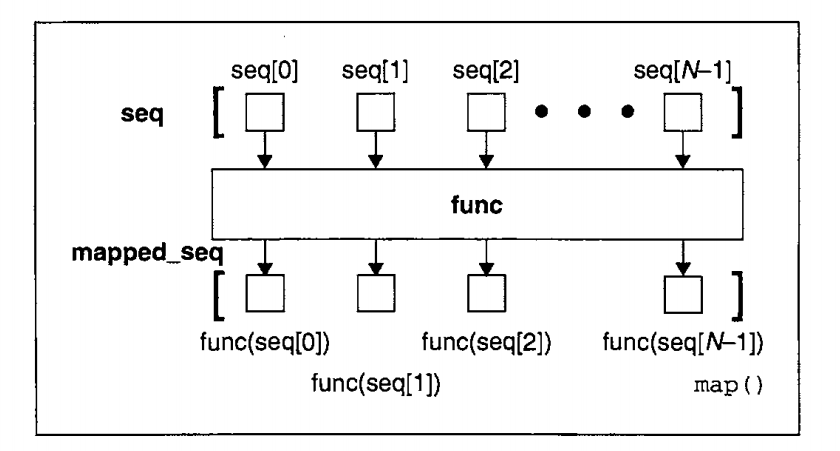
\includegraphics[height=4cm]{images/map_fuc_workprocess.jpg}
            \caption{map函数加工过程}
            \label{fig:map函数加工过程}
            \end{figure}\par
            可以看出,seq中的每个元素都经过了func函数的作用,得到了func(seq[n])组成的列表。
                \begin{lstlisting}[language=Python]
            print map( lambda x: x%3, range(6) )  #返回 [0, 1, 2, 0, 1, 2] #得到一个列表中数字%3的余数
                \end{lstlisting}\par
            并且当seq多于一个时,map可以并行地对每个seq执行,如下图(\ref{fig:map对每个seq的执行过程})所示的过程
            \begin{figure}[H]
            \centering
            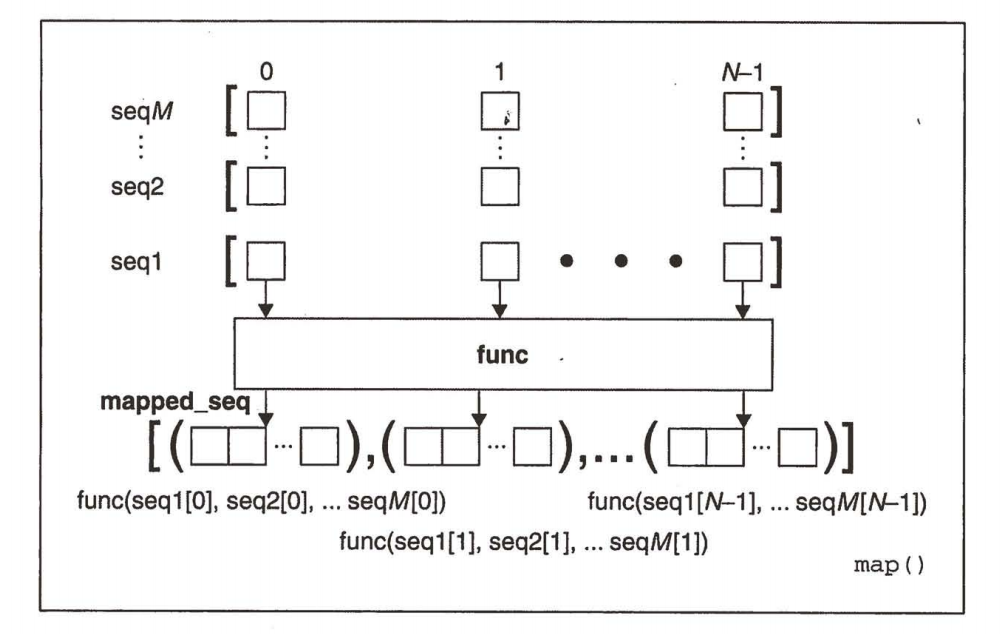
\includegraphics[height=5cm]{images/map_seq_workprocess.jpg}
            \caption{map对每个seq的执行过程}
            \label{fig:map对每个seq的执行过程}
            \end{figure}\par
            也就是说每个seq的同一位置的元素在执行过一个多元的func函数之后,得到一个返回值,这些返回值放在一个结果列表中。
            \begin{lstlisting}[language=Python]
            print map( lambda x, y: x * y, [1, 2, 3], [4, 5, 6] )  #返回[4, 10, 18]#求两个列表对应元素的积
            \end{lstlisting}
            \par
            上面的返回值是一个值的情况,实际上也可以是一个元组。下面的代码不仅实现了乘法,也实现了加法,并把积与和放在一个元组中。
                \begin{lstlisting}[language=Python]
            print map( lambda x, y: ( x * y, x + y), [1, 2, 3], [4, 5, 6] )  # 返回[(4, 5), (10, 7), (18, 9)]
                \end{lstlisting}
            \par
            下面再列举3个例子进行说明\\
            示例1:对可迭代函数'iterable'中的每一个元素应用‘function’方法,将结果作为list返回。
                \begin{lstlisting}[language=Python]
            def add100(x):
            return x+100
            hh = [11,22,33]
            map(add100,hh)
            #返回:[111, 122, 133]
                \end{lstlisting}
            示例2:如果给出了额外的可迭代参数,则对每个可迭代参数中的元素‘并行’的应用‘function’
                \begin{lstlisting}[language=Python]
            def abc(a, b, c):
            return a*10000 + b*100 + c
            list1 = [11,22,33]
            list2 = [44,55,66]
            list3 = [77,88,99]
            map(abc, list1, list2, list3)
            #返回:[114477, 225588, 336699]
                \end{lstlisting}
            示例3:如果'function'给出的是‘None’,自动假定一个‘identity’函数(相当于压缩)
                \begin{lstlisting}[language=Python]
            list1 = [11,22,33]
            list2 = [44,55,66]
            list3 = [77,88,99]
            map(None, list1, list2, list3)
            #返回:[(11, 44, 77), (22, 55, 88), (33, 66, 99)]
                \end{lstlisting}
            \par
            2、reduce的格式为:reduce( func, seq[, init] )。reduce函数即为递归,它是这样一个过程:每次迭代将上一次的迭代结果(第一次时为init的元素,如没有init则为seq的第一个元素) 与下一个元素一同执行一个二元的func函数。在reduce函数中,init是可选的,如果使用,则作为第一次迭代的第一个元素使用。下图(\ref{fig:reduce函数的工作过程})展现了reduce函数的工作过程
            \begin{figure}[H]
            \centering
            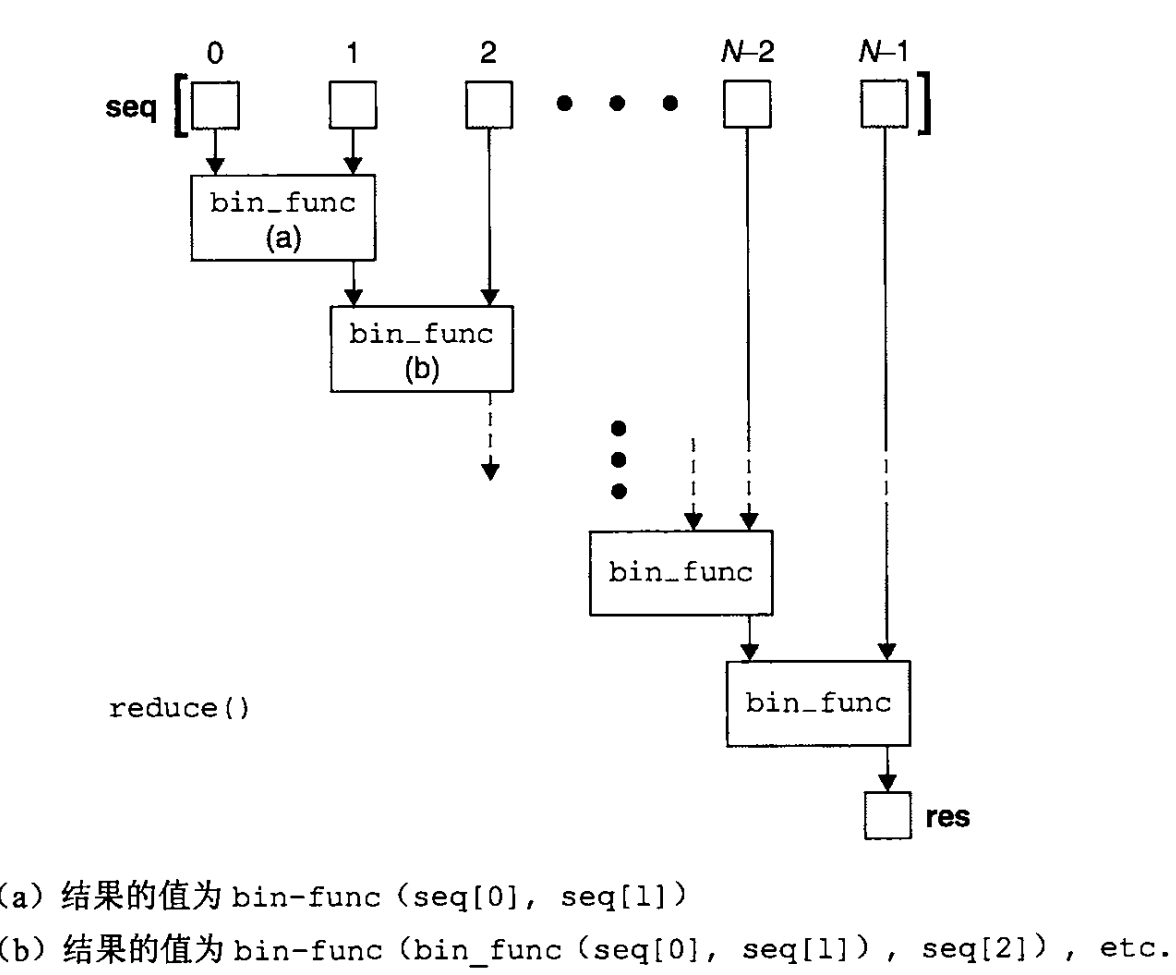
\includegraphics[height=5.5cm]{images/reduce_fuc_workprocess.jpg}
            \caption{reduce函数的工作过程}
            \label{fig:reduce函数的工作过程}
            \end{figure}
            \noindent {示例1:阶乘}
                \begin{lstlisting}[language=Python]
            print reduce((lambda x, y: x * y), range(1, 5 + 1)) #返回120是5的阶乘,(1)*2)*3)*4)*5
                \end{lstlisting}
            示例2:连加
                \begin{lstlisting}[language=Python]
            print reduce((lambda x, y: x + y), range(5)) #返回10,是(0)+1)+2)+3)+4)+5
                \end{lstlisting}
    \subsection{引入 - R和Python的基本数据结构}
            表(\ref{tab:R和Python的基本数据结构})给出了R和Python的基本数据结构,读者可将未列举的数据结构填补在表中。
            \begin{table}[H]
            \centering
            \caption{R和Python的基本数据结构}
            \label{tab:R和Python的基本数据结构}
            \newcolumntype{Y}{>{\centering\arraybackslash}X}
                \begin{tabularx}{\textwidth}{lXlX}
                \toprule
            \rowcolor{lightgray}\multicolumn{2}{l}{R}&\multicolumn{2}{l}{Python}\\\midrule
                矩阵& matrix& 字符串& str/""\\
                数组 & array&列表  &list/[]\\
                列表 & list&元组 & tuple/()\\
                数据框& data.frame&字典 & dict/$\{\}$\\
                因子 & factor&集合 & set\/frozenset\\
                时间序列 & ts&数组 & ndarray\\
                类 &class&时间序列 & series\\
                因子对象的连续性泛化 & single&数据表& DataFrame\\
                字符串& ""&数据集 &Panel\\
                \bottomrule
                \end{tabularx}
                \end{table}
    \subsection{dataset}
            可参见网址\url{http://cn.mathworks.com/help/stats/dataset.html?s_tid=gn_loc_drop}。不过,在高版本的matlab中,这个数据结构将被抛弃。

\chapter{MATLAB控制与函数}
\section{MATLAB函数}
    \subsection{函数变量及一些有用的函数}
        \par
        \begin{lstlisting}[language=Matlab]
        nargin          %在函数内,用于获取实际输入总量
        nargout         %在函数内,用于获取实际输出总量
        nargin('fun')   %返回fun函数输入参数的数量
        nargout('fun')  %返回fun函数输出参数的数量
        inputname(n)    %在函数内使用,给出第n个输入总量的实际调用变量名
        Nargchk()       %检查输入的参数个数是否符合指定的范围
        msgstr = nargchk(minargs, maxargs, numargs, 'string')  %minargs和maxargs分别为参数个数的最小值最大值,numargs为求得的输入项的项数,可直接为函数nargin如果输入变量个数超出范围,则返回错误信息;如果变量个数在范围内则返回空矩阵。
        %% 函数可变参数的输入/输出:varargin/varargout
        function y = myfunction vararg(varargin)
        temp = 0
        for i = 1:length (varargin)
            temp = temp+mean(varargin{i}(:));
        end
        y = temp/length
        end
        % 基本语法:function [y1,y2] = func(a,b, varargin)
        \end{lstlisting}
    \subsection{匿名函数(anonymous function)}
        匿名函数的格式:函数 = $@$(指定的自变量) 函数表达式,例如
        \begin{lstlisting}[language=Matlab]
        f = @(x) x^2     %表示f(x)=x^2
        f = @(x) x.^2
        fx = f(1:10)     %批量赋值,x为向量的形式,需要点乘
        f = @(x, y)x.^2 + y.^2;   %需要点乘
        \end{lstlisting}
        多层嵌套匿名函数
        \begin{lstlisting}[language=Matlab]
        f=@(a,b) @(x) a*x^2+b*x+1    %当参数a,b为未知数时,则需要用多层嵌套的匿名函数来表示。
        syms x;     %定义符号变量
        f=(x+tan(x))^(sin(x));     %定义表达式
        c=diff(f,s) %求f的3阶导数的表达式 >> f3=eval(['@(x)' vectorize(c)]);    %vectorize函数的功能是使内联函 数适合数组运算的法则。
        \end{lstlisting}
    \subsection{私有函数}
        private函数是具有访问限制的函数,对应的M文件保存在名为“private”的文件下。因为一般的matlab函数是全局可见的,而private函数只能被private文件夹所在文件夹中的函数调用。
        \begin{lstlisting}[language=Matlab]
        help private/myprivfun
        \end{lstlisting}
    \subsection{重载函数}
        一种情况下输入的几个参数为双精度浮点型,一种情况下为整型。编写两个同名函数,MATLAB会根据实际输入数据类型选择函数,但要求将函数放在不同文件夹下,文件夹名称以$@$开头,然后写数字类型,例如:$@$double、$@$int32
        matlab的函数重载是通过检查函数调用时输入输出的项数来实现。
        nargin和nargout分别返回它所在函数当前被调用时实际输入的项数。
    \subsection{内联函数 - inline}
        inline用于创建inline对象,在matlab中创建局部函数时,可用inline。在运用中有几点限制:不能调用另一个 inline函数,只能由一个matlab表达式组成,并且只能返回一个变量(显然不允许$[u,v]$这种形式)。因而,任何要求逻辑运算或乘法运算以求得最终结果的场合,都不能应用inline。
        inline调用格式如下:
        \begin{lstlisting}[language=Matlab]
        inline('expression', 'arg1','arg2', ... ,'argn');
        char(inclinefunc)       %转化为字符串
        argnames(inclinefunc)   %转化为字符串
        formula(_func)          %返回计算公式expression
        vectorize(_func)        %在函数中引入向量操作,需为点乘
        \end{lstlisting}
    \subsection{MATLAB函数句柄 - Function handle }
        包含了函数的路径、函数名、类型以及可能存在的重载方法;
        创建函数句柄的语法:fhandle = $@$function$\_$filename。例如
        \begin{lstlisting}[language=Matlab]
        fhandle = @sin    %创建了sin的句柄
        y = fhandle(pi)   %调用函数句柄,fhandle(pi)其实就是sin(pi)。
        \end{lstlisting}
        \par
        feval函数的最通常的应用是以下形式:
        feval('functionname', parameter)。
        例如:计算sin(2),可直接用命令y = sin(2);
        还可以用的方式有:
        y = feval('sin',pi/4); 或者h = @sin;y=feval(h,pi/4); 或者直接写成y = feval(@sin, pi/4)。

    \subsection{M文件一般结构}
        MATLAB中M文件有两种类型,脚本M文件和函数M文件。对于函数文件,一个M文件只能定义一个总函数,即第一句function所定义的函数,而且整个M文件在外部使用时表现出来的也只有这一个函数。如果需要多个函数嵌套,与其定义顺序无关。
        % \textcolor[rgb]{1.00,0.00,0.00}{todo:图片}
    \subsection{伪码文件—P文件(M文件保护文件)}
        当第一次执行M文件时,函数中的命令将被翻译成内部伪码格式储存在内存中,以提高后续的调用速度。伪码文件后缀为*.P,命名同*.M文件。
            \begin{lstlisting}[language=Matlab]
        pcode.filename                  %在当前目录下创建filename.p文件
        pcode(fun,'-inplace')           %在当前目录下创建filename.p文件
        clear filename                  %清除内存中的filename.p文件
        clear functions                 %清除内存中的p文件
            \end{lstlisting}
    \subsection{引入 - Python和R中的函数}
        \par
        待补充。。。

\section{控制语句}
    \subsection{MATLAB控制语句}
        \subsubsection{分支判断语句(if-else-end结构)}
            \par
            (1)如果是…那么…
             \begin{lstlisting}[language=Matlab]
            if expression         %逻辑表达式
               commands           %命令/程序
            end
            \end{lstlisting}
            \par
            (2)如果是…那么…,否则…
            \begin{lstlisting}[language=Matlab]
            if expression
               commands1         %如果条件为真则执行commands1
            else
               commands2         %如果条件为假则执行commands2
            end
            \end{lstlisting}
            \par
            (3)如果可选择的执行命令组有多组,则调用下面结构
            \begin{lstlisting}[language=Matlab]
            if expression1
               commands1         %如果条件expression1为真则执行commands1
            elseif expression2
               commands2         %如果条件expression2为真则执行commands2
            ...
            else
               commandsn         %如果前面的所有条件都不满足就执行最后一条
            end
                \end{lstlisting}
        \subsubsection{分支选择语句(switch - case)}
            计算expression,如果结果为case*后的value*时,则执行对应的commands
                \begin{lstlisting}[language=Matlab]
            switch expression
                 case test1
                      commands1
                 case test2
                      commands2
                 ...
            otherwise
                      commandsn %如果所有的条件都不满足就执行这条命令
            end
                \end{lstlisting}
        \subsubsection{循环控制语句}
            第一种循环-for循环
                \begin{lstlisting}[language=Matlab]
            for ...
            end
                \end{lstlisting}
            \par
            第二种循环-while循环
                \begin{lstlisting}[language=Matlab]
            while expression    %直到逻辑否时,退出循环
            end
                \end{lstlisting}
            % \textcolor[rgb]{1.00,0.00,0.00}{注:循环之前需分配变量}
        \subsubsection{尝试控制(try - catch)}
                \begin{lstlisting}[language=Matlab]
            try
                command1  %尝试执行command1,若正确,则catch下的命令组将不会被执行
            catch
                command2  %如果command1命令组执行出错了,该命令组将被执行
            end
            \end{lstlisting}
            如果在catch下的command2的命令组的执行过程也出错了,那么Matlab将停止运行。
            \begin{lstlisting}[language = Matlab]
            try
                command1  %尝试执行command1,若出错end后的信息仍然可以执行
            end
            try
                command1  %尝试执行command1,若正确,则catch下的命令组将不会被执行
            catch error %如果command1命令组执行出错了,记录错误到error,并执行command2
                command2
            end
                \end{lstlisting}
        \subsubsection{其它命令}
                \begin{lstlisting}[language=Matlab]
            pause       %暂停
            pause       %暂停执行文件,等待用户按任意键继续
            pause(n)    %在继续执行文件之前,暂停n秒
            pause on/off%允许/不允许后面程序暂停
            lasterr     %可以显示matlab系统判断的最新出错原因。
            lastwarn    %可以显示matlab系统给出的最新警告程序并继续运行。
            break       %跳出循环体,执行end后面的语句。如果是多层循环(for for for),break只能跳出其所在的\\循环,如果break在最外层循环,则跳出所有循环。用在分支中 (switch... case)即不执行此分支\\块的下面的语句。但执行end后的语句。
            return      %终止(就是直接退出程序或函数返回了)
            error using %调用某函数出错(函数本身没错),如参数不对,格式错等
            error in    %某函数内部出错
            error('message');   %显示错误信息并终止程序
            warning('message'); %显示错误信息,继续程序
                \end{lstlisting}
            留白以补充:\par
            input命令将Matlab的控制权暂时交给用户,等待用户通过键盘输入数值、字符串或表达式等并经回车键将输入内容传递到工作空间后,收回控制权。\par
            keyboard命令将控制权交给键盘,用户可以由键盘输入各种合法的matlab命令,只有当用户输入完成,并键入return命令后,才收回控制权。\par
            input命令和keyboard命令的不同之处在于:keyboard命令允许输入任意多个Matlab命令,而input命令只允许用户输入赋值给变量的数组、字符串或元胞数组等。\par
    \subsection{Python控制语句}
        \subsubsection{1、分支判断语句(if:else结构)}
            (1)如果是…那么…(注意Python的控制语句要有空格,以及$:$提示符)
                \begin{lstlisting}[language=Python]
            if expression:
                command
                \end{lstlisting}
            \par
            (2)如果是…那么…,否则…
                \begin{lstlisting}[language=Python]
            if expression:
                command1
            else:
                command2
                \end{lstlisting}
            \par
            (3)如果可选择的执行命令组有多(n)组,则调用下面结构
                \begin{lstlisting}[language=Python]
            if expression:
                command1
            elif  expression:
                command2
            ...
            else:
            command
                \end{lstlisting}
        \subsubsection{2、循环控制语句}
            第一种循环 - while循环
            \begin{lstlisting}[language=Python]
            while expression:  #直到逻辑否时,退出循环。
                command
            while expression:
                command
            else:
                command
            \end{lstlisting}
            注:与本文后面介绍的 for 循环一样,while支持三种附加语句:continue、 break和 pass。
            Python中没有switch case循环。在循环完成后执行else,当有break时,会跳过else。
            \par
            第二种循环 - for循环
            \begin{lstlisting}[language=Python]
            for itervar in interable:
                command
            for itervar in interable:
                command
            else:
                command
            \end{lstlisting}
            注:interable是range(start, end, step ),可迭代类。
            Python2.3新增enumerate,通过项和索引进行迭代,例如:
                \begin{lstlisting}[language=Python]
            for i, eachlee in enumerate(list):
                 print “%d %s lee” %(i+1, eachlee)
                \end{lstlisting}
        \subsubsection{3.异常捕获try}
            \par
            (1)try:except:else:
            \begin{lstlisting}[language=Python]
            try:
                command1
            except:
                command2
            ......
            else:
                command3
            \end{lstlisting}
            注:当开始一个try语句后,python就在当前程序的上下文中作标记,这样当异常出现时就可以回到这里,try子句先执行,接下来会发生什么依赖于执行时是否出现异常。如果command1出现异常,执行command2,如果不存在异常执行command3。
            \par
            1、如果当try后的语句执行时发生异常,python就跳回到try并执行第一个匹配该异常的except子句,异常处理完毕,控制流就通过整个try语句(除非在处理异常时又引发新的异常)。\par
            2、如果在try后的语句里发生了异常,却没有匹配的except子句,异常将被递交到上层的try,或者到程序的最上层(这样将结束程序,并打印缺省的出错信息)。\par
            3、如果在try子句执行时没有发生异常,python将执行else语句后的语句(如果有else的话),然后控制流通过整个try语句。
            \par
            (2)try:finally:
            \begin{lstlisting}[language=Python]
            try:
                command1
            finally:
                command2
            \end{lstlisting}
            注:python总会执行finally子句,无论try子句执行时是否发异常。\ding{172}如果没有发生异常,python运行try子句,然后是finally子句,然后继续。\ding{173}如果在try子句发生了异常,python就会回来执行finally子句,然后把异常递交给上层try,控制流不会通过整个try语句。
            \par
            (3)try:else:
            \begin{lstlisting}[language=Python]
            try:
                command1
            except Exception[, reason1]:    #例valueError
                command2
            except Exception[, reason2]:    #例TypeError
                command3
            else:
                commandn
            \end{lstlisting}
            注:1、如果command1没有异常,忽略所有的except继续执行;如果command2出现异常,在所有except子句中寻找匹配异常,并执行其后的command。\par
            2、expect可选项如下:
            \begin{itemize}
              \item except: 捕获所有异常;
              \item except name: 只捕获特定的异常;
              \item except name, value: 捕获异常和它的附加数据(将异常的信息保存到value);
              \item except (valueError, TypeError): 捕获任何列出的异常;
            \end{itemize}
        \subsubsection{4、其他命令}
            \begin{lstlisting}[language = Python]
            break    # 跳出逐层循环体。
            continue # continue语句会让当前的迭代结束,忽略其后语句(command),直接开始下一轮的循环。如果是条件循环(while),验证条件表达式expression;如果是迭代循环(for),验证是否还有元素可以迭代,如果验证有,则进行迭代。
            pass     # 代码中的占位符: pass语句在Python代码中充当占位符使用。在不要执行任何东西时可以暂时使用pass语句来填充。
            \end{lstlisting}
            留白以补充:\par
            列表推导式(list comprehension)是利用其它列表创建新列表的一种方法;\par
            使用exec语句可以执行存储在字符串中的Python代码;\par
            通过使用eval语句可以计算以字符串形式书写的Python表达式。
    \subsection{R控制语句}
        \subsubsection{1、分支判断语句}
            \par
            (1)如果是…那么…
                \begin{lstlisting}[language=R]
            if (expression){
               commands
            }
            \end{lstlisting}
            \par
            (2)如果是…那么…,否则…
            \begin{lstlisting}[language = R]
            if (expression) command1 else command2
            if (expression) {command1} else {command2}
            if (expression) {
            commdan1
            } else {
            commdan2
            }
            \end{lstlisting}
            \par
            (3)如果可选择的执行命令组有多组,则调用下面结构
            \begin{lstlisting}[language = R]
            if (expression1) {
               commands1
            } elseif (expression2) {
               commands2
            ...
            }else{
               commandsn
            }
            \end{lstlisting}
            注:1.将 \{ 放在当前行,而非单独一行\footnote{Google内部R程序规范}。
            \par
            2. ifelse(expression, a, b) \#当expression[i]为真时,返回$a[i]$,否则返回$b[i]$。
        \subsubsection{2、分支选择语句}
        \subsubsection{3、循环语句}
            \par
            (1)第一种循环 - while循环
                \begin{lstlisting}[language=R]
              while (expression) {
                commands
                }
                \end{lstlisting}
            \par
            (2)第二种循环 - for循环
                \begin{lstlisting}[language=R]
                for (I in expression) {
                commands
                }
                \end{lstlisting}
            \par
            (3)第三种循环 - repeat循环
              \begin{lstlisting}[language=R]
              repeat expression
              #示例:i <-5
              repeat {if (I > 25) break else {print(i); i <- i+5;}}
              \end{lstlisting}
            \par
            (4)第四种循环 - foreach循环。foreach来自于foreach包,能够遍历向量、矩阵、数据框或者迭代器。其命令格式为:
                \begin{lstlisting}[language=R]
                foreach(..., .combine, .init,
                              .finall = NULL,
                              .inorder = TURE,
                              .multicombine = FALSE,
                              .maxcombine = if (.multicombine) 100 else 2,
                              .errorhandling = c(‘stop’, ‘remove’, ‘pass’),
                              .packages = NULL,
                              .export = NULL,
                              .noexport= NULL,
                              .berbose = FALSE)
                # 示例:
                foreach(a = 1:3, b = rep(10, 3)) %do%{
                a + b
                } #可用%dopar%实现并行操作
                \end{lstlisting}
        \subsubsection{4、异常捕获语句}
                \begin{lstlisting}[language=R]
                trycatch(
                {expression},
                warning = function(w) {warning-handle-code},
                error = function(e) {error-handle-code},
                finally = {clean up-code}
                )
                \end{lstlisting}
            注:如果有warning发生,执行warning-handle-code,如果有error发生,执行error-handle-code,如果有finally,无论是否发生,都执行clean up-code。
            try (expression, silent) \#expression为要尝试的内容,$silent = T/F$,表示是否将错误信息返回控制台。
        \subsubsection{5、其他命令}
                \begin{lstlisting}[language=R]
            iter  #存在于iterators包中,用nextElem查看迭代项。
            iter(obj, chechFunc = function() TRUE, recycle = FALSE, …)
                \end{lstlisting}
            其中:obj是迭代目标,checkFunc指定一个过滤迭代器返回值的函数,recycle指定当对象元素迭代结束后是否对迭代进行重置。
            示例:
                \begin{lstlisting}[language=R]
            myfirst <- iter(1:5)
            nextElem(myfirst)
            break
            next
            stop
            warning
                \end{lstlisting}
            留白以补充:\\
            ls、ls.str、edit


% \bibliography{part-matlab-chap-drawing}%bib文件名称
% \end{document}

